\chapter{An Asymptotic Test for Conditional Independence using Analytic Kernel Embeddings}
\label{paper:kerneltest}
We propose a new conditional dependence measure and a statistical test for conditional independence. The measure is based on the difference between analytic kernel embeddings of two well-suited distributions evaluated at a finite set of locations. We obtain its asymptotic distribution under the null hypothesis of conditional independence and design a consistent statistical test from it. We conduct a series of experiments showing that our new test outperforms state-of-the-art methods both in terms of type-I and type-II errors even in the high dimensional setting.
 %while being fast to evaluate. 
% The proposed tests are easy to implement and we lead experiments to validate our claims on both synthetic and real 
\section{Introduction}
We consider the problem of testing whether two variables $X$ and $Y$ are independent given a set of confounding variables $Z$, which can be formulated as a hypothesis testing problem of the form:
\begin{align*}
    H_0:~ X\perp Y | Z\qquad\text{vs.}\qquad H_1:X\not\perp Y | Z.
\end{align*}
Testing for conditional independence (CI) is central in a wide variety of statistical learning problems. For example, it is at the core of graphical modeling~\citep{lauritzen1996graphical,koller2009probabilistic}, causal discovery~\citep{pearl2009causal,glymour2019review}, variable selection \citep{candes2018panning}, dimensionality reduction~\citep{li2018sufficient}, and biomedical studies~\citep{richardson1993bayesian,dobra2004sparse,markowetz2007inferring}. 
 
Testing for $H_0$ in such applications is known to be a highly challenging task~\citep{gcm2020,neykov2021minimax}. A large line of work has focused on the design of measures for conditional dependence based for example on kernel methods~\cite{fukumizu2008kernel,Sheng2019OnDA,NEURIPS2020_f340f1b1,huang2020kernel} and rank statistics~\cite{azadkia2021simple,shi2021azadkia}. Testing for conditional independence is even a more difficult as it requires both designing a test statistic which measures the conditional dependencies and controlling its quantiles. Indeed, existing tests may fail to control the type-I error, especially when the confounding set of variables is high-dimensional with a complex dependency structure~\cite{bergsma2004testing}. Furthermore, even if the test is valid, the availability of limited data makes the problem of discriminating between the null and alternative hypotheses extremely difficult, resulting in a test of low power. These challenges has motivated the development of a series of practical methods attempting to reliably test for conditional independence. These include tests based on kernels ~\citep{zhang2012kernel,doran2014permutation,strobl2019approximate,Zhang2017FeaturetoFeatureRF}, ranks~\cite{runge2018conditional,mittag2018nonparametric}, models~\citep{sen2017modelpowered,sen2018mimic,chalupka2018fast,gcm2020}, permutations and  samplings~\citep{berrett2020conditional,candes2018panning,BellotS19, shi2021double,javanmard2021pearson},
and optimal transport~\cite{warren2021wasserstein}.



% In addition, estimating conditional independence  may become computationally expensive as the dimension of the problem increases. For example, the Kernel Conditional Independence Test (KCIT)~\citep{zhang2012kernel} requires a cubic number of operations with respect to the sample size. Moreover, in this setting, any bootstrap or permutation procedure becomes expensive as one needs to compute multiple times the statistic of interest. Such strategies are often used to estimate the p-value as the (asymptotic) null distribution, which may be parameter dependent~\citep{sen2017modelpowered,shi2021double}. In that context, \citet{strobl2019approximate} propose to reduce the computational complexity of KCIT by considering a Random Fourier features approximations of the kernels involved in the statistic, resulting in a test that scales linearly with respect to the sample size. 

% We explore in this work similar ideas in order to approximate the proposed statistic and obtain a linear time test for conditional independence.
% Kernel methods offer a general and successful framework for capturing (conditional) dependence of variables. However estimating conditional independence  may become computationally expensive as the dimensions of the problem increase. For example, the Kernel Conditional Independence Test (KCIT)~\citep{zhang2012kernel} scales at least quadratically with sample size. In \cite{strobl1702approximate}, the authors propose to reduce the time complexity of KCIT by considering a Random Fourier features approximations of the kernels involved in the statistic and obtain a test which scales linearly with respect to the sample size. We explore in this work similar ideas in order to approximate the  proposed statistic and obtain a linear time test for conditional independence.


In this paper, we propose a new kernel-based test for conditional independence with asymptotic theoretical guarantees.
% Given samples $(X,Y,Z)$ from the joint distribution $P_{XYZ}$, we aim at testing the independence of $X$ and $Y$ conditionally to $Z$. 
Taking inspiration from~\cite{chwialkowski2015fast,jitkrittum2017adaptive,NEURIPS2019_0e2db0cb}, we use the $\ell^p$ distance between two well-chosen analytic kernel mean embeddings evaluated at a finite set of locations. We show that this measure encodes the conditional dependence relation of the random
variables under study. 
% From this metric, we derive a new conditional dependence measure which can scale linearly with respect to the number of samples. 
Under common assumptions on the richness of the RKHS, we derive the asymptotic null distribution of our measure, and design a simple nonparametric test that is distribution-free under the null hypothesis. Furthermore, we show that our test is consistent. Lastly, we validate our theoretical claims and study the performance of the proposed approach using simulated conditionally (in)dependent data and show that our testing procedure outperforms state-of-the-art methods.


\subsection{Related Work}
% \cite{fukumizu2008kernel} was the first paper to introduce a kernel-based measure of conditional dependence. The authors presented the conditional cross-covariance operator as a way to characterize the conditional relation between $X$ and $Y$ given $Z$. They also showed how to estimate this operator, however, without offering a testing procedure that is based on it. Moreover, the asymptotic distribution of the statistic from \cite{fukumizu2008kernel} is unknown.


\citet{zhang2012kernel} propose a kernel based-test (KCIT), by leveraging the characterization of conditional independence derived in \citep{daudin1980partial} to form a test statistic. The authors of this work obtain the asymptotic null distribution of the proposed statistic and derived a practical procedure from it to test for $H_0$. However, one main practical issue of the proposed test is that the asymptotic null distribution of their statistic cannot be computed directly as it involved unknown quantities. To address this problem, the authors propose to approximate it either with Monte Carlo simulations or by fitting a Gamma distribution. In our work, we propose a new kernel-based statistic to test for conditional independence and show that its asymptotic null distribution is simply the standard normal distribution. In addition \citet{zhang2012kernel} extended the Gaussian process (GP) regression framework to the multi-output case, which allowed them to find the hyperparameters involved in the test statistic, maximizing the marginal likelihood. We also deploy a similar optimization procedure to that of \citet{zhang2012kernel}, however, in our case the output of the GP regression is univariate and therefore more computationally efficient.

% \citet{zhang2012kernel} proposed a kernel based-test (KCIT), by leveraging the characterization of conditional independence derived in \citep{daudin1980partial} to form a test statistic. The authors of this work analyzed the asymptotic distribution of the proposed statistic, offering a practical procedure to test for $H_0$. In addition, \citet{zhang2012kernel} extended the Gaussian process (GP) regression framework to the multi-output case, which allowed them to find the hyperparameters involved in the test statistic, maximizing the marginal likelihood. However, this test is computationally expensive since both the estimation of the p-value as well as the computation of the statistic require at least a cubic number of operations. In our work, we propose a new kernel-based statistic that is computationally efficient, which scales linearly with the number of samples. We also deploy a similar optimization procedure to that of \citet{zhang2012kernel}, however, in our case the output of the GP regression is univariate. In addition, the p-values of the proposed test are easy to obtain: we show that the asymptotic null distribution of our statistic follows the standard normal distribution.



Other CI tests proposed in the literature suggest testing relaxed forms of conditional independence. For instance,~\citet{gcm2020} propose the generalised covariance measure (GCM) which only characterises weak conditional dependence~\cite{daudin1980partial} and \citet{Zhang2017FeaturetoFeatureRF} propose a kernel-based test which focuses only on individual effects of the conditioning variable $Z$ on $X$ and $Y$. Some other tests are based on the knowledge of the conditional distributions in order to measure conditional dependencies. For example \citet{candes2018panning} assume that one has access to the exact conditional distributions,~\citet{BellotS19,shi2021double} approximate them using generative models and \citet{sen2017modelpowered} consider model-based methods to generate samples from the conditional distributions. In our work, we design a test statistic which characterizes the exact conditional independence of random variables and obtain its asymptotic null distribution without assuming any knowledge on the conditional distributions. Under some mild assumptions on the RKHSs considered, we also derive an approximate test statistic which admits the same asymptotic distribution and obtain a simple testing procedure from it.




% Although the application might seem immediate from~\citet{NEURIPS2019_0e2db0cb}, one need either to sample or estimate an expectation conditionally to $X$. While the option of sampling is impossible in practice, estimation of the conditional expectation can be done using Regularized Least Squares (RLS) as it was done by~\cite{zhang2012kernel}. Using this estimation in the test statistic asks convergence questions we tackle in this paper by a rigorous analysis using convergence rates of RLS from~\citep{fischer2017sobolev}. To ensure this convergence, assumptions on the spectrum and a source condition are required.  

% \textbf{Outline } We begin by providing the required background on kernels and conditional independence testing. Then, we turn to introduce a new statistic to measure conditional dependency. To avoid costful bootstrap or permutation procedures {\color{red}[what is the goal? to estimate what?]}, We also propose a normalized version of this statistic. Under some assumptions, we derive the asymptotic law of our statistics both for the null and alternative hypothesis. We also propose a random feature relaxation to accelerate the computation of the statistic. Finally, we use simulated data to validate our theoretical claims as well as to study the performance of our approach.





% \section{Related Work}
 


% In the latter work~\citep{strobl1702approximate}, the authors extended the work from~\cite{zhang2012kernel} to random features to get a fast computation of the statistic. In this paper, the authors get the law for an oracle estimator of the conditional expectation. We also propose a random Fourier estimation of our statistic, but leave as further the proof of its consistency.

% \cite{zhang2012kernel} introduced a
% kernel-based test for conditional independence testing (KCIT), offering a
% test statistic that can potentially asses all the moments of the joint distribution of $X$, $Y$, and $Z$. The test is accompanied with a type I error control guarantee that holds asymptotically in the number of samples. One limitation of this test is that it may become computationally infeasible as the dimensions of the problem increase: it scales at least quadratically with sample size. In response, \cite{strobl1702approximate} reduce the time complexity of KCIT by considering a Random Fourier features approximations of the kernels involved in the statistic and obtain a test which scales linearly with respect to the sample size. In this paper, we explore similar ideas in order to approximate the our proposed statistic and obtain a linear time test for conditional independence.
% .



% \begin{itemize}
%     \item Expliquer que pour \cite{zhang2012kernel}: l'obtention de la loi n'est pas clair mais qu'avec des hypotheses supplementaires sur la convergence en proba le resultat tient.
%     \item Expliquer pour \cite{strobl1702approximate} l'obtention de la loi asymptotique n'est obtenu que pour un estimateur oracle de la l'esperance conditionnel mais qu'aucun resultat n'est donne pour la loi asymptotique lorsque l'on emploie des RF.
% \end{itemize}

% \textbf{Covariance Operator.} Let $(\mathcal{D}_1,\mathcal{A}_1)$ and $(\mathcal{D}_2,\mathcal{A}_2)$ two measurable spaces, $(H_1,k_1)$ and $(H_2,k_2)$ two measurable reproducing kernel Hilbert spaces (RKHS) on respectively $\mathcal{D}_1$ and $\mathcal{D}_2$ respectively and let $\nu\in\mathcal{M}_{1}^{+}(\mathcal{D}_1\times\mathcal{D}_2)$. If  $\mathbb{E}_{(x,y)\sim\nu}[k_{1}(x,x)]$, and  $\mathbb{E}_{(x,y)\sim\nu}[k_{2}(y,y)]$ are finite, then there exists a unique operator $\Sigma_{\nu}^{k_1,k_2}$ from $H_1$ to $H_2$ such that for all $(f,g)\in H_1\times H_2$,
% \begin{align*}
%     \langle g,\Sigma_{\nu}^{k_1,k_2}f\rangle_{H_2} = \mathbb{E}_{(x,y)\sim\nu}(f(x)g(y))\; .
% \end{align*}

% A close link exists between the mean embedding and the covariance operator. Indeed by defining for all $x,x'\in\mathcal{D}_1$ and $y,y'\in\mathcal{D}_2$ the measurable kernel $k_1\cdot k_2 ((x,y),(x',y'))=k_1(x,x')k_2(y,y')$ on $\mathcal{D}_1\times\mathcal{D}_2$ with corresponding RKHS $H_1\otimes H_2$, the tensor-product space of $H_1$ and $H_2$, one obtains that for all $(t_1,t_2)\in\mathcal{D}_1\times \mathcal{D}_2$
% \begin{align*}
%     \mu_{\nu,k_1\cdot k_2}(t_1,t_2)=\langle k_2(t_2,\cdot),\Sigma_{\mu}^{k_1,k_2}k_1(t_1,\cdot)\rangle_{H_2}\; .
% \end{align*}


\section{Background and Notations}
We first recall some notions on kernels and mean embeddings which will be useful in the derivation of our conditional independence test.
% \paragraph{$\ell^p$-distance between mean embeddings.}  Non-parametric two sample using kernels has been widely studied in literature. At first, GRETTON proposed to use the maximum mean discrepancy (MMD) to build a consistent statistical test. ADD a bit more of text 
% More recently, REF proposed to study closely related two sample tests.
% ADD REF Introduce Lp two sample test and notations
% \paragraph{Independence testing}
% Explain here the link with covariance operator gretton Scholkoff ect formally also + Witt test with L2 metric: S and g considers the MMD distance between mean embeddings while Witt consider the L2 distance. 
Let $(\mathcal{D},\mathcal{A})$ be a Borel measurable space and denote $\mathcal{M}_{1}^{+}(\mathcal{D})$ the space of Borel probability measures on $\mathcal{D}$. Let also $(H,k)$ be a measurable RKHS  on $\mathcal{D}$, i.e. a functional Hilbert space satisfying the reproducing property: for all $f\in H$, $x\in\mathcal{D}$, $f(x)=\langle f,k_x\rangle_H$. Let $\nu\in\mathcal{M}_{1}^{+}(\mathcal{D})$. If $\mathbb{E}_{x\sim\nu}[\sqrt{k(x,x)}]$ is finite, we define for all $t\in\mathcal{D}$ the \emph{mean embedding} as $\mu_{\nu,k}(t):=\int_{x\in\mathcal{D}}k(x,t)d\nu(x)$.
Note that $\mu_{\nu,k}$ is the unique element in $H$ satisfying for all $f\in H$,  $\mathbb{E}_{x\sim\nu}(f(x))=\langle \mu_{\nu,k},f\rangle_{H}$. If  $\nu\mapsto\mu_{\nu,k}$ is injective, then  the kernel $k$ is said to be \emph{characteristic}. This property is essential for the separation property to be verified when defining a kernel metric between distributions, such as the MMD~\citep{gretton2012kernel}, or the $\ell^p$ distance~\citep{NEURIPS2019_0e2db0cb}. % For instance the t
% \textbf{Characteristic and analytic kernels.} A kernel $k$ is said to be characteristic if  $\nu\mapsto\mu_{\nu,k}$ is injective. This property is essential for separation property to be verified when defining a kernel metric between distributions as MMDs~\citep{gretton2012kernel}, or $\ell^p$ distances~\citep{chwialkowski2015fast,jitkrittum2017adaptive,NEURIPS2019_0e2db0cb}. An analytic kernel on $\mathbb{R}^d$ is a positive definite kernel such that for all $x\in\mathbb{R}^d$, $k(x,\cdot)$ is an analytic function, i.e., a function defined locally by a convergent power series. Remark that the tensor-product of two analytic kernel is still analytic.% For instance the t
% %Speak about the gaussian case: \textbf{Example of Tensor-product Analytic Kernels.} Explain the gaussian case. Here note that the evaluation of the kernels requires only $\mathcal{O}(d_1+d_2)$ algebraic operations.

\textbf{$\ell^p$-distance between mean embeddings.} Let $k$ be a definite positive, characteristic, continuous, and bounded kernel on $\mathbb{R}^d$ and $p\geq 1$ an integer. \citet{NEURIPS2019_0e2db0cb} showed that given an absolutely continuous Borel probability measure $\Gamma$ on $\mathbb{R}^d$, the following function defined for any  $(P,Q)\in\mathcal{M}_1^{+}(\mathbb{R}^d)\times\mathcal{M}_1^{+}(\mathbb{R}^d)$ as 
\begin{align}
\label{eq-dlp}
    d_{p}(P,Q):=\left[\int_{\mathbb{R}^d}|\mu_{P,k}(\mathbf{t})-\mu_{Q,k}(\mathbf{t})|^p d\Gamma(\mathbf{t})\right]^{\frac{1}{p}}
\end{align}
is a metric on $\mathcal{M}_1^{+}(\mathbb{R}^d)$.
% Therefore we have a simple characterization of independence.
% Indeed $d_{L^{p},k}^p(P_{XY},P_X\otimes P_Y)=0$ if and only if $X\perp Y$.
%  Remark that the tensor-product of two analytic kernel is still analytic. 
When the kernel $k$ is analytic\footnote{An \emph{analytic kernel} on $\mathbb{R}^d$ is a positive definite kernel such that for all $x\in\mathbb{R}^d$, $k(x,\cdot)$ is an analytic function, i.e., a function defined locally by a convergent power series.}, \citet{NEURIPS2019_0e2db0cb} also showed that for any $J\geq 1$, 
\begin{align}
\label{eq-dlp_J}
    d_{p,J}(P,Q):=\left[\frac{1}{J}\sum_{j=1}^J |\mu_{P,k}(\mathbf{t}_j)-\mu_{Q,k}(\mathbf{t}_j)|^p\right]^{\frac{1}{p}},
\end{align}
where $(\mathbf{t}_j)_{j=1}^J$ are sampled independently from the $\Gamma$ distribution, is a random metric\footnote{A random metric is a random process which satisfies all the conditions for a metric almost-surely.} on $\mathcal{M}_1^{+}(\mathbb{R}^d)$.
% \textbf{Smooth Characteristic Functions.}  Define what is A smooth characteristic function,
% \paragraph{Regularized Least-Square Estimator.} Define the RLS estimator in general and give sufficient condition for the RLS estimator to converge in L2.



In what follows, we consider distributions on Euclidean spaces. More precisely, let $d_x,d_y,d_z\geq 1$, $\mathcal{X}:=\mathbb{R}^{d_x}$, $\mathcal{Y}:=\mathbb{R}^{d_y}$, and $\mathcal{Z}:=\mathbb{R}^{d_z}$. Let $(X,Z,Y)$ be a random vector on $\mathcal{X}\times\mathcal{Z}\times\mathcal{Y}$ with law $P_{XZY}$. We denote by $P_{XY}$, $P_X$, and $P_Y$ the law of $(X,Y)$, $X$, and $Y$, respectively. We also denote by $\mathcal{\ddot{X}}:=\mathcal{X}\times\mathcal{Z}$, $\ddot{X}:=(X,Z)$, and $P_{\ddot{X}}$ its law. Let $P_X\otimes P_Y$ be the product of the two measures $P_X$ and $P_Y$. Given $(H_{\mathcal{\ddot{X}}},k_\mathcal{\ddot{X}})$ and $(H_{\mathcal{Y}},k_{\mathcal{Y}})$, two measurable reproducing kernel Hilbert spaces (RKHS) on $\mathcal{\ddot{X}}$ and $\mathcal{Y}$, respectively, we define the tensor-product RKHS $H=H_{\mathcal{\ddot{X}}}\otimes H_\mathcal{Y}$ associated with its \emph{tensor-product kernel} $k=k_{\mathcal{\ddot{X}}}\otimes k_{\mathcal{Y}}$, defined for all $\ddot{x},\ddot{x}'\in\mathcal{\ddot{X}}$ and $y,y'\in\mathcal{Y}$, as $k((\ddot{x},y),(\ddot{x}',y'))= k_{\mathcal{\ddot{X}}}(\ddot{x},\ddot{x}')\times k_{\mathcal{Y}}(y,y').$














% \paragraph{Random features.} Let $\mathcal{H}$ be a RKHS with kernel $k$ on ground space $\mathcal{X}$. Let assume that $k$ admits the following decomposition: 
% \begin{align*}
%     k(x,y) = \mathbb{E}_{w\sim P}\left(\phi(w,x)^T\phi(w,y)\right)
% \end{align*}
% where $P$ is a distribution on some space $\mathcal{W}$ and $\phi:\mathcal{W}\times\mathcal{X}\mapsto \mathbb{R}^p$. Without loss of generality we will assume in the following that $p=1$.
% Then using MC estimation one estimation:
% ADD PROPERTY OF UNIFORM CONVERGENCE TO THE KERNEL


% We now assume that $k_\mathcal{X}$, $k_\mathcal{Y}$ and $k_\mathcal{Z}$ admits a random features decomposition. Let denote $\widehat{\phi_\mathcal{X}} = \left(\phi^1_\mathcal{X},\dots,\phi^{r_\mathcal{X}}_\mathcal{X}\right)$, the features such that $k_\mathcal{X}(x,y)\simeq \widehat{\phi_\mathcal{X}} (x)^T\widehat{\phi_\mathcal{X}} (y)$. In this case: 
% \begin{align*}
% \langle\Sigma_{YX},\phi_X(t_1)\otimes \phi_Y(t_2)\rangle_{\mathcal{H}_X\otimes\mathcal{H}_Y} \simeq \widehat{\phi_\mathcal{X}}(t_1)^TC_{YX} \widehat{\phi_\mathcal{Y}}(t_2)
% \end{align*}
% where $(C_{YX})_{ij} = \cov_{(X,Y)\sim p_{XY}} (\phi^i_\mathcal{X}(X),\phi^j_\mathcal{Y}(Y))$. Then one can estimate $C_{YX}$ using empirical estimates of covariances. We denote $\widehat{C_{YX}}$ this estimate.

% One can then also estimate the conditional covariance operator in this case. 
% More over one can notice that:
% \begin{align*}
% \left(C_{XZ}C_{ZZ}^{-1/2}\right)_{i,j}= \frac{\cov_{(X,Z)\sim p_{XZ}}(\phi^i_\mathcal{X}(X),\phi^j_\mathcal{Z}(Y))}{\sqrt{\var_{Z\sim p_Z}(\phi^j_\mathcal{Z}(Z))}}    
% \end{align*}



% \subsection{Kernel measures of independence}

% Then a natural extension of $XXX$ and $XXX$ to measure condition independence is:
% \begin{align*}
%     D_1&(p_{XY},p_X\otimes p_Y)\\ &=\mathbb{E}_{(t_1,t_2)\sim\Gamma}\left(\lvert\langle \Sigma_{YX},\phi_X(t_1)\otimes \phi_Y(t_2)\rangle_{\mathcal{H}_X\otimes\mathcal{H}_Y}\rvert\right)
% \end{align*}



% \section{Kernel measures of conditional independence}
% % DEFINE kernel and RKHS
% % $\Sigma_{XY|Z}=\Sigma_{XY}-\Sigma_{XZ}\Sigma_{ZZ}^{-1}\Sigma_{ZY}$
% % Without loss of generality, up to an isometry, this operator can be seen as elements of $\mathcal{H}_X\otimes\mathcal{H}_Y$ Then, in $\mathcal{H}_X\otimes\mathcal{H}_Y$, the mean embedding of $p_{XY}-p_{X}\otimes p_Y$ is $\Sigma_{XY}$ and the one of $\mathbb{E}_Z\left(p_{X|Z}\otimes p_{Y|Z}\right) -p_{X}\otimes p_Y$ (Check a centralized version) is $\Sigma_{XZ}\Sigma_{ZZ}^{-1}\Sigma_{ZY}$. 

% Then a natural extension of $XXX$ and $XXX$ to measure condition independence is:
% \begin{align*}
%     D_1&(p_{XY},\mathbb{E}_Z\left(p_{X|Z}\otimes p_{Y|Z}\right) )\\ &=\mathbb{E}_{(t_1,t_2)\sim\Gamma}\left(\lvert\langle \Sigma_{YX|Z},\phi_X(t_1)\otimes \phi_Y(t_2)\rangle_{\mathcal{H}_X\otimes\mathcal{H}_Y}\rvert\right)
% \end{align*}



%\section{A First Independence Test}
Here we extend the framework proposed in~\cite{jitkrittum2017adaptive} to the $\ell^p$ geometry for any $p\geq 1$ and design of a new nonparametric statistical tests of dependence: that is, tests of whether a joint distribution $P_{XY}$ factorizes into the product of marginals $P_X\otimes P_Y$ with the null hypothesis that $H_0$: X and Y are independent. Since $d_{L^{p},k,J}$ is a random metric, it holds that
$d_{L^{p},k,J}^p(P_{X,Y},P_X\otimes P_Y)=0$ $\Gamma$-almost surely, if and only if  $X\perp Y$.

\paragraph{Estimation.} Let $\{(x_i,y_i)\}_{i=1}^n$ samples drawn independently from $P_{XY}$, denote $\widehat{P}_{XY}:=\frac{1}{n}\sum_{i=1}^n\delta_{(x_i,y_i)}$, $\widehat{P}_X:=\frac{1}{n}\sum_{i=1}^n\delta_{x_i}$ and $\widehat{P}_Y:=\frac{1}{n}\sum_{i=1}^n\delta_{y_i}$ the empirical distributions of respectively $P_{XY}$, $P_X$ and $P_Y$. Then a simple unbiased estimator of the random kernel-based $\ell^p$ distance to the $p$ between $P_{XY}$ and $P_X\otimes P_Y$ can be obtained by considering 
\begin{align*}
    \text{UI}_{n,p}&:= d_{L^{p},k,J}^p(\widehat{P}_{XY},\widehat{P}_X\otimes\widehat{P}_Y)\\
    &=\frac{1}{J}\sum_{j=1}^J\left|\mu_{\widehat{P}_{XY},k}(\mathbf{t}_j)-\mu_{\widehat{P}_X\otimes\widehat{P}_Y,k}(\mathbf{t}_j)\right|^p
\end{align*}
In general as soon as we have access to samples of a given distribution and that we can evaluate the kernel, obtaining a point-wise estimator of the mean embedding is quite straightforward. For example one has for any $\mathbf{t}\in\mathcal{X}\times\mathcal{Y}$
\begin{align}
\label{eq-ME-joint}
    \mu_{\widehat{P}_{XY},k}(\mathbf{t})=\frac{1}{n}\sum_{i=1}^n k(\mathbf{t},(x_i,y_i)).
\end{align}
and therefore assuming that evaluating the kernel $k$ can be performed in $\mathcal{O}(d)$ algebraic operations, in general computing~(\ref{eq-ME-joint}) for a given $\mathbf{t}$ can be performed in $\mathcal{O}(nd)$ algebraic operations where $n$ is the number of samples available. Concerning the empirical distribution $\widehat{P}_X\otimes \widehat{P}_Y$,  we have access to $n^2$ samples, thus evaluate its empirical mean embedding may cost $\mathcal{O}(dn^2)$ algebraic operations if one wants to take into account all the samples available. Therefore computing $\text{UI}_{n,p}$ may be performed in $\mathcal{O}(Jdn^2)$ algebraic operations. However, if the kernel $k$ is the tensor-product of two kernels $k_{\mathcal{X}}$ and $k_{\mathcal{Y}}$ on respectively $\mathcal{X}$ and $\mathcal{Y}$, then the computational cost can be reduced to $\mathcal{O}(Jdn)$. Indeed in that case we have for any $\mathbf{t}:=(t^{(1)},t^{(2)})\in\mathcal{X}\times\mathcal{Y}$
\begin{align*}
     \mu_{\widehat{P}_X\otimes\widehat{P}_Y,k_{\mathcal{X}}\cdot k_{\mathcal{Y}}}(\mathbf{t})&= \mu_{\widehat{P}_X,k_{\mathcal{X}}}(t^{(1)}) \mu_{\widehat{P}_Y,k_{\mathcal{Y}}}(t^{(2)}).
\end{align*}
% One can also replace in the statistic $\text{UI}_{n,p}$, $\mu_{\widehat{P}_X\otimes\widehat{P}_Y,k_{\mathcal{X}}\cdot k_{\mathcal{Y}}}(\mathbf{t})$ by an unbiased estimator of $\mu_{P_X\otimes P_Y,k_{\mathcal{X}}\cdot k_{\mathcal{Y}}}(\mathbf{t})$ defined as
% \begin{align*}
%     \widehat{\mu}_{P_X\otimes P_Y}(\mathbf{t})&:=\frac{1}{n(n-1)}\sum_{i=1}^n\sum_{j\neq i}k_{\mathcal{X}}(x_i,t^{(1)})k_{\mathcal{Y}}(y_j,t^{(2)})
% \end{align*}
% which can be computed in linear time with respect to the number of samples $n$ by just rewriting the nested double sums as
% \begin{align*}
% \widehat{\mu}_{P_X\otimes P_Y}(\mathbf{t}) &=    \frac{n^2}{n(n-1)}\mu_{\widehat{P}_X\otimes\widehat{P}_Y,k_{\mathcal{X}}\cdot k_{\mathcal{Y}}}(\mathbf{t})\\
% &- \frac{1}{n(n-1)}\sum_{q=1}^n k_{\mathcal{X}}(x_q,t^{(1)}))k_{\mathcal{Y}}(y_q,t^{(2)}).
% \end{align*}

When $p\in\{1,2\}$, one can obtain the asymptotic distribution for any fixed locations $(\mathbf{t}_j)_{j=1}^J$ which is either a sum of correlated Nakagami variables ($p=1$) or a sum of correlated chi square variables ($p=2$). Moreover one can show that under the alternative hypothesis, $\Gamma$-almost surely, $n^{p/2}\text{UI}_{n,p}$ is  arbitrarily large as $n$ goes to infinity. For a fixed level $\alpha$, the test rejects $H_0$ if $n^{p/2}\text{UI}_{n,p}$ exceeds the ($1 - \alpha$)-quantile of its asymptotic null distribution. This test is therefore consistent. However computing the quantiles of the asymptotic null distribution can be computationally costly as it requires a bootstrap or permutation procedure. In the following, we consider a different approach where the statistic is normalized.

\textbf{Normalized Statistic.} For the purpose of an independence test, we will consider a normalized variant of $\text{UI}_{n,p}$ which has tractable asymptotic null distribution when $p\in\{1,2\}$. For that purpose, denote
\begin{align*}
    \widehat{u}(\mathbf{t}):=\mu_{\widehat{P}_{XY},k}(\mathbf{t})-\mu_{\widehat{P}_X\otimes \widehat{P}_Y}(\mathbf{t}).
\end{align*}
and define for all $i,j\in\{1,\dots,J\}$, 
\begin{align*}
\Sigma_{i,j} = \text{Cov}(\widehat{u}\left(\mathbf{t}_i),\widehat{u}(\mathbf{t}_j)\right).
\end{align*}
Let $\widehat{\Sigma}$ be a consistent and unbiased estimator of $\Sigma\in\mathbb{R}^{J\times J}$ and consider for any $\lambda>0$, $\widehat{\Sigma}_{\lambda}:=\widehat{\Sigma} + \lambda \text{Id}_J $. For example one can consider 
\begin{align*}
    \widehat{\Sigma}:=(\mathbf{K}_{\mathcal{X}}-n^{-1}\mathbf{K}_{\mathcal{X}}\mathbf{1}\mathbf{1}^T)\circ(\mathbf{K}_{\mathcal{Y}}-n^{-1}\mathbf{K}_{\mathcal{Y}}\mathbf{1}\mathbf{1}^T)- \widehat{\mathbf{u}}\mathbf{1}^T
\end{align*}
where $\mathbf{K}_{\mathcal{X}}=(k_{\mathcal{X}}(t_i^{(1)},x_j))_{i,j}\in\mathbb{R}^{J\times n}$, $\mathbf{K}_{\mathcal{Y}}=(k_{\mathcal{Y}}(t_i^{(2)},y_j))_{i,j}\in\mathbb{R}^{J\times n}$, $\circ$ denotes the Hadamard product of matrices, and 
\begin{align*}
    \widehat{\mathbf{u}}&:=(\widehat{u}(\mathbf{t}_1),\dots,\widehat{u}(\mathbf{t}_j)).
    % \text{where\quad } u^{b}(\mathbf{t})&:=\mu_{\widehat{P}_{XY},k}(\mathbf{t})-\mu_{\widehat{P}_X\otimes\widehat{P}_Y,k_{\mathcal{X}}\cdot k_{\mathcal{Y}}}(\mathbf{t}).
\end{align*}
%Then by denoting $\widehat{\mathbf{u}}:=(\widehat{u}(\mathbf{t}_1),\dots,\widehat{u}(\mathbf{t}_J))^T$, 

We can now consider the following normalized statistic:
\begin{align*}
    \text{NUI}_{n,p,\lambda}:=\Vert  \widehat{\Sigma}_{\lambda}^{-1/2}\widehat{\mathbf{u}}\Vert_{p}^p.
\end{align*}
Note that $\text{UI}_{n,p}=\Vert \widehat{\mathbf{u}}\Vert_{p}^p$, and therefore $\text{NUI}_{n,p}$ is a normalized version of it for which we also have the asymptotic distribution and the consistency.
% define for all $\mathbf{t}\in\mathcal{X}\times\mathcal{Y}$, $x,x'\in\mathcal{X}$ and $y,y'\in\mathcal{Y}$
% \begin{align*}
% \omega_{\mathbf{t}}\left((x,y),(x',y')\right):=&\frac{1}{2}(k_\mathcal{X}(x,t^{(1)})- k_\mathcal{X}(x',t^{(1)}))\\
% &(k_\mathcal{Y}(y,t^{(2)})- k_\mathcal{Y}(y',t^{(2)}))
% \end{align*}

% Therefore we have for any $\mathbf{t}\in\mathcal{X}\times\mathcal{Y}$,
% \begin{align*}
% u(\mathbf{t})=\frac{2}{n(n-1)}\sum_{i<j}\omega_{\mathbf{t}}\left((x_i,y_i),(x_j,y_j)\right)
% \end{align*}
\begin{prop}
Under $H_0$,
$n^{p/2}\text{NUI}_{n,p}$ follows sum of independent naka or a sum of independent chi square. Under $H_1$, the statistic is arbitrarely large as $n$ goes to infinity.
\end{prop}

\textbf{Improving the Power of the test.} Here we aim at learning the locations where the distributions differs the most and the kernel in a class of tensor-product kernel in order to gain power.


% \textbf{Smooth Characteristic Function.} Explain that the exact same reasoning hold and give the statistic of interest.
% Let $(H_{\mathcal{X}},k_{\mathcal{X}})$ and $(H_{\mathcal{Y}},k_{\mathcal{Y}})$ be RKHSs on respectively $\mathcal{X}$ and $\mathcal{Y}$. Assume that $k_{\mathcal{X}}$ and $k_{\mathcal{Y}}$ are bounded and that $k_{\mathcal{X}}\cdot k_\mathcal{Y}$ is a continuous and characteristic kernel on $\mathcal{X}\times\mathcal{Y}$. 
\section{A new $\ell^p$ kernel-based testing procedure}
% {\color{red} This should be defined in the introduction.} A conditional independence test is a statistical test testing whether $X$ is independent of $Y$ given $Z$ given samples $(x_i,y_i,z_i)_{i=1}^n$ i.i.d. samples from the joint distribution $P_{XYZ}$ . In other words, we aim to test the following hypothesis:
% \begin{align*}
%     H_0:~ X\perp Y | Z\qquad\text{v.s.}\qquad H_1:X\not\perp Y | Z.
% \end{align*}
In this section, we present our statistical procedure to test for conditional independence. We begin by introducing a general measure based on the $\ell^p$ distance $d_p$ between mean embeddings which characterizes the conditional independence. We derive an oracle test statistic for which we obtain its asymptotic distribution under both the null and alternative hypothesis. Then, we provide an efficient procedure to effectively compute an approximation of our oracle statistic and show that it has the exact same asymptotic distribution. To avoid any bootstrap or permutation procedures, we offer a normalized version of our statistic and derive a simple and consistent test from it.
% We accelerate the computational scheme of our proposed method by using a random Fourier features approximation. 
% In addition, we explain the proposed procedure in order to determine the hyperparameters involved in the statistic.

% We denote the null hypothesis $H_0:~ X\perp Y | Z$ and $H_1:X\not\perp Y | Z$ the alternative hypothesis.
% Since $d_{L^{p},k,J}$ is a random metric, it holds that
% $d_{L^{p},k,J}^p(P_{X,Y},P_X\otimes P_Y)=0$ $\Gamma$-almost surely, if and only if  $X\perp Y$.

\subsection{Conditional Independence Criterion}
Let us first introduce the criterion we use to define our statistical test. We define a probability measure $P_{\ddot{X}\otimes Y|Z}$ on $\mathcal{\ddot{X}}\times\mathcal{Y}$ as
\begin{align*}
P_{\ddot{X}\otimes Y|Z}(A\times B):=\mathbb{E}_{Z}\left[\mathbb{E}_{\ddot{X}|Z}[\mathbf{1}_A|Z]\mathbb{E}_{Y|Z}[\mathbf{1}_B|Z]\right],
\end{align*}
for any $(A,B)\in\mathcal{B}(\mathcal{\ddot{X}})\times\mathcal{B}(\mathcal{Y})$, where $\mathbf{1}_A$ is the characteristic function of a measurable set $A$ and similarly for $B$. One now characterize the independence of $X$ and $Y$ given $Z$ as follows:  $X\perp Y | Z$ if and only if $P_{XZY}=P_{\ddot{X}\otimes Y|Z}$~\citep[Theorem 8]{fukumizu2004dimensionality}. Therefore, we have a first simple characterization of the conditional independence: $X\perp Y | Z$ if and only if $d_{p}(P_{XZY},P_{\ddot{X}\otimes Y|Z})=0$. With this in place, we now state some assumptions on the kernel $k$ considered in the rest of this paper.

\begin{assump}
\label{assump-kernel}
 The kernel $k : (\mathcal{\ddot{X}}\times \mathcal{Y})\times (\mathcal{\ddot{X}}\times \mathcal{Y}) \rightarrow \mathbb{R}$ is definite positive, characteristic, bounded, continuous and analytic. Moreover, the kernel $k$ is a tensor product of kernels $k_{\ddot{\mathcal{X}}}$ and $k_\mathcal{Y}$ on $\mathcal{\ddot{X}}$ and $\mathcal{Y}$, respectively.
\end{assump}
It is worth noting that a sufficient condition for the kernel $k$ to be characteristic, bounded, continuous and analytic, is that both kernels $k_{\mathcal{\ddot{X}}}$ and $k_{\mathcal{Y}}$ are characteristic, bounded, continuous and analytic~\citep{szabo2018characteristic}. For example, if the kernels $k_\mathcal{\ddot{X}}$ and $k_\mathcal{Y}$ are Gaussian kernels\footnote{A gaussian kernel $K$ on $\mathcal{W}\subset\mathbb{R}^d$ satisfies for all $w,w'\in\mathcal{W}$, $K(w,w'):=\exp\left(\frac{\Vert w - w'\Vert_2^2}{2\sigma^2}\right).$} on $\mathcal{\ddot{X}}$ and $\mathcal{Y}$ respectively, then $k=k_\mathcal{\ddot{X}}\otimes k_\mathcal{Y}$ satisfies Assumption~\ref{assump-kernel}~\citep{jitkrittum2017adaptive}. Using the analyticity of the kernel $k$, one can work with $d_{p,J}$ defined in~\eqref{eq-dlp_J} instead of $d_{p}$ to characterize the conditional independence.
\begin{prop}
Let $p\geq 1$, $J\geq 1$, $k$ be a kernel satisfying Assumption~\ref{assump-kernel}, $\Gamma$ an absolutely continuous Borel probability measure on $\mathcal{\ddot{X}}\times\mathcal{Y}$, and $\{(\mathbf{t}^{(1)}_j,t^{(2)}_j)\}_{j=1}^J$ sampled independently from $\Gamma$. Then $\Gamma$-almost surely, $d_{p,J}(P_{XZY},P_{\ddot{X}\otimes Y|Z})=0$ if and only if $X\perp Y | Z$.
\end{prop}
\begin{proof}
Recall that $X\perp Y | Z$ if and only if $P_{XZY}=P_{\ddot{X}\otimes Y|Z}$~\citep{fukumizu2008kernel}. If $k$ is bounded, characteristic, and analytic, then, by invoking~\citep[Theorem 4]{NEURIPS2019_0e2db0cb} we get that $d_{p,J}^p$ is a random metric on the space of Borel probability measures. This concludes the proof.
\end{proof}
The key advantage of using $d_{p,J}(P_{XZY},P_{\ddot{X}\otimes Y|Z})$ to measure the conditional dependence is that it only requires to compute the differences between the mean embeddings of $P_{XZY}$ and $P_{\ddot{X}\otimes Y|Z}$ at $J$ locations. In what follows, we derive from it a first oracle test statistic for conditional independence.



\subsection{A First Oracle Test Statistic}
When the kernel $k$ considered satisfies Assumption~\ref{assump-kernel}, we can obtain a simple expression of our measure $d_{p,J}(P_{XZY},P_{\ddot{X}\otimes Y|Z})$. Indeed, the tensor formulation of the kernel $k$ allows us to write the mean embedding of $P_{\ddot{X}\otimes Y|Z}$ for any $(\mathbf{t}^{(1)},t^{(2)})\in\mathcal{\ddot{X}}\times\mathcal{Y}$ as:
\begin{equation}
\begin{aligned}
\label{eq-ME-tensor-cond}
    \mu&_{P_{\ddot{X}\otimes Y|Z},k_{\mathcal{\ddot{X}}}\cdot k_{\mathcal{Y}}}(\mathbf{t}^{(1)},t^{(2)})=\\
    &\mathbb{E}_{Z}\left[\mathbb{E}_{\ddot{X}}\left[k_{\mathcal{\ddot{X}}}(\mathbf{t}^{(1)},\ddot{X})|Z\right]
    \mathbb{E}_{Y}\left[k_{\mathcal{Y}}(t^{(2)},Y)|Z\right] \right]\; .
\end{aligned}
\end{equation}

% \begin{equation}
% \label{eq-ME-tensor-cond}
%     \mu_{P_{\ddot{X}\otimes Y|Z},k_{\mathcal{\ddot{X}}}\cdot k_{\mathcal{Y}}}(\mathbf{t}^{(1)},t^{(2)})=
%     \mathbb{E}_{Z}\left[\mathbb{E}_{\ddot{X}}\left[k_{\mathcal{\ddot{X}}}(\mathbf{t}^{(1)},\ddot{X})|Z\right]
%     \mathbb{E}_{Y}\left[k_{\mathcal{Y}}(t^{(2)},Y)|Z\right] \right].
% \end{equation}
Then, by defining the witness function as
\begin{align*}
    \Delta(\mathbf{t}^{(1)},t^{(2)}) :=\mathbb{E}&\left[\left(k_{\mathcal{\ddot{X}}}(\mathbf{t}^{(1)},\ddot{X})- \mathbb{E}_{\ddot{X}}\left[k_{\mathcal{\ddot{X}}}(\mathbf{t}^{(1)},\ddot{X})|Z\right]\right)\right. \\
    &\times\left.\left(k_{\mathcal{Y}}(t^{(2)},Y)- \mathbb{E}_{Y}\left[k_{\mathcal{Y}}(t^{(2)},Y)|Z\right]\right)\right],
\end{align*}
% \begin{align*}
%     \mu(\mathbf{t}^{(1)},t^{(2)}) :=\mathbb{E}&\left[\left(k_{\mathcal{\ddot{X}}}(\mathbf{t}^{(1)},\ddot{X})- \mathbb{E}_{\ddot{X}}\left[k_{\mathcal{\ddot{X}}}(\mathbf{t}^{(1)},\ddot{X})|Z\right]\right)\left(k_{\mathcal{Y}}(t^{(2)},Y)- \mathbb{E}_{Y}\left[k_{\mathcal{Y}}(t^{(2)},Y)|Z\right]\right)\right],
% \end{align*}

and by considering $\{(\mathbf{t}^{(1)}_j,t^{(2)}_j)\}_{j=1}^J$ sampled independently according to $\Gamma$, we get that (see Appendix~\ref{form-witness} for more details)
$$ d_{p,J} (P_{XZY},P_{\ddot{X}\otimes Y|Z})=\left[\frac{1}{J}\sum_{j=1}^J \left|\Delta(\mathbf{t}^{(1)}_j,t^{(2)}_j)\right|^p\right]^{1/p}.$$
% \begin{align*}
% \label{eq-measure-true}
%     d_{p,J} (P_{XZY},P_{\ddot{X}\otimes Y|Z})=\left[\frac{1}{J}\sum_{j=1}^J \left|\mu(\mathbf{t}^{(1)}_j,t^{(2)}_j)\right|^p\right]^{1/p}
% \end{align*}

% Let us first introduce the following witness function defined for all $(\mathbf{t}^{(1)},t^{(2)})\in\mathcal{\ddot{X}}\times\mathcal{Y}$ as the difference of the two mean embeddings of interest:
% \begin{align*}
%      \mu(\mathbf{t}^{(1)},t^{(2)})&:=\mu_{P_{XZY},k}(\mathbf{t}^{(1)},t^{(2)}) -\mu_{P_{\ddot{X}\otimes Y|Z},k}(\mathbf{t}^{(1)},t^{(2)}).
% \end{align*}
% where $\mu_{P_{XZY},k}$ and $\mu_{P_{\ddot{X}\otimes Y|Z},k}$ are respectively the mean embeddings of $P_{XZY}$ and $P_{\ddot{X}\otimes Y|Z}$. Then the random $L^p$ metric can be written as
% \begin{align*}
%     d_{L^{p},k,J}^p (P_{XZY},P_{\ddot{X}\otimes Y|Z})=\left(\frac{1}{J}\sum_{j=1}^J \left|\mu(\mathbf{t}^{(1)}_j,t^{(2)}_j)\right|^p\right)^{1/p}
% \end{align*}
% where $\{(\mathbf{t}^{(1)}_j,t^{(2)}_j)\}_{j=1}^J$ are sampled independently according to $\Gamma$. In fact, as the kernel $k$ considered is a tensor-product kernel between two kernels $k_{\mathcal{\ddot{X}}}$ and $k_{\mathcal{Y}}$ on respectively $\mathcal{\ddot{X}}$ and $\mathcal{Y}$, we have a simple expression of the witness function. Indeed, in that case the mean embedding of $P_{\ddot{X}\otimes Y|Z}$ with this choice of kernel can be expressed simply for any $(\mathbf{t}^{(1)},t^{(2)})\in\mathcal{\ddot{X}}\times\mathcal{Y}$ as
% \begin{equation}
% \begin{aligned}
% \label{eq-ME-tensor-cond}
%     &\mu_{P_{\ddot{X}\otimes Y|Z},k_{\mathcal{\ddot{X}}}\cdot k_{\mathcal{Y}}}(\mathbf{t}^{(1)},t^{(2)})=\\
%     &\mathbb{E}_{Z}\left[\mathbb{E}_{\ddot{X}}\left[k_{\mathcal{\ddot{X}}}(\mathbf{t}^{(1)},\ddot{X})|Z\right]
%     \mathbb{E}_{Y}\left[k_{\mathcal{Y}}(t^{(2)},Y)|Z\right] \right].
% \end{aligned}
% \end{equation}

% Therefore, under Assumption~\ref{assump-kernel}, the witness function is given by
% \begin{align*}
%     \mu(\mathbf{t}^{(1)},t^{(2)}) =\mathbb{E}&\left[\left(k_{\mathcal{\ddot{X}}}(\mathbf{t}^{(1)},\ddot{X})- \mathbb{E}_{\ddot{X}}\left[k_{\mathcal{\ddot{X}}}(\mathbf{t}^{(1)},\ddot{X})|Z\right]\right) \right. \\
%     &\left. \left(k_{\mathcal{Y}}(t^{(2)},Y)- \mathbb{E}_{Y}\left[k_{\mathcal{Y}}(t^{(2)},Y)|Z\right]\right)\right].
% \end{align*}

% In the following we assume that the kernel $k$ is a tensor-product kernel between two kernels $k_{\mathcal{\ddot{X}}}$ and $k_{\mathcal{Y}}$ on respectively $\mathcal{\ddot{X}}$ and $\mathcal{Y}$ which satisfy Assumption~\ref{assump-kernel}. 
% \begin{example}
% Explain that the tensor product of three gaussian kernel satysfies Assumption~\ref{assump-kernel} and it is a tensor-product kernel. CITE JITT
% \end{example}

\textbf{Estimation.} Given $n$ observations $\{(x_i,z_i,y_i)\}_{i=1}^n$ that are drawn independently from $P_{XZY}$, we aim at obtaining an estimator of $ d_{p,J}^p (P_{XZY},P_{\ddot{X}\otimes Y|Z})$.
% As we have access to samples of the distribution $P_{XZY}$, we can derive a simple estimator of its mean embedding such that for any $(\mathbf{t}^{(1)},t^{(2)})\in\mathcal{\ddot{X}}\times\mathcal{Y}$
% \begin{align*}
%     \mu_{\widehat{P}_{XZY},k}(\mathbf{t}^{(1)},t^{(2)})=\frac{1}{n}\sum_{i=1}^n k((\mathbf{t}^{(1)},t^{(2)}),(x_i,z_i,y_i)).
% \end{align*}
% However we do not have access to samples from the distribution $P_{\ddot{X}\otimes Y|Z}$ and therefore such estimator cannot be used to obtain an estimation of the mean embedding of the distribution $P_{\ddot{X}\otimes Y|Z}$. 
% But when the kernel $k$ considered is a tensor-product kernel between two kernels $k_{\mathcal{\ddot{X}}}$ and $k_{\mathcal{Y}}$ on respectively $\mathcal{\ddot{X}}$ and $\mathcal{Y}$, then the mean embedding of $P_{\ddot{X}\otimes Y|Z}$ according to this kernel can be expressed simply for any $(\mathbf{t}^{(1)},t^{(2)})\in\mathcal{\ddot{X}}\times\mathcal{Y}$ as
% \begin{equation}
% \begin{aligned}
% \label{eq-ME-tensor-cond}
%     &\mu_{P_{\ddot{X}\otimes Y|Z},k_{\mathcal{\ddot{X}}}\cdot k_{\mathcal{Y}}}(\mathbf{t}^{(1)},t^{(2)})=\\
%     &\mathbb{E}_{Z}\left[\mathbb{E}_{\ddot{X}}\left[k_{\mathcal{\ddot{X}}}(\mathbf{t}^{(1)},\ddot{X})|Z\right]
%     \mathbb{E}_{Y}\left[k_{\mathcal{Y}}(t^{(2)},Y)|Z\right] \right]
% \end{aligned}
% \end{equation}
% Therefore thanks to the formulation of the mean embedding given in Eq~(\ref{eq-ME-tensor-cond}), we can obtain a first unbiased estimator defined as
% \begin{align*}
%      &\widehat{\mu}_{P_{\ddot{X}\otimes Y|Z},k_{\mathcal{\ddot{X}}}\cdot k_{\mathcal{Y}}}(\mathbf{t}^{(1)},t^{(2)})
%     :=\\ 
%      &\frac{1}{n}\sum_{i=1}^n \mathbb{E}_{\ddot{X}}\left[k_{\mathcal{\ddot{X}}}(\mathbf{t}^{(1)},\ddot{X})|Z=z_i\right]
%     \mathbb{E}_{Y}\left[k_{\mathcal{Y}}(t^{(2)},Y)|Z=z_i\right]
% \end{align*}
% In practice this estimator cannot be computed as it requires to compute the conditional expectancy. 
To do so, we introduce the following estimate of $\Delta(\mathbf{t}^{(1)},t^{(2)})$, defined as
\begin{align*}
 \Delta_{n}(\mathbf{t}^{(1)},t^{(2)}):=\frac{1}{n}\sum_{i=1}^n & \left(k_{\mathcal{\ddot{X}}}(\mathbf{t}^{(1)},\ddot{x}_i)- \mathbb{E}\left[k_{\mathcal{\ddot{X}}}(\mathbf{t}^{(1)},\ddot{X})|z_i\right]\right)\\
\times&\left(k_{\mathcal{Y}}(t^{(2)},y_i)- \mathbb{E}\left[k_{\mathcal{Y}}(t^{(2)},Y)|z_i\right]\right).
\end{align*} 
With this in place, a natural candidate to estimate $d_{p,J}^p (P_{XZY},P_{\ddot{X}\otimes Y|Z})$ (up to the constant $J$) can be expressed as
\begin{align*}
\text{CI}_{n,p}&:=\sum_{j=1}^J \left|  \Delta_{n}(\mathbf{t}^{(1)}_j,t^{(2)}_j)\right|^p,
\end{align*}
where $(\mathbf{t}^{(1)}_1,t^{(2)}_1),\dots,(\mathbf{t}^{(1)}_J,t^{(2)}_J)\in\mathcal{\ddot{X}}\times\mathcal{Y}$ are sampled independently from $\Gamma$.

We now turn to derive the asymptotic distribution of this statistic. For that purpose, define, for all $j\in\{1,\dots,J\}$ and $i\in\{1,\dots,n\}$,
\begin{align*}
    u_i(j):=&\left(k_{\mathcal{\ddot{X}}}(\mathbf{t}^{(1)}_j,\ddot{x}_i)- \mathbb{E}_{\ddot{X}}\left[k_{\mathcal{\ddot{X}}}(\mathbf{t}^{(1)}_j,\ddot{X})|Z=z_i\right]\right) \\&\times\left(k_{\mathcal{Y}}(t^{(2)}_j,y_i)- \mathbb{E}_{Y}\left[k_{\mathcal{Y}}(t^{(2)}_j,Y)|Z=z_i\right]\right),
\end{align*}
$\mathbf{u}_i:=(u_i(1),\dots,u_i(J))^T$  and $\bm{\Sigma}:=\mathbb{E}(\mathbf{u}_1\mathbf{u}_1^T)$. We also denote by $\mathbf{S}_{n}:=\frac{1}{n}\sum_{i=1}^n \mathbf{u}_{i}$. Observe that $\text{CI}_{n,p}=\lVert\mathbf{S}_{n}\rVert_p^p$. In the following proposition we obtain the asymptotic distribution of our statistic $\text{CI}_{n,p}$.
\begin{prop}
\label{prop:oracle-law}
Suppose that Assumption~\ref{assump-kernel} is verified. Let $p\geq 1$, $J\geq 1$ and $((\mathbf{t}^{(1)}_1,t^{(2)}_1),\dots,(\mathbf{t}^{(1)}_J,t^{(2)}_J))\in(\mathcal{\ddot{X}}\times\mathcal{Y})$. Then, under $H_0$, we have: $\sqrt{n}\mathbf{S}_{n}\rightarrow \mathcal{N}(0,\bm{\Sigma})$. Moreover, under $H_1$, if $((\mathbf{t}^{(1)}_j,t^{(2)}_j))_{j=1}^J$ are sampled independently according to $\Gamma$, then $\Gamma$-almost surely, for any $q\in\mathbb{R}$, $\lim_{n\rightarrow\infty}P( n^{p/2}\emph{CI}_{n,p} \geq q)=1$.
\end{prop}


\begin{proof}
Recall that $\mathbf{S}_n = \frac1n\sum_{i=1}^n\mathbf{u}_i$ where $\mathbf{u}_i$ are i.i.d. samples.  Under $H_0$, $\mathbb{E}\left[\mathbf{u}_i\right]=0$. Using the Central Limit Theorem, we get: $\sqrt{n}\mathbf{S}_n\to\mathcal{N}(0,\bm{\Sigma})$. Using the analyticity of the kernel $k$, under $H_1$, $\Gamma$-almost surely, there exists a $j\in\{1,\dots,J\}$ such that $\mathbb{E}\left[u_1(j)\right]\neq 0$. Therefore, we can deduce that $\Gamma$-almost surely, $\mathbf{S}:=\mathbb{E}\left[\mathbf{u_1}\right]\neq 0$. Now, for all $q>0$, we get: $P(n^{p/2}\text{CI}_{n,p}>q)\to 1$ because $\text{CI}_{n,p}\to\lVert\mathbf{S}\rVert_p^p $  when $n\to\infty$.
\end{proof}

From the above proposition, we can define a consistent statistical test at level $0<\alpha<1$, by rejecting the null hypothesis if $n^{p/2}\text{CI}_{n,p}$ is larger than the $(1-\alpha)$ quantile of the asymptotic null distribution, which is the law associated with $\Vert X\Vert_p^p$, where $X$ follows the multivariate normal distribution $\mathcal{N}(0,\bm{\Sigma})$. However, in practice, $\text{CI}_{n,p}$ cannot be computed as it requires the access to samples from the conditional means involved in the statistic, namely $\mathbb{E}_{\ddot{X}}\left[k_{\mathcal{\ddot{X}}}(\mathbf{t}^{(1)}_j,\ddot{X})|Z\right]$ and $\mathbb{E}_{Y}\left[k_{\mathcal{Y}}(t^{(2)}_j,Y)|Z\right]$ for all $j\in\{1,\dots,J\}$, which are unknown. Below, we show how to estimate these conditional means by using Regularized Least-Squares~(RLS) estimators. 
% In the next section, we prove that the result of Proposition~\ref{prop:oracle-law} still holds for the RLS estimate under some {\color{red} [regularity?]} assumptions.


% We will focus on that in the next section. Let define the following statistic: 
% \begin{align*}
%     \text{CI}_{n,p}&:=\frac{1}{J}\sum_{j=1}^J \left|  \widehat{\mu}_{\text{w}}(\mathbf{t}^{(1)}_j,t^{(2)}_j)\right|^p
% \end{align*}

% ADD PROPOSITION FOR CI
\subsection{Approximation of the Test Statistic}
 
Our goal here is to estimate $\mathbb{E}_{\ddot{X}}\left[k_{\mathcal{\ddot{X}}}(\mathbf{t}^{(1)}_j,\ddot{X})|Z=\cdot\right]$ and $\mathbb{E}_{Y}\left[k_{\mathcal{Y}}(t^{(2)}_j,Y)|Z=\cdot\right]$ for all $j\in\{1,\dots,J\}$ in order to effectively approximate of our statistic. To do so, we consider kernel-based regularized least squares (RLS) estimators. Let $1 \leq r\leq n$ and $\{(x_i,z_i,y_i)\}_{i=1}^r$ be a subset of $r$ samples. Let also $j\in\{1,\dots,J\}$, and denote by $H_{\mathcal{Z}}^{1,j}$ and $H_{\mathcal{Z}}^{2,j}$ two separable RKHSs on $\mathcal{Z}$. Denote also by $k_{\mathcal{Z}}^{1,j}$ and $k_{\mathcal{Z}}^{2,j}$ their associated kernels and $\lambda^{(1)}_{j,r},~ \lambda^{(2)}_{j,r}>0$ the regularization parameters involved in the RLS regressions. Then, the RLS estimators are the unique solutions of the following problems:
\begin{align*}
 &\min_{h\in H_{\mathcal{Z}}^{2,j}}\frac{1}{r}\sum_{i=1}^r \left(h(z_i) -  k_{\mathcal{Y}}(t^{(2)}_j,y_i)\right)^2 +\lambda^{(2)}_{j,r}\Vert h\Vert_{H_{\mathcal{Z}}^{2,j}}^2\; \text{and}\\
% \label{eq-RLS-1}
    &\min_{h\in H_{\mathcal{Z}}^{1,j}}\frac{1}{r} \sum_{i=1}^r\left(h(z_i) -  k_{\mathcal{\ddot{X}}}(\mathbf{t}^{(1)}_j,(x_i,z_i))\right)^2 +\lambda^{(1)}_{j,r}\Vert h\Vert_{H_{\mathcal{Z}}^{1,j}}^2,
% \end{align*}
% and
% \begin{align*}
% \label{eq-RLS-2}
\end{align*}
which we denote by $h^{(2)}_{j,r}$ and $h^{(1)}_{j,r}$, respectively. These estimators have simple expressions in term of the kernels involved. For example, let $k_{\mathcal{\ddot{X}}}(\mathbf{t}^{(1)}_j,\ddot{X}_r):=[k_{\mathcal{\ddot{X}}}(\mathbf{t}^{(1)}_j,(x_1,z_1)),\dots,k_{\mathcal{\ddot{X}}}(\mathbf{t}^{(1)}_j,(x_r,z_r))]^T$, then for any $z\in\mathcal{Z}$, the estimator  $h^{(1)}_{j,r}$ can be expressed as
\begin{align*}
h^{(1)}_{j,r}(z)&=\sum_{i=1}^r [\alpha^{(1)}_{j,r}]_i k^{1,j}_{\mathcal{Z}}(z_i,z)\; , \text{~~with}\\
\alpha^{(1)}_{j,r}&:= (\mathbf{K}^{1,j}_{r,\mathcal{Z}}+r\lambda^{(1)}_{j,r}\text{Id}_r)^{-1} k_{\mathcal{\ddot{X}}}(\mathbf{t}^{(1)}_j,\ddot{X}_r)\in\mathbb{R}^{r}, 
\end{align*}
where $\mathbf{K}^{1,j}_{r,\mathcal{Z}}:=(k^{1,j}_{\mathcal{Z}}(z_i,z_j))_{1\leq i,j\leq r}$. Similarly, we obtain simple expressions of $h^{(2)}_{j,r}$.
% Similarly, {\color{red}[similarly to what?]} for any separable RKHS $H^2_\mathcal{Z}$ for any $t^{(2)}\in \mathcal{Y}$, $h^{(2)}_{H^2_{\mathcal{Z}},r,t^{(2)}}$ denotes the solution of the following RLS problem
% \begin{align*}
%     \min_{h\in H^{2}_{\mathcal{Z}}}\frac{1}{r}\sum_{i=1}^r \left(h(z_i) -  k_{\mathcal{Y}}(t^{(2)},y_i)\right)^2 +\lambda_r\Vert h\Vert_{H^{2}_{\mathcal{Z}}}^2.
% \end{align*}
We can now introduce our new estimator of the witness function at each location $(\mathbf{t}^{(1)}_j,t^{(2)}_j)$ as follows:
% \begin{align*}
%     \widehat{\mu}_{\text{w},r}(\mathbf{t}^{(1)},t^{(2)}):=
%     \frac{1}{n}\sum_{i=1}^n h^{(1)}_{H_{\mathcal{Z}},\lambda,r,\mathbf{t}^{(1)}}(z_i)
%     h^{(2)}_{H_{\mathcal{Z}},\lambda,r,t^{(2)}}(z_i).
% \end{align*}
\begin{align*}
  \widetilde{\Delta}_{n,r}(\mathbf{t}_j^{(1)},t_j^{(2)}):= \frac{1}{n}\sum_{i=1}^n & \left(k_{\mathcal{\ddot{X}}}(\mathbf{t}_j^{(1)},\ddot{x}_i)- h^{(1)}_{j,r}(z_i)\right)\\
  &\times\left(k_{\mathcal{Y}}(t^{(2)}_j,y_i)- h^{(2)}_{j,r}(z_i)\right),
\end{align*} 
and the proposed test statistic becomes
\begin{align*}
\widetilde{\text{CI}}_{n,r,p}&:=\sum_{j=1}^J \left|  \widetilde{\Delta}_{n,r}(\mathbf{t}^{(1)}_j,t^{(2)}_j)\right|^p\;.
\end{align*} 
%In the following we aim at obtaining the asymptotic null distribution of this statistic. For that purpose denotes for all $j\in\{1,\dots,J\}$ and $i\in\{1,\dots,n\}$,
% \begin{align*}
%     u_i(j):=&\left(k_{\mathcal{\ddot{X}}}(\mathbf{t}^{(1)}_j,\ddot{x}_i)- \mathbb{E}_{\ddot{X}}\left[k_{\mathcal{\ddot{X}}}(\mathbf{t}^{(1)}_j,\ddot{X})|Z=z_i\right]\right)\\
%   &\left(k_{\mathcal{Y}}(t^{(2)}_j,y_i)- \mathbb{E}_{Y}\left[k_{\mathcal{Y}}(t^{(2)}_j,Y)|Z=z_i\right]\right),
% \end{align*}
% $\mathbf{u}_i:=(u_i(1),\dots,u_i(J))^T$  and $\bm{\Sigma}:=\mathbb{E}(\mathbf{u}_i\mathbf{u}_i^T)$. 
\paragraph{Asymptotic Distribution.} To get the asymptotic distribution, we need to make two extra assumptions. Let us define, for $m\in\{1,2\}$ and $j\in\{1,\dots,J\}$, $L^{m,j}_{Z}$---the operator on $L^2(\mathcal{Z},P_{Z})$ as
   $L^{m,j}_{Z}(g)(\cdot) = \int_{\mathcal{\ddot{X}}} k^{m,j}_{\mathcal{Z}}(\cdot,z) g(z)dP_{Z}(z)$.

\begin{assump}
\label{ass:spectrum}
There exists $Q>0$, and $\gamma\in[0,1]$ such that for all $\lambda>0$, $m\in\{1,2\}$ and $j\in\{1,\dots,J\}$:
\begin{align*}
    \text{Tr}((L^{m,j}_{Z}+\lambda I)^{-1}L^{m,j}_{Z})\leq Q \lambda^{-\gamma}.
\end{align*}
\end{assump}

\begin{assump}
\label{ass:source}
There exists $2\geq \beta>1$ such that for any  $j\in\{1,\dots,J\}$,
$(\mathbf{t}^{(1)},t^{(2)})\in\mathcal{\ddot{X}}\times\mathcal{Y}$, 
\begin{small}
\begin{align*}
% \label{assumption-cvg-asymp}
    \mathbb{E}_{\ddot{X}}\left[k_{\mathcal{\ddot{X}}}(\mathbf{t}^{(1)},\ddot{X})|Z=\cdot\right]&\in \mathcal{R}\left(\left[L^{1,j}_{Z}\right]^{\beta/2}\right),\\
    \mathbb{E}_{Y}\left[k_{\mathcal{Y}}(t^{(2)},Y)|Z=\cdot\right]&\in \mathcal{R}\left(\left[L^{2,j}_{Z}\right]^{\beta/2}\right),
\end{align*}
\end{small}
where $\mathcal{R}\left(\left[L^{m,j}_{Z}\right]^{\beta/2}\right)$ is the image space of $\left[L^{m,j}_{Z}\right]^{\beta/2}$. Moreover, there exists $L,\sigma>0$ such that for all $l\geq 2$ and  $P_Z$-almost all $z\in\mathcal{Z}$
\begin{small}
\begin{align*}
    &\mathbb{E}_{\ddot{X}}\left[\Big|k_{\mathcal{\ddot{X}}}(\mathbf{t}^{(1)},\ddot{X})-  \mathbb{E}_{Y}\left[k_{\mathcal{\ddot{X}}}(\mathbf{t}^{(1)},\ddot{X})\right]\Big|^{l}\right]\leq \frac{l!\sigma^2L^{l-2}}{2},\\
      &\mathbb{E}_{\mid Z=z}\left[\Big|k_{\mathcal{Y}}(t^{(2)},Y)-  \mathbb{E}_{Y|Z=z}\left[k_{\mathcal{Y}}(t^{(2)},Y)\right]\Big|^{l}\right]\leq \frac{l!\sigma^2L^{l-2}}{2}.
\end{align*}
\end{small}
\end{assump}

These assumptions are central in our proofs and are common in kernel statistic studies~\citep{caponnetto2007optimal,fischer2020sobolev,rudi2017generalization}. Under these assumptions,~\cite{fischer2020sobolev} proved optimal learning rates for RLS in RKHS norm, which is essential to guarantee that our new statistic $\widetilde{\text{CI}}_{n,r,p}$, estimated with RLS, has the same asymptotic law as our oracle estimator $\text{CI}_{n,p}$.  


To derive the asymptotic distribution of our new test statistic, we also need to define for all $j\in\{1,\dots,J\}$ and $i\in\{1,\dots,n\}$,
    $\widetilde{u}_{i,r}(j):= (k_{\mathcal{\ddot{X}}}(\mathbf{t}^{(1)}_j,\ddot{x}_i)- h^{(1)}_{j,r}(z_i))
    (k_{\mathcal{Y}}(t^{(2)}_j,y_i)- h^{(2)}_{j,r}(z_i))$,
$\widetilde{\mathbf{u}}_{i,r}:=(\widetilde{u}_{i,r}(1),\dots,\widetilde{u}_{i,r}(J))^T$, and $\widetilde{\mathbf{S}}_{n,r}:=\frac{1}{n}\sum_{i=1}^n  \widetilde{\mathbf{u}}_{i,r}$. Note that $\widetilde{\text{CI}}_{n,r,p}=\lVert\widetilde{\mathbf{S}}_{n,r}\rVert_p^p$. 
In the following proposition, we show the asymptotic behavior of the statistic of interest. The proof of this proposition is given in Appendix~\ref{prv:rls-law}.
\begin{prop} 
\label{prop:rls-law}
Suppose that Assumptions~\ref{assump-kernel}-\ref{ass:spectrum}-\ref{ass:source} are verified. Let $p\geq 1$, $J\geq 1$, $((\mathbf{t}^{(1)}_1,t^{(2)}_1),\dots,(\mathbf{t}^{(1)}_J,t^{(2)}_J))\in(\mathcal{\ddot{X}}\times\mathcal{Y})^J$, $r_n$ such that $n^{\frac{\beta+\gamma}{2\beta}}\in o(r_n)$ and $\lambda_{r_n}=r_n^{-\frac{1}{1+\gamma}}$. Then, under $H_0$, we have $\sqrt{n}\widetilde{\mathbf{S}}_{n,r_n}\rightarrow \mathcal{N}(0,\bm{\Sigma})$. Moreover, under $H_1$, if  the $((\mathbf{t}^{(1)}_j,t^{(2)}_j))_{j=1}^J$ are sampled independently according to $\Gamma$, then $\Gamma$-almost surely, for any $q\in\mathbb{R}$, $\lim_{n\rightarrow\infty}P( n^{p/2}\widetilde{\emph{CI}}_{n,r_n,p} \geq q)=1$.
\end{prop}

From the above proposition, we can derive a consistent test at level $\alpha$ for $0<\alpha<1$. Indeed, we obtain the asymptotic null distribution of $n^{p/2}\widetilde{\text{CI}}_{n,r_n,p}$ and we show that under the alternative hypothesis $H_1$, $\Gamma$-almost surely, $n^{p/2}\widetilde{\text{CI}}_{n,r_n,p}$ is arbitrarily large as $n$ goes to infinity. For a fixed level $\alpha$, the test rejects $H_0$ if  $n^{p/2}\widetilde{\text{CI}}_{n,r_n,p}$ exceeds the ($1 - \alpha$)-quantile of its asymptotic null distribution and this test is therefore consistent. For example, when $p\in\{1,2\}$, the asymptotic null distribution of $n^{p/2}\widetilde{\text{CI}}_{n,r_n,p}$ is either a sum of correlated Nakagami variables\footnote{the probability density function of a Nakagami distribution of parameters $m\geq \frac{1}{2}$ and $\omega>0$ is  for all $ x\geq 0$,\\ $f(x,m,\omega)=\frac{2m^m }{G(m)\omega^m}x^{2m-1}\exp(\frac{-m}{\omega}x^2)$ where $G$ is the Euler Gamma function.} ($p=1$) or a sum of correlated chi square variables ($p=2$). 
% show that when $p\in\{1,2\}$, the asymptotic null distribution of $n^{p/2}\widetilde{\text{CI}}_{n,r_n,p}$ is either a sum of correlated Nakagami variables\footnote{the probability density function of a Nakagami distribution of parameters $m\geq \frac{1}{2}$ and $\omega>0$ is  for all $ x\geq 0$,\\ $f(x,m,\omega)=\frac{2m^m }{G(m)\omega^m}x^{2m-1}\exp(\frac{-m}{\omega}x^2)$ where $G$ is the Euler Gamma function.} ($p=1$) or a sum of correlated chi square variables ($p=2$). Moreover, we show that under the alternative hypothesis $H_1$, $\Gamma$-almost surely, $n^{p/2}\widetilde{\text{CI}}_{n,r_n,p}$ is arbitrarily large as $n$ goes to infinity. For a fixed level $\alpha$, the test rejects $H_0$ if  $n^{p/2}\widetilde{\text{CI}}_{n,r_n,p}$ exceeds the ($1 - \alpha$)-quantile of its asymptotic null distribution and this test is therefore consistent.
However, computing the quantiles of these asymptotic null distributions can be computationally expensive as it requires a bootstrap or permutation procedure. In the following, we consider a different approach in which we normalize the statistic to obtain a simple asymptotic null distribution.

\subsection{Normalization of the Test Statistic} 
Herein, we consider a normalized variant of our statistic $\widetilde{\text{CI}}_{n,r,p}$ in order to obtain a tractable asymptotic null distribution. Denote $\bm{\Sigma}_{n,r}:=\frac{1}{n}\sum_{i=1}^n \widetilde{\bm{u}}_{i,r}\widetilde{\bm{u}}_{i,r}^T$ and let $\delta_n>0$, then the normalized statistic considered is given by
\begin{align*}
    \widetilde{\text{NCI}}_{n,r,p}:=\Vert  (\bm{\Sigma}_{n,r}+\delta_n\text{Id}_J)^{-1/2}\widetilde{\mathbf{S}}_{n,r}\Vert_{p}^p.
\end{align*}
In the next proposition, we show that our normalized approximate statistic converges in law to the standard multivariate normal distribution. The proof is given in Appendix~\ref{prv:norm-law}.
\begin{prop}
\label{prop:norm-law}
Suppose that Assumptions~\ref{assump-kernel}-\ref{ass:spectrum}-\ref{ass:source} are verified. Let $p\geq 1$, $J\geq 1$, $((\mathbf{t}^{(1)}_1,t^{(2)}_1),\dots,(\mathbf{t}^{(1)}_J,t^{(2)}_J))\in(\mathcal{\ddot{X}}\times\mathcal{Y})^J$, $r_n$ such that $n^{\frac{\beta+\gamma}{2\beta}}\in o(r_n)$, $\lambda_n=r_n^{-\frac{1}{1+\gamma}}$ and $(\delta_n)_{n\geq 0}$ a sequence of positive real numbers such that $\lim_{n\rightarrow\infty}\delta_n=0$. Then, under $H_0$, we have $\sqrt{n}(\bm{\Sigma}_{n,r}+\delta_n\text{Id}_J)^{-1/2}\mathbf{S}_{n,r_n}\rightarrow \mathcal{N}(0,\text{Id}_J)$. Moreover, under $H_1$, if the $((\mathbf{t}^{(1)}_j,t^{(2)}_j))_{j=1}^J$ are sampled independently according to $\Gamma$, then $\Gamma$-almost surely, for any $q\in\mathbb{R}$, $\lim_{n\rightarrow\infty}P(n^{p/2}\widetilde{\emph{NCI}}_{n,r_n,p} \geq q)=1$.
\end{prop}

\begin{rmq}
We emphasize that $J$ need not increase with $n$ for test consistency. Note also that the regularization parameter $\delta_n$ allows to ensure that $(\bm{\Sigma}_{n,r}+\delta_n\text{Id}_J)^{-1/2}$ can be stably computed. In practice, $\delta_n$ requires no tuning, and can be set to be a very small constant.
\end{rmq}

Our normalization procedure allows us to derive a simple statistical test, which is distribution-free under the null hypothesis. 

\paragraph{Statistical test at level $\alpha$:} Compute $n^{p/2}\widetilde{\text{NCI}}_{n,r,p}$, choose the threshold $\tau$ corresponding to the $(1-\alpha)$ quantile of the asymptotic null distribution, and reject the null hypothesis whenever  $n^{p/2}\widetilde{\text{NCI}}_{n,r,p}$ is larger than $\tau$. For example, if $p=2$,  the threshold $\tau$ is the $(1 -\alpha)$-quantile of $\chi^2(J)$, i.e., a sum of $J$ \emph{independent} standard $\chi^2 $ variables.

\paragraph{Total Complexity:} Our normalized statistic $\widetilde{\text{NCI}}_{n,r,p}$ requires first to compute $\alpha^{(1)}_{j,r}$ and $\alpha^{(2)}_{j,r}$. These quantities can be evaluated in at most $\mathcal{O}(r^2d+r^3)$ algebraic operations where $d$ corresponds to the computational cost of evaluating the kernels involved in the RLS regressions. We will use the above for the complexity analysis of our method, although one can apply the Coppersmith–Winograd algorithm~\citep{coppersmith1987matrix} that reduces the computational cost to $\mathcal{O}(r^2d+r^{2.376})$. Once $\alpha^{(1)}_{j,r}$ and  $\alpha^{(2)}_{j,r}$ are available, evaluating the RLS estimators $h_{j,r}^{(1)}$ and $h_{j,r}^{(2)}$ require only $\mathcal{O}(rd)$ operations. Then $\widetilde{\Delta}_{n,r}$ can be evaluated in $\mathcal{O}(nrd + r^2d + r^3)$ operations and $\widetilde{\text{CI}}_{n,r,p}$ has therefore a computational complexity of $\mathcal{O}(J(nrd + r^2d+r^3))$. The computation of $\widetilde{\text{NCI}}_{n,r,p}$ requires inverting a $J \times J$ matrix $\bm{\Sigma}_{n,r}+\delta_n\text{Id}_J$, but this is fast and numerically stable: we empirically observe that only a small value of J is required (see Section~\ref{sec-experiments-main}), e.g. less than 10.  Finally the total computational cost to evaluate $\widetilde{\text{NCI}}_{n,r,p}$ is $\mathcal{O}(J(nrd + r^2d + r^3) + nJ^2 + J^3)$.

% Taking inspiration from \citep{strobl1702approximate}, in the next section we propose a faster version of our test.
% One way of reducing the computational cost is to perform the RLS estimator with a reduced number of samples $r$. In that case one obtain the following estimator of the mean embedding:
% \begin{align*}
%     \widetilde{\mu}_{r}(\mathbf{t}^{(1)},t^{(2)}):=\frac{1}{n}\sum_{i=1}^n h^{(1)}_{H_{\mathcal{Z}},\lambda,r,\mathbf{t}^{(1)}}(z_i)
%   h^{(2)}_{H_{\mathcal{Z}},\lambda,r,t^{(2)}}(z_i).
% \end{align*}
% where here the total computational cost is $\mathcal{O}(r^2 n)$. 
% \subsection{A Random Features Approach}
% We can reduce the time complexity of our test by using random features. Indeed by considering, for $m\in\{1,2\}$ and $j\in\{1,\dots,J\}$, kernels $k^{m,j}_{\mathcal{Z}}$ admitting a random feature expansion, we obtain a fast approximation of the RLS estimators $h_{m,j,r}$. More precisely, in the following we assume that the kernel $k^{m,j}_{\mathcal{Z}}$ can be written as
% \begin{align}
%     k^{m,j}_{\mathcal{Z}}(z,z')=\int_{\Theta}\phi^{m,j}(\theta,z)\phi^{m,j}(\theta,z')d\mu^{m,j}(\theta),
% \end{align}
% where $\mu^{m,j}\in\mathcal{M}_1^{+}(\Theta^{m,j})$, $\Theta^{m,j}$ is a metric space and $\phi^{m,j}$ is a continuous function such that $\phi(\theta,z)\leq \kappa^2$ for a constant $\kappa>0$ almost surely. Let $M\geq 1$, $\bm{\theta}^{m,j}_M:=(\theta^{m,j}_i)_{i=1}^M\in\Theta^M$ where each $\theta^{m,j}_i$ is sampled independently from $\mu^{m,j}$, define the kernel $ k^{m,j}_{\mathcal{Z},M}$ on $\mathcal{Z}$ as
% \begin{align}
%     k^{m,j}_{\mathcal{Z},M}(z,z')=\langle \phi^{m,j}_M(z),\phi^{m,j}_M(z')\rangle_{\mathbb{R}^M},
% \end{align}
% where $\phi^{m,j}_{M}(z):=\frac{1}{\sqrt{M}}(\phi^{m,j}(\theta^{m,j}_1,z),\dots,\phi^{m,j}(\theta^{m,j}_M,z))^T$,
% and denote $H^{m,j}_{\mathcal{Z},M}$ its RKHS associated. Denote also for all $j\in\{1,\dots,J\}$, $h_{1,j,r}^{({M})}$ and $h_{1,j,r}^{({M})}$ respectively the solutions of the RLS problems~\eqref{eq-RLS-1} and~\eqref{eq-RLS-2} where the hypothesis spaces $H^{1,j}_{\mathcal{Z}}$ and $H^{2,j}_{\mathcal{Z}}$ have been replaced respectively by $H^{m,j}_{\mathcal{Z},M}$ and $H^{2,j}_{\mathcal{Z},M}$. Then we can define another estimator of the witness function $\mu$ at each location $(\mathbf{t}^{(1)}_j,t_j^{(2)})$ as
% % \begin{align*}
% %     \widetilde{\mu}^{(M)}_{n}(\mathbf{t}^{(1)},t^{(2)}):=
% %     \frac{1}{n}\sum_{i=1}^n \widehat{h}^{(1)}_{H_{\bm{\theta}_M},\lambda,n,\mathbf{t}^{(1)}}(z_i)
% %     \widehat{h}^{(2)}_{H_{\bm{\theta}_M},\lambda,n,t^{(2)}}(z_i)
% % \end{align*}
% \begin{align*}
%   \widehat{\mu}^{(M)}_{r}(\mathbf{t}^{(1)}_j,t^{(2)}_j):= \frac{1}{n}\sum_{i=1}^n & \left(k_{\mathcal{\ddot{X}}}(\mathbf{t}^{(1)}_j,\ddot{x}_i)- h_{1,j,r}^{({M})}(z_i)\right)\\
%   &\times\left(k_{\mathcal{Y}}(t^{(2)}_j,y_i)-  h_{2,j,r}^{({M})}(z_i)\right).
% \end{align*} 

% In fact this estimator can be computed efficiently 
% as we have for any $z\in\mathcal{Z}$,
% \begin{align*}
%  h_{m,j,r}^{({M})}(z)=\langle\omega_{r,M}^{m,j},\phi^{m,j}_M(z)\rangle_{\mathbb{R}^M},
% \end{align*}
% where 
% \begin{align*}
%  \omega_{r,M}^{m,j}:=(\phi^{m,j}_M(Z_r)\phi^{m,j}_M(Z_r)^T+ r\lambda\text{Id}_r )^{-1} \phi^{m,j}_M(Z_r)k_{\mathcal{\ddot{X}}}(\mathbf{t}^{(1)},\ddot{X}_r),
% \end{align*}
% and $\phi^{m,j}_M(Z_r):=[\phi^{m,j}_M(z_1),\dots,\phi^{m,j}_M(z_r)]\in\mathbb{R}^{M\times r}$. Indeed computing $ h_{m,j,r}^{({M})}(z)$ requires only $\mathcal{O}(M^3+M^2 r)$ algebraic operations and the evaluation of the approximate witness function $\widehat{\mu}^{(M)}_{r}(\mathbf{t}^{(1)_j},t^{(2)}_j)$ can therefore be performed in $\mathcal{O}(M^3+M^2 r + n (M+ d))$. We can now introduce the following approximation of our statistic:
% \begin{align*}    
% % \widehat{\text{CI}}_{n,p}&:=\frac{1}{J}\sum_{j=1}^J \left|\mu_{\widehat{P}_{XZY},k}(\mathbf{t}^{(1)}_j,t^{(2)}_j)-\widehat{\mu}_{n}(\mathbf{t}^{(1)}_j,t^{(2)}_j)\right|^p\\
%     \widetilde{\text{CI}}^{(M)}_{n,r,p}&:=\sum_{j=1}^J \left| \widehat{\mu}^{(M)}_{r}(\mathbf{t}^{(1)}_j,t^{(2)}_j)\right|^p,
% \end{align*}
% whose computational complexity is $\mathcal{O}(J(M^3+M^2 r + n (M+ d)))$. We also denote $\widetilde{\text{NCI}}^{(M)}_{n,r,p}$ its normalized version. One can show that the asymptotic law of this statistic is the same as the one presented in Propositions~\ref{prop:oracle-law}-\ref{prop:rls-law} however the number of random features required is larger than $n$. We conjecture that this result still holds even when the number of random features is smaller.
% %In order to derive its asymptotic distribution, let us denote for all $j\in\{1,\dots,J\}$ and $i\in\{1,\dots,n\}$,
% % \begin{align*}
% %     \widehat{u}_{i,r,\lambda}^{(M)}(j):=& \left(k_{\mathcal{\ddot{X}}}(\mathbf{t}^{(1)}_j,\ddot{x}_i)- \widehat{h}^{(1)}_{H_{\bm{\theta}_M},\lambda,r,\mathbf{t}^{(1)}_j}(z_i)\right)\\
% %   &\left(k_{\mathcal{Y}}(t^{(2)}_j,y_i)- \widehat{h}^{(2)}_{H_{\bm{\theta}_M},\lambda,r,t^{(2)}_j}(z_i)\right),
% % \end{align*}
% % $\widehat{\mathbf{u}}^{(M)}_{i,r,\lambda}:=(\widehat{u}^{(M)}_{i,r,\lambda}(1),\dots,\widehat{u}^{(M)}_{i,r,\lambda}(J))^T$ and $\mathbf{S}_{n,r,\lambda}^{(M)}:=\frac{1}{n}\sum_{i=1}^n \widehat{\mathbf{u}}^{(M)}_{i,r,\lambda}$. Here again, we have 
% % \begin{align*}
% %     \text{CI}^{(M)}_{n,r,p}&:=\Vert \mathbf{S}_{n,r,\lambda}^{(M)}\Vert_p^p.
% % \end{align*}
% % Moreover denotes
% % $$\bm{\widehat{\Sigma}}_{n,r,\lambda}^{(M)}:=\frac{1}{n}\sum_{i=1}^n \widehat{\mathbf{u}}_{i,r,\lambda}^{(M)}(\widehat{\mathbf{u}}_{i,r,\lambda}^{(M)})^T$$
% % and consider for any $\mu>0$, $\bm{\widehat{\Sigma}}_{n,r,\lambda,\mu}^{(M)}:=\bm{\widehat{\Sigma}}_{n,r,\lambda}^{(M)} + \mu \text{Id}_J $ which can be computed in $\mathcal{O}(nJ^2)$. We can now introduce the normalized version of our statistic defined as:
% % \begin{align*}
% %     \text{NCI}_{n,r,p,\lambda,\mu}^{(M)}:=\left\Vert  \left(\bm{\widehat{\Sigma}}_{n,r,\lambda,\mu}^{(M)}\right)^{-1/2}\mathbf{S}_{n,r,\lambda}^{(M)}\right\Vert_{p}^p.
% % \end{align*}


% % \paragraph{Asymptotic distribution.} When $p\in\{1,2\}$, we have an explicit formulation of the asymptotic distribution.


% % % \paragraph{Asymptotic distribution.} In the following we will restrict ourselves to the RLS estimator on a hypothesis class defined by the RKHS $H_{\mathcal{Z}}$ associated to a kernel $k_\mathcal{Z}$. We need to make two assumptions:

% % % \begin{assumption}
% % % \label{ass:source}
% % % For any  $(\mathbf{t}^{(1)},t^{(2)})\in\mathcal{\ddot{X}}\times\mathcal{Y}$, 
% % % \begin{align}
% % % \label{assumption-cvg-asymp}
% % %     \mathbb{E}_{\ddot{X}}\left[k_{\mathcal{\ddot{X}}}(\mathbf{t}^{(1)},\ddot{X})|Z=\cdot\right]&\in H_{\mathcal{Z}}\\
% % %     \mathbb{E}_{Y}\left[k_{\mathcal{Y}}(t^{(2)},Y)|Z=\cdot\right]&\in H_{\mathcal{Z}}.
% % % \end{align}
% % % \end{assumption}

% % % Let define $L_{\ddot{X}}$ and $L_Y$ the operators respectively on $L^2(\mathcal{\ddot{X}},P_{\ddot{X}})$ and  $L^2(\mathcal{Y},P_{\ddot{Y}})$ as:
% % % \begin{align*}
% % %   L_{\ddot{X}}g = \int_{\mathcal{\ddot{X}}} k_{\mathcal{\ddot{X}}}(\cdot,\ddot{x}) g(\ddot{x})dP_{\ddot{X}}(\ddot{x})\\
% % %       L_{Y}g = \int_{\mathcal{Y}} k_{\mathcal{Y}}(\cdot,y) g(y)dP_{Y}(y)
% % % \end{align*}

% % % \begin{assumption}
% % % \label{ass:spectrum}
% % % There exists $Q>0$, and $\gamma\in[0,1]$ such that for all $\lambda>0$:
% % % \begin{align*}
% % %     Tr((L_{\ddot{X}}+\lambda I)^{-1}L_{\ddot{X}})\leq Q \lambda^{-\gamma}\\
% % %     Tr((L_{Y}+\lambda I)^{-1}L_{Y})\leq Q \lambda^{-\gamma}
% % % \end{align*}
% % % \end{assumption}




% % % \begin{prop} Let assume Assumptions~\ref{ass:source}-\ref{ass:spectrum} are verified. Let $\lambda_n=n^{-\frac{1}{1+\gamma}}$, then, under $H_0$,
% % % $n^{p/2}\text{N}\widehat{\text{CI}}_{n,p}$ follows sum of independent naka or a sum of independent chi square. Under $H_1$, the statistic is arbitrarily large as $n$ goes to infinity.
% % % \end{prop}


% % TODO: define assumptions on the RF (i.e. bounded and continuous).
% % \begin{prop} Let assume Assumptions~\ref{ass:source}-\ref{ass:spectrum} are verified. Let $\lambda_n=n^{-\frac{1}{1+\gamma}}$ and  $M_n=c_0n^{\frac{1}{1+\gamma}}\log{108\kappa^2n}$, then, under $H_0$,
% % $n^{p/2}\text{N}\widehat{\text{CI}}^{(M_n)}_{n,r_n,p}$ follows sum of independent naka or a sum of independent chi square. Under $H_1$, the statistic is arbitrarily large as $n$ goes to infinity
% %  with $c_0$ a constant independent from XXX
% % \end{prop}




\subsection{Hyperparameters}
The hyperparameters of our statistics $\widetilde{\text{NCI}}_{n,r,p}$ fall into two categories: those directly involved with the test and those of the regression. We assume from now on that all the kernels involved in the computation of our statistics are \emph{Gaussian kernels}, and consider $n$ i.i.d. observations $\{(x_i,z_i,y_i)\}_{i=1}^n$.

The first category includes both the choice of the locations $((t_x,t_z)_j,(t_y)_j))_{j=1}^J$ on which differences between the mean embeddings are computed and the choice of the kernels $k_{\mathcal{\ddot{X}}}$ and $k_{\mathcal{Y}}$. Each location $t_x,t_y,t_z$  is randomly chosen according to a Gaussian variable with mean and covariance of $\{x_i\}_{i=1}^n$, $\{y_i\}_{i=1}^n$, and $\{z_i\}_{i=1}^n$, respectively. As we consider Gaussian kernels, we should also choose the bandwidths. Here, we restrict ourselves to one-dimensional kernel bandwidths $\sigma_{\mathcal{{X}}}$, $\sigma_{\mathcal{{Y}}}$, and $\sigma_{\mathcal{{Z}}}$ for the kernels $k_{\mathcal{X}}$, $k_{\mathcal{Y}}$, and $k_{\mathcal{Z}}$, respectively. More precisely, we select the median of $\{\lVert x_i-x_j\rVert\}_{i,j=1}^n$, $\{\lVert y_i-y_j\rVert\}_{i,j=1}^n$, and $\{\lVert z_i-z_j\rVert\}_{i,j=1}^n$ for $\sigma_{\mathcal{X}}$, $\sigma_{\mathcal{Y}}$,  and $\sigma_{\mathcal{Z}}$, respectively.

% These hyperparameters can be learned so as to improve the power of the test~\citep{jitkrittum2017adaptive,NEURIPS2019_0e2db0cb}. Let $\theta:=(\mathcal{V},\sigma_{\mathcal{\ddot{X}}},\sigma_{\mathcal{Y}})\in(\mathcal{\ddot{X}}\times\mathcal{Y})^J\times\mathbb{R}_{+}\times\mathbb{R}_+$, our goal is to find $$\theta^{*}:=\argmax_{\theta}n^{p/2}\text{NCI}_{n,r,p,\lambda}$$
% that maximizes the power of the test. Importantly, the above optimization problem does not affect the both the null and the alternative hypothesis as long as the data used for parameter tuning and for testing are disjoint~\cite{NIPS2012_dbe272ba}.

The other category contains all the kernels $k^{m,j}$ and the regularization parameters $\lambda^{(m)}_{j,r}$ involved in the RLS problems. These parameters should be selected carefully to avoid either underfitting of the regressions, which may increase the type-I error, or overfitting, which may result in a large type-II error. To optimize these, similarly to~\cite{zhang2012kernel}, we consider a GP regression that maximizes the likelihood of the observations. While carrying out a precise GP regression can be prohibitive, in practice, we run this method only on a batch of size $200$ observations randomly selected and we perform only $10$ iterations for choosing the hyperparameters involved in the RLS problems. Hence, our optimization procedure does not affect the total computational cost as it is independent of the number of observations $n$. 

\section{Experiments}
\label{sec-experiments-main}
\begin{figure}[ht]
\begin{tabular}{cc} 
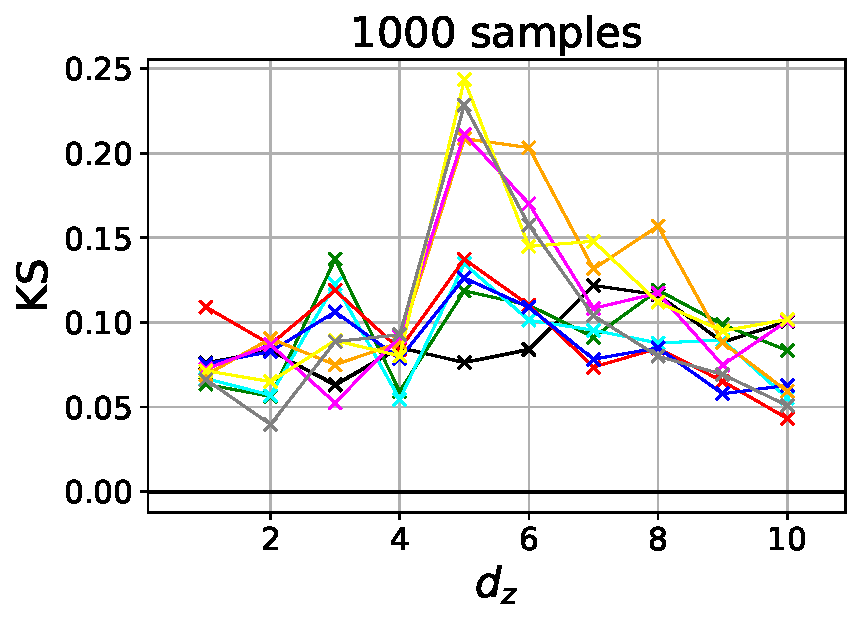
\includegraphics[height=3.7cm]{sections/appendix/independence_testing_kernel/figures_J_p/fig_ours_J_p_ks.pdf}& 
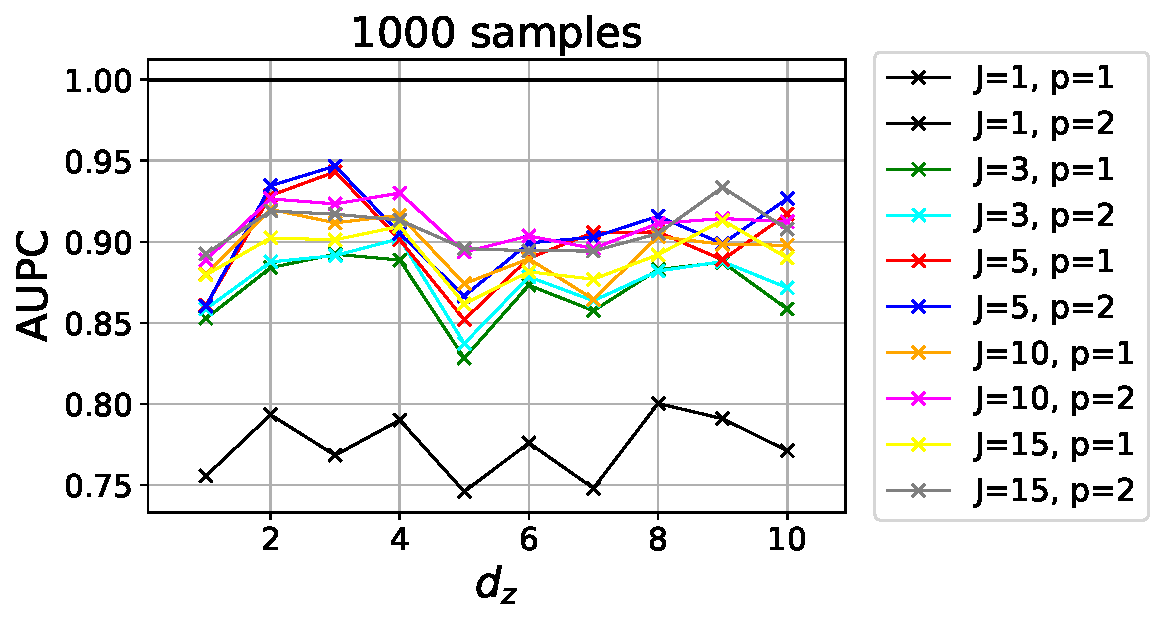
\includegraphics[height=3.7cm]{sections/appendix/independence_testing_kernel/figures_J_p/fig_ours_J_p_aupc.pdf}
\end{tabular}
\caption{Comparison of the KS statistic (\emph{left}) and the AUPC (\emph{right}) of our test statistic $\widetilde{\text{NCI}}_{n,r,p}$ when the data is generated respectively from the models defined in~\eqref{exp-strobl-h0} and~\eqref{exp-strobl-h1} with Gaussian noises for multiple $p$ and $J$. For each problem, we draw $n=1000$ samples and repeat the experiment 100 times. We set $r=1000$ and report the results obtained when varying the dimension $d_z$ of each problem from 1 to 10. Observe that when $J=1$, for all $p\geq 1$ $\widetilde{\text{NCI}}_{n,r,1}=\widetilde{\text{NCI}}_{n,r,p}$, therefore there is only one  common black curve.
\label{fig-exp-param}}
\vspace{-0.4cm}
\end{figure}

\begin{figure}[ht]
\begin{tabular}{cc} 
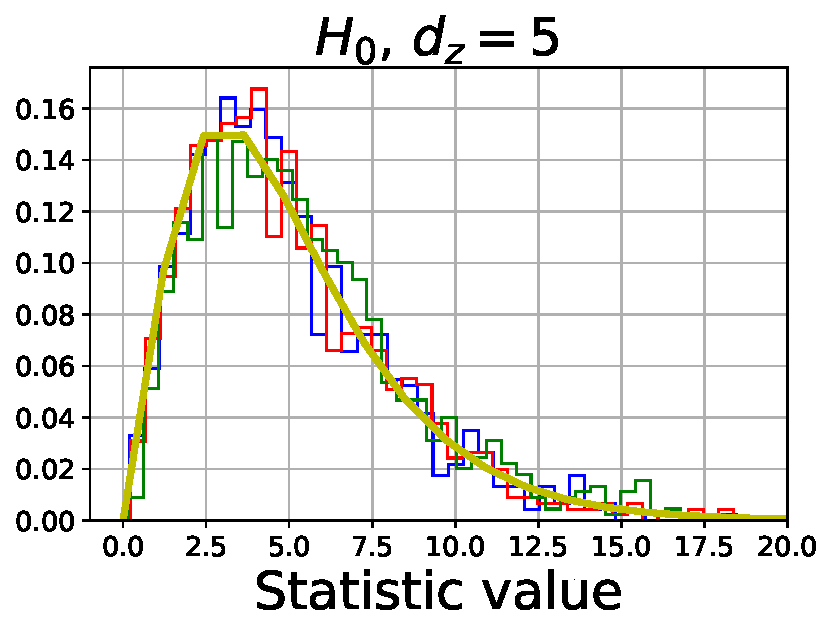
\includegraphics[width=0.24\textwidth]{sections/appendix/independence_testing_kernel/new_figures_oracle/oracle_h0_dim_5.pdf} 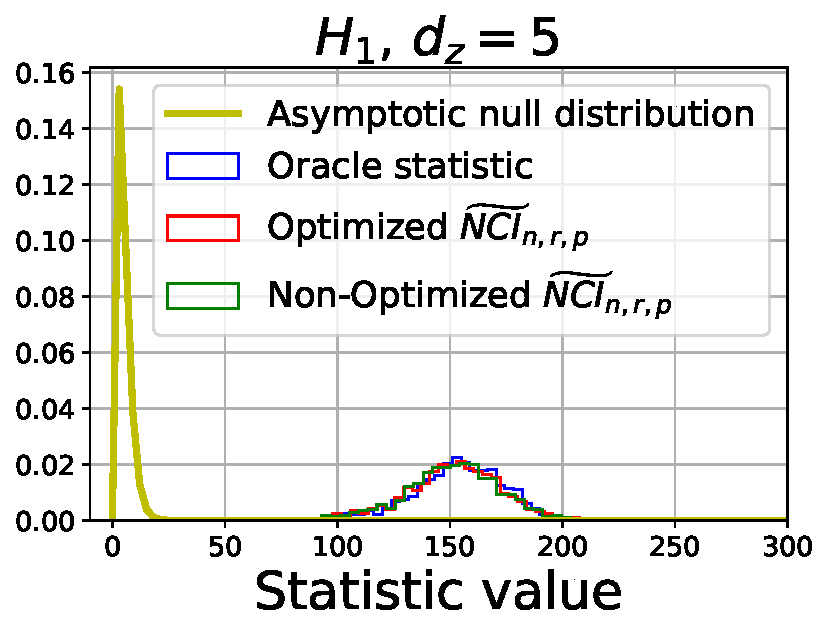
\includegraphics[width=0.24\textwidth]{sections/appendix/independence_testing_kernel/new_figures_oracle/oracle_h1_dim_5.pdf}  
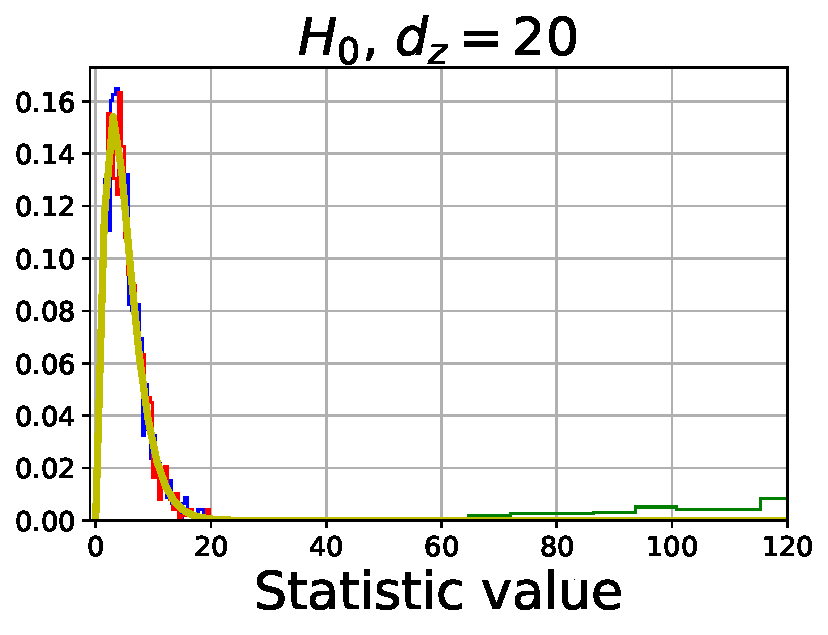
\includegraphics[width=0.24\textwidth]{sections/appendix/independence_testing_kernel/new_figures_oracle/oracle_h0_dim_20.pdf} 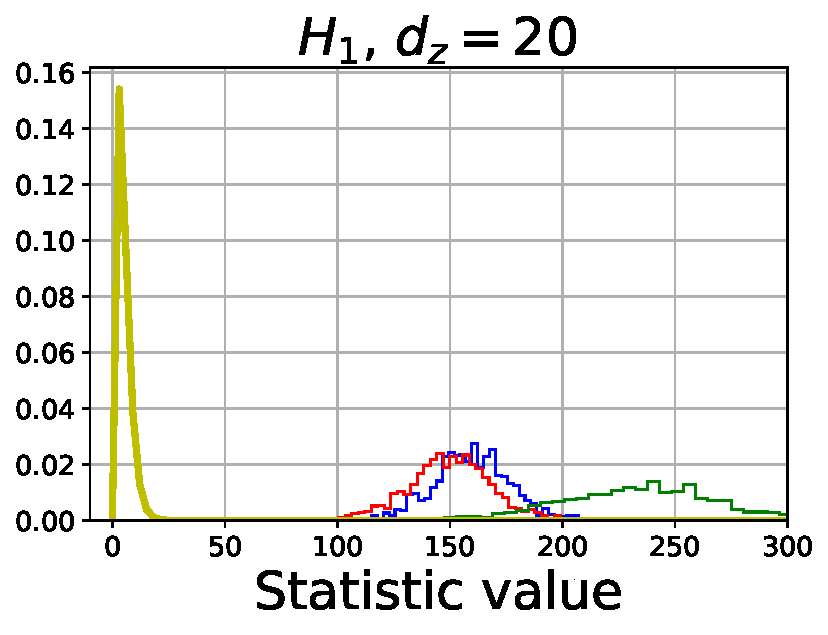
\includegraphics[width=0.24\textwidth]{sections/appendix/independence_testing_kernel/new_figures_oracle/oracle_h1_dim_20.pdf}
\end{tabular} 
\caption{Comparisons between the empirical distributions of the normalized version of the oracle statistic  $\widehat{\text{CI}}_{n,p}$ and the approximate normalized statistic $\widetilde{\text{NCI}}_{n,r,p}$, with the theoretical asymptotic null distribution when the data is generated either from the model defined in~\eqref{exp-illustration-h0} (\emph{left}) or the one defined in~\eqref{exp-illustration-h1} (\emph{right}). We set the dimension of $Z$ to be either $d_z=5$ (\emph{top row}) or $d_z=20$ (\emph{bottom row}). For each problem, we draw $n=1000$ samples and repeat the experiment 1000 times. In all the experiments, we set $J=5$ and $p=2$, thus the asymptotic null distribution follows a $\chi^2(5)$. Observe that both the oracle statistic and the approximated one recover the true asymptotic distribution under the null hypothesis. When $H_1$ holds, we can see that the two statistics manage to reject the null hypothesis. This figure also illustrates the empirical distribution of our approximate statistic when we do not optimize the hyperparameters involved in the RLS estimators: in this case we do not control the type-I error in the high dimensional setting.\label{fig-illustation-theory}}
\vspace{-0.4cm}
\end{figure}



% \begin{figure*}[tb]
% \begin{tabular}{cccc} 
% 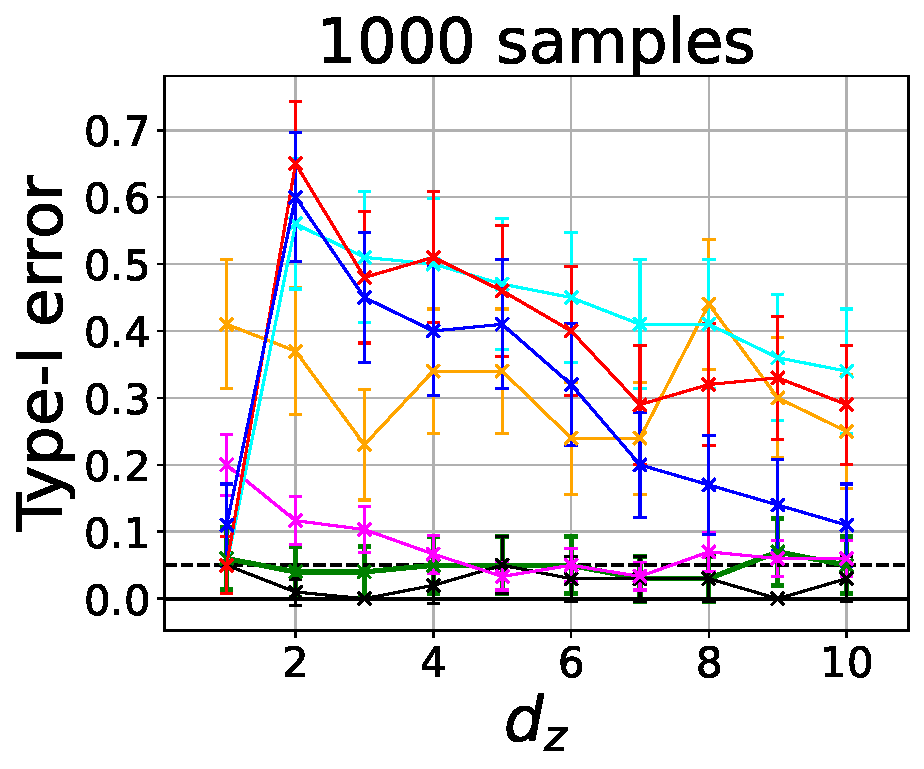
\includegraphics[height=3cm]{new_figures/nsamples_fixed_1000_li_dim_1_10_typeI.pdf}& 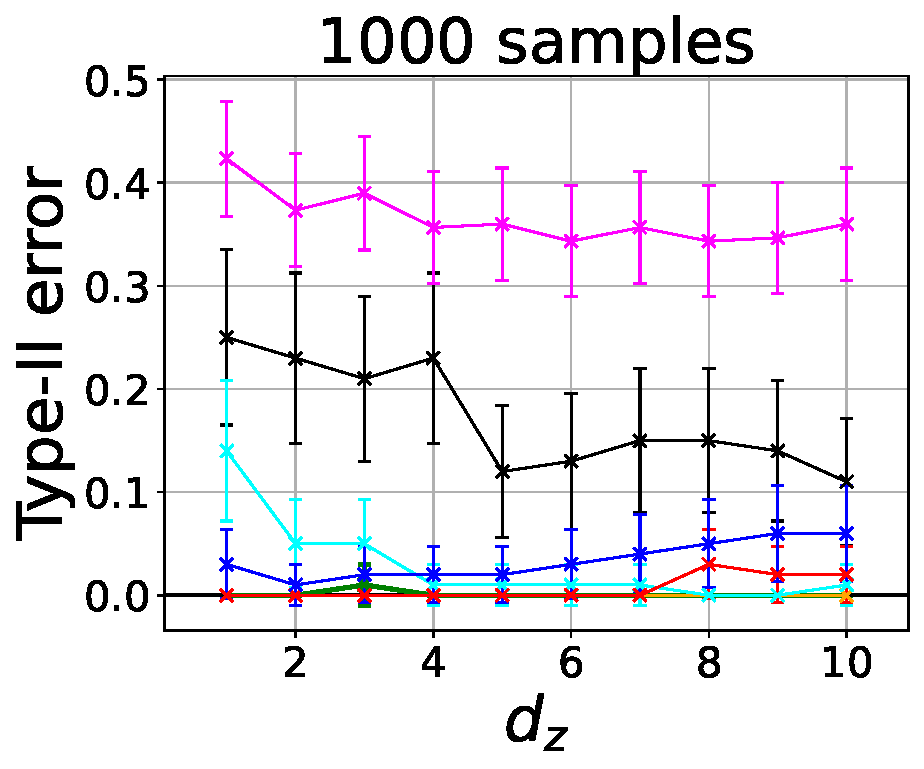
\includegraphics[height=3cm]{new_figures/nsamples_fixed_1000_li_dim_1_10_typeII.pdf} & 
% 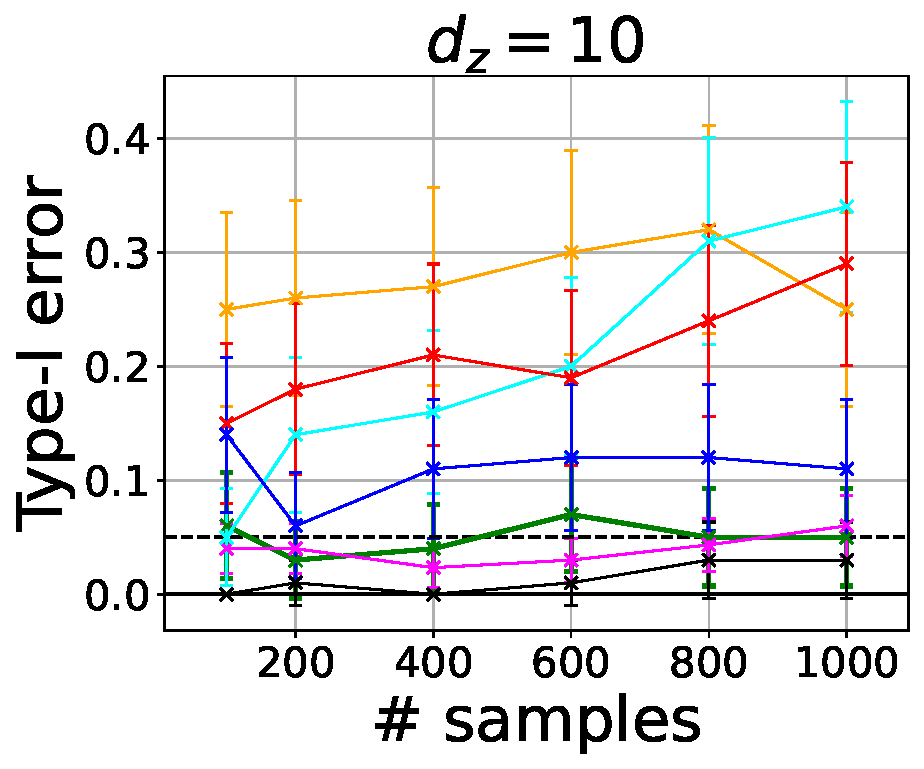
\includegraphics[height=3cm]{new_figures/dim_fixed_10_li_typeI.pdf}& 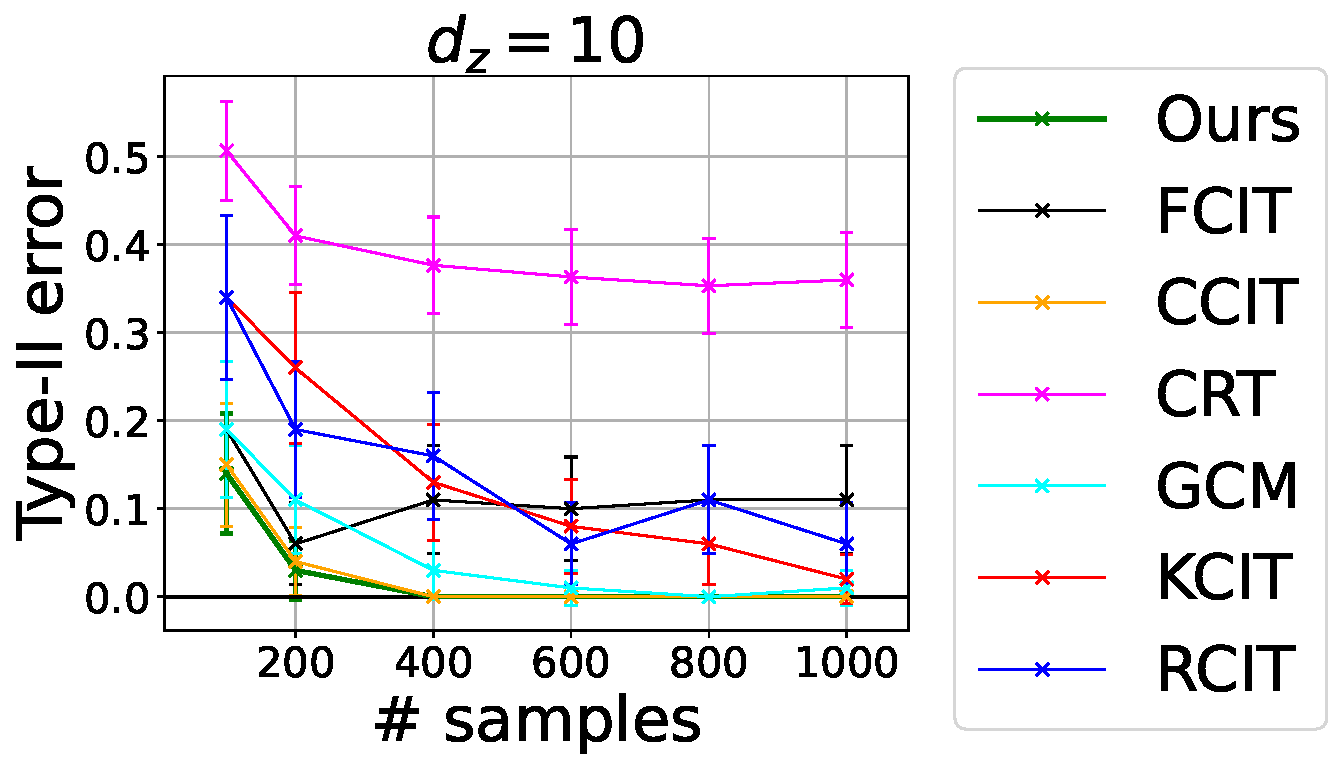
\includegraphics[height=3cm]{new_figures/dim_fixed_10_li_typeII.pdf} 
% \end{tabular}
% \caption{Comparison of the type-I error at level $\alpha=0.05$ (dashed line) and the type-II error (lower is better) of our test procedure with other SoTA tests on the two problems presented in~\eqref{li-exp-h0} and~\eqref{li-exp-h1}  with Gaussian noises. Each point in the figures is obtained by repeating the experiment for 100 independent trials. (\emph{Left, middle-left}): type-I and type-II errors obtained by each test when varying the dimension $d_z$ from 1 to 10; here, the number of samples $n$ is fixed and equals to $1000$. (\emph{Middle-right, right}): type-I and type-II errors obtained by each test when varying the number of samples $n$ from 100 to 1000; here, the dimension $d_z$ is fixed and equals to $10$. These experiments show that our method outperforms other tests as it manages to consistently control the type-I error and it is the most powerful. 
% \label{fig-exp-li}}
% \vspace{-0.3cm}
% \end{figure*}

% \begin{figure*}[ht]
% \begin{tabular}{cccc} 
% 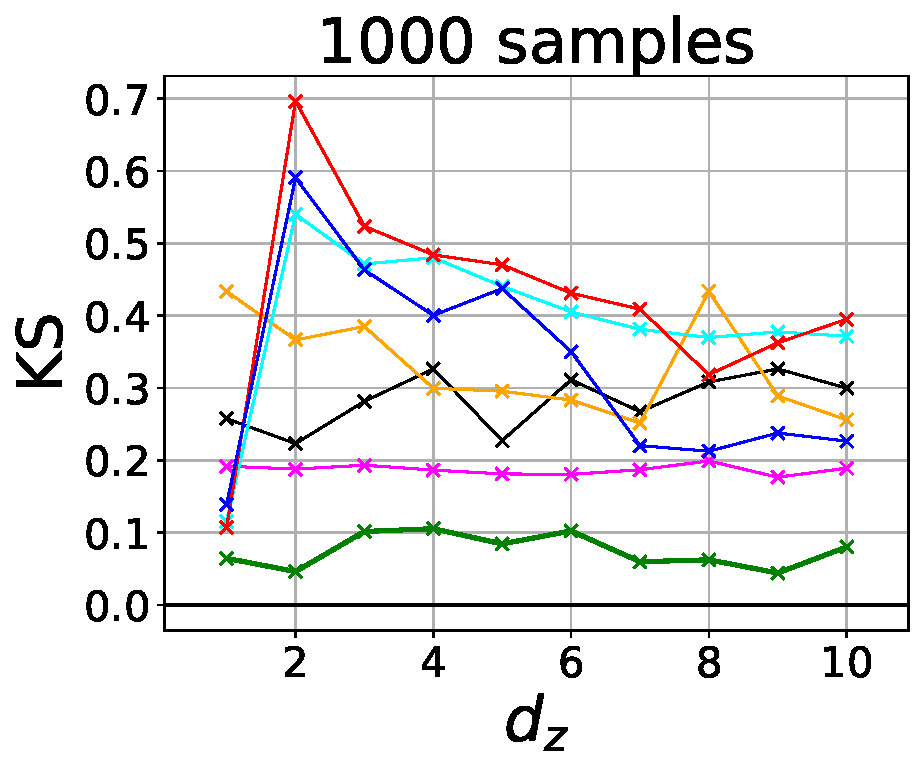
\includegraphics[height=2.3cm]{figures_supp_mat/nsamples_fixed_1000_li_dim_1_10_ks.pdf}& 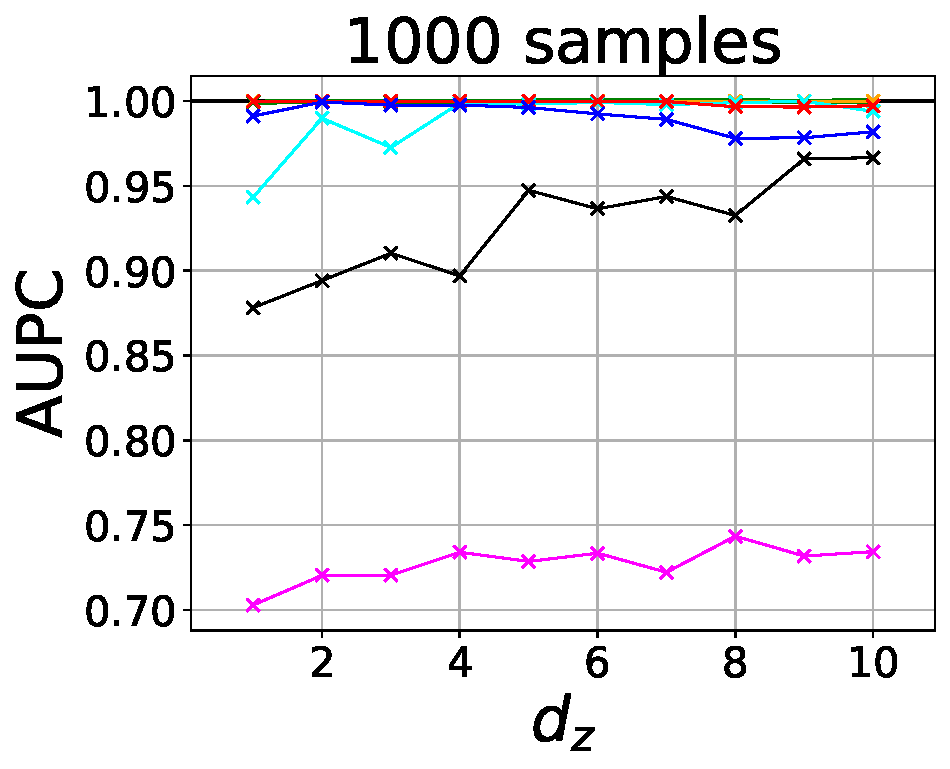
\includegraphics[height=2.3cm]{figures_supp_mat/nsamples_fixed_1000_li_dim_1_10_aupc.pdf} & 
% 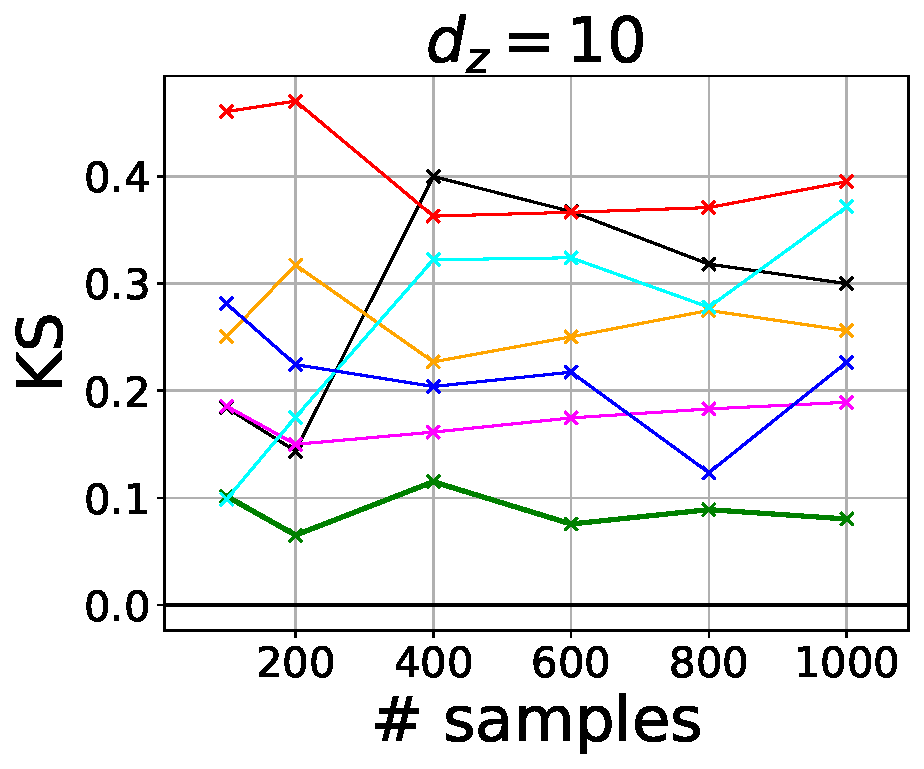
\includegraphics[height=2.3cm]{figures_supp_mat/dim_fixed_10_li_ks.pdf}& 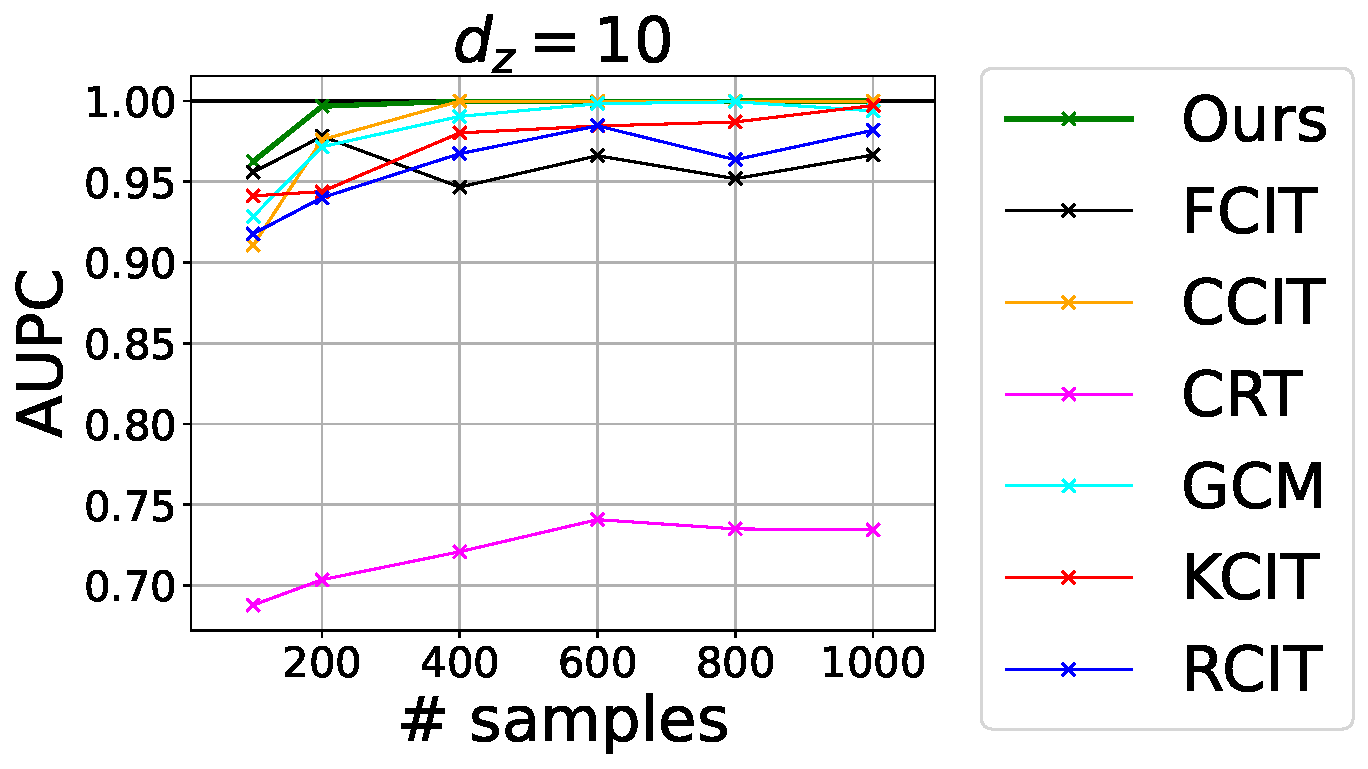
\includegraphics[height=2.3cm]{figures_supp_mat/dim_fixed_10_li_aupc.pdf}
% \end{tabular}
% \caption{Comparison of the KS statistic and the AUPC of our testing procedure with other SoTA tests on the two problems presented in Eq.~\eqref{li-exp-h0} and Eq.~\eqref{li-exp-h1} with Gaussian noises. Each point in the figures is obtained by repeating the experiment for 100 independent trials. (\emph{Left, middle-left}): the KS statistic and AUPC (respectively) obtained by each test when varying the dimension $d_z$ from 1 to 10; here, the number of samples $n$ is fixed and equals to $1000$. (\emph{Middle-right, right}): the KS and AUPC (respectively), obtained by each test when varying the number of samples $n$ from 100 to 1000; here, the dimension $d_z$ is fixed and equals to $10$.
% \label{fig-exp-li-ks}}
% \vspace{-0.3cm}
% \end{figure*}

\begin{figure*}[h]
\begin{tabular}{cccc} 
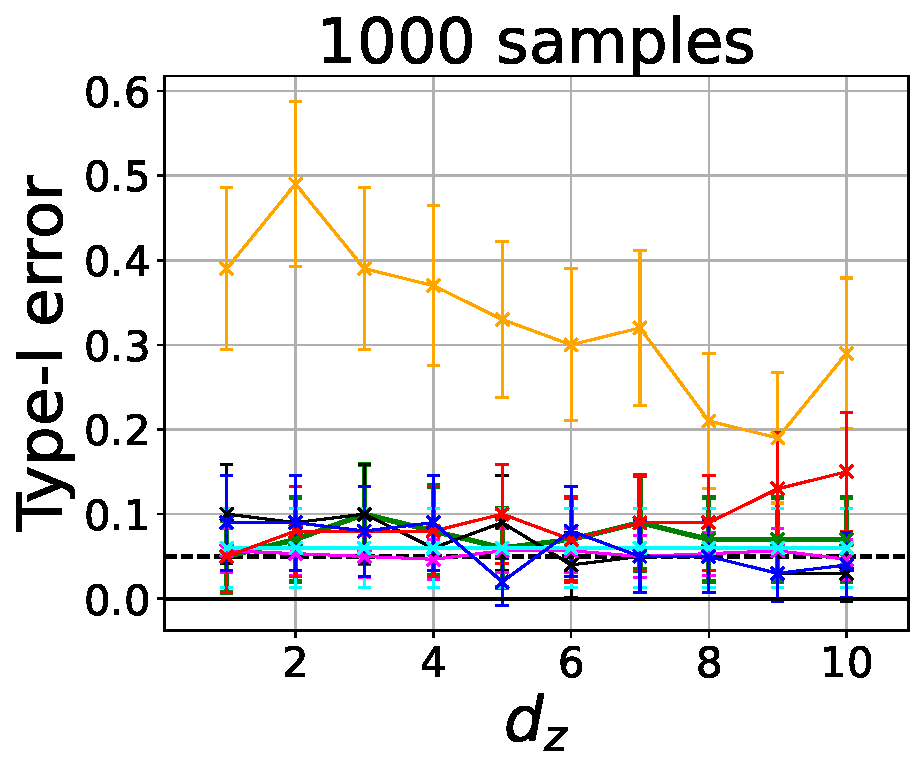
\includegraphics[height=2.3cm]{sections/appendix/independence_testing_kernel/figures_strobl_gaussian/nsamples_fixed_1000_strobl_dim_1_10_typeI.pdf}& 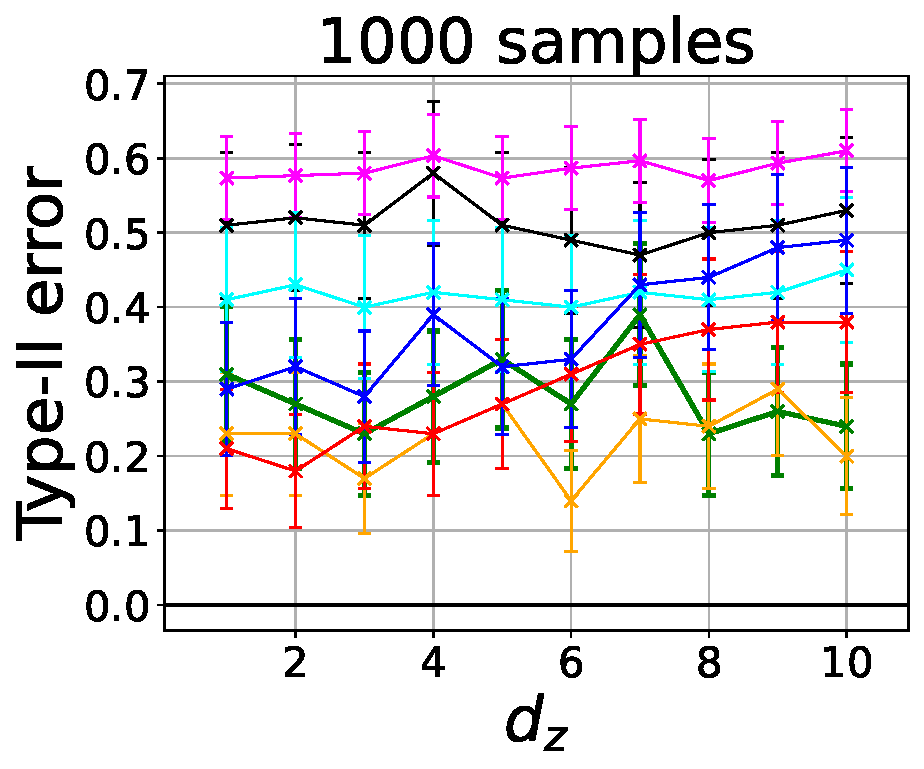
\includegraphics[height=2.3cm]{sections/appendix/independence_testing_kernel/figures_strobl_gaussian/nsamples_fixed_1000_strobl_dim_1_10_typeII.pdf} & 
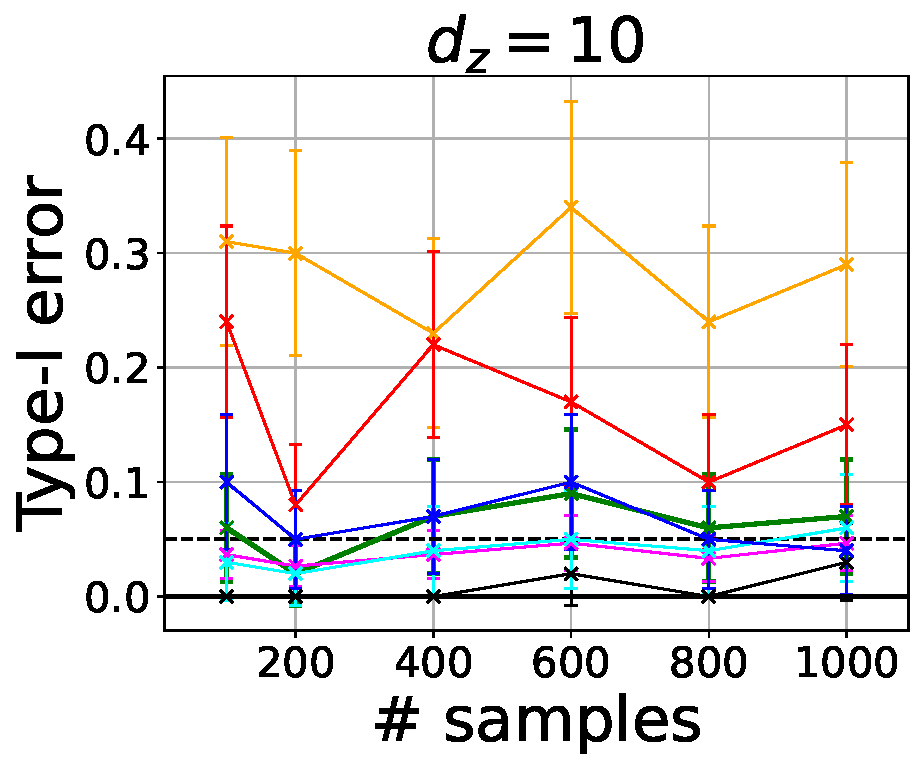
\includegraphics[height=2.3cm]{sections/appendix/independence_testing_kernel/figures_strobl_gaussian/dim_fixed_10_strobl_typeI.pdf}& 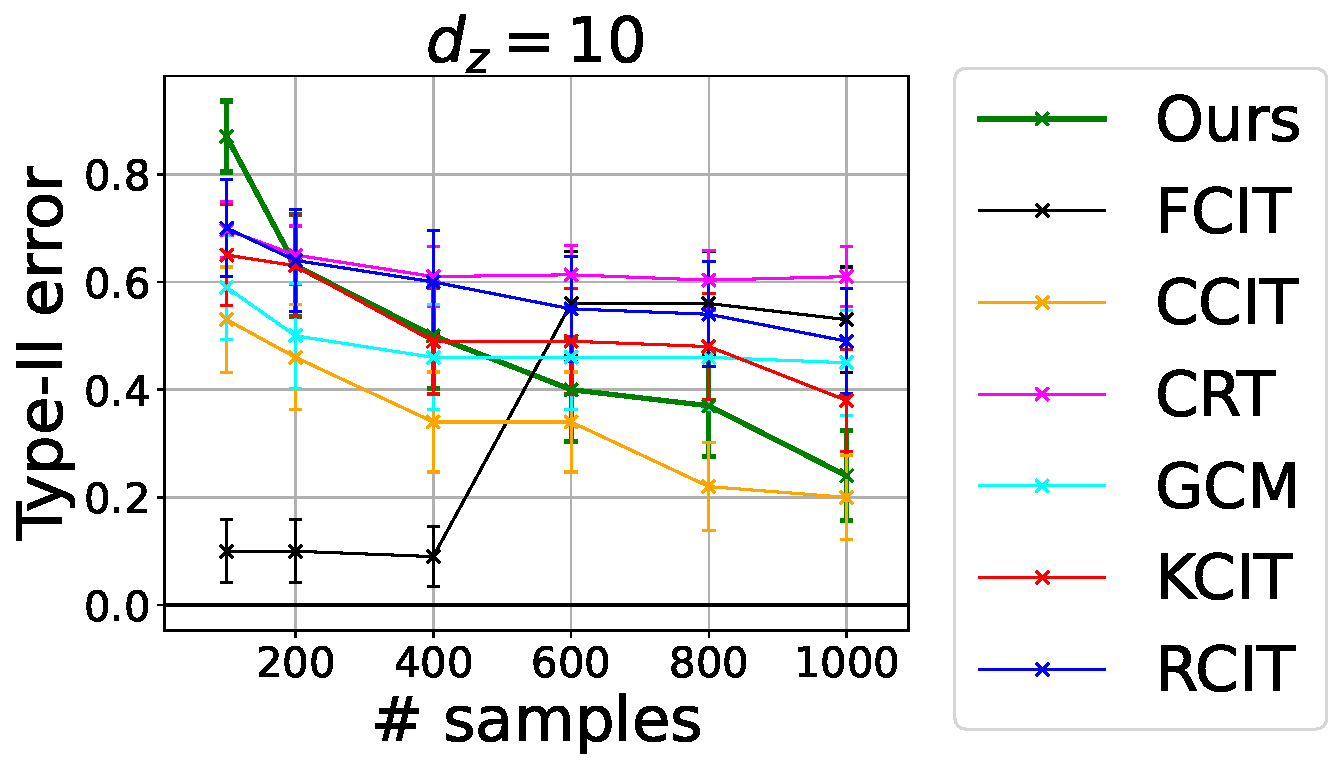
\includegraphics[height=2.3cm]{sections/appendix/independence_testing_kernel/figures_strobl_gaussian/dim_fixed_10_strobl_typeII.pdf}
\end{tabular}
\caption{Comparison of the type-I error at level $\alpha=0.05$ (dashed line) and the type-II error (lower is better) of our test procedure with other SoTA tests on the two problems presented in~\eqref{exp-strobl-h0} and~\eqref{exp-strobl-h1}  with Gaussian noises. Each point in the figures is obtained by repeating the experiment for 100 independent trials. (\emph{Left, middle-left}): type-I and type-II errors obtained by each test when varying the dimension $d_z$ from 1 to 10; here, the number of samples $n$ is fixed and equals to $1000$. (\emph{Middle-right, right}): type-I and type-II errors obtained by each test when varying the number of samples $n$ from 100 to 1000; here, the dimension $d_z$ is fixed and equals to $10$. 
\label{fig-exp-strobl-type}}
\vspace{-0.3cm}
\end{figure*}




The goal of this section is three fold: (i) to investigate the effects of the parameters $J$ and $p$ on the performances of our method, (ii) to validate our theoretical results depicted in Propositions~\ref{prop:oracle-law} and \ref{prop:norm-law}, and (iii) to compare our method with those proposed in the literature. In more detail, we first compare the performance of our method, both in terms of both power and type-I error, by varying the hyperparameters $J$ and $p$. We show that our method is robust to the choice of $p$, and also show that the power increases as $J$ increases. Then, we explore synthetic toy problems where one can derive an explicit formulation of the conditional means involved in our test statistic. In these cases, we can compute our proposed oracle statistic $\widehat{\text{CI}}_{n,p}$ and its normalized version, allowing us to show that under the null hypothesis we recover the theoretical asymptotic null distribution obtained in Proposition~\ref{prop:oracle-law}. We also reach to similar conclusions regarding our approximate normalized test statistic, $\widetilde{\text{NCI}}_{n,r,p}$. In addition, in this experiment, we investigate the effect of the proposed optimization procedure for choosing the hyperparameters involved in the RLS estimators of $\widetilde{\text{NCI}}_{n,r,p}$, and show its benefits. Finally, we demonstrate on several synthetic experiments that our proposed testing procedure outperforms state-of-the-art (SoTA) methods both in terms of statistical power and type-I error, even in the high dimensional setting. 




\textbf{Benchmarks.} We consider 6 synthetic data sets and compare the power and type-I error of our test $\widetilde{\text{NCI}}_{n,r,p}$ to the following 6 existing CI methods: \textbf{KCIT}~\citep{zhang2012kernel}, \textbf{RCIT}~\citep{strobl2019approximate}, \textbf{CCIT}~\citep{sen2017modelpowered}, \textbf{CRT}~\citep{candes2018panning} using correlation statistic from \citep{BellotS19}, \textbf{FCIT}~\citep{chalupka2018fast} and \textbf{GCM}~\citep{gcm2020}. Software packages of all the above tests are freely available online and each experiment was run on a single CPU. 





\textbf{Evaluation.} To evaluate the performance of the tests, we consider four metrics. Under $H_0$, we report either the Kolmogorov-Smirnov (KS) test statistic between the distribution of p-values returned by the tests and the uniform distribution on $[0,1]$, or the type-I errors at level $\alpha=0.05$. Note that a valid conditional independence test should control the type-I error rate at any level $\alpha$. Here, a test that generates a p-value that follows the uniform distribution over $[0,1]$ will achieve this requirement. The latter property of the p-values translates to a small KS statistic value. Under $H_1$, we compute either the area under the power curve (AUPC) of the empirical cumulative density function of the p-values returned by the tests, or the resulting type-II error. A conditional test has higher power when its AUPC is closer to one. Alternatively, the smaller the type-II error is, the more powerful the test is.

% \begin{figure*}[htb]
% \begin{tabular}{cccc} 
% 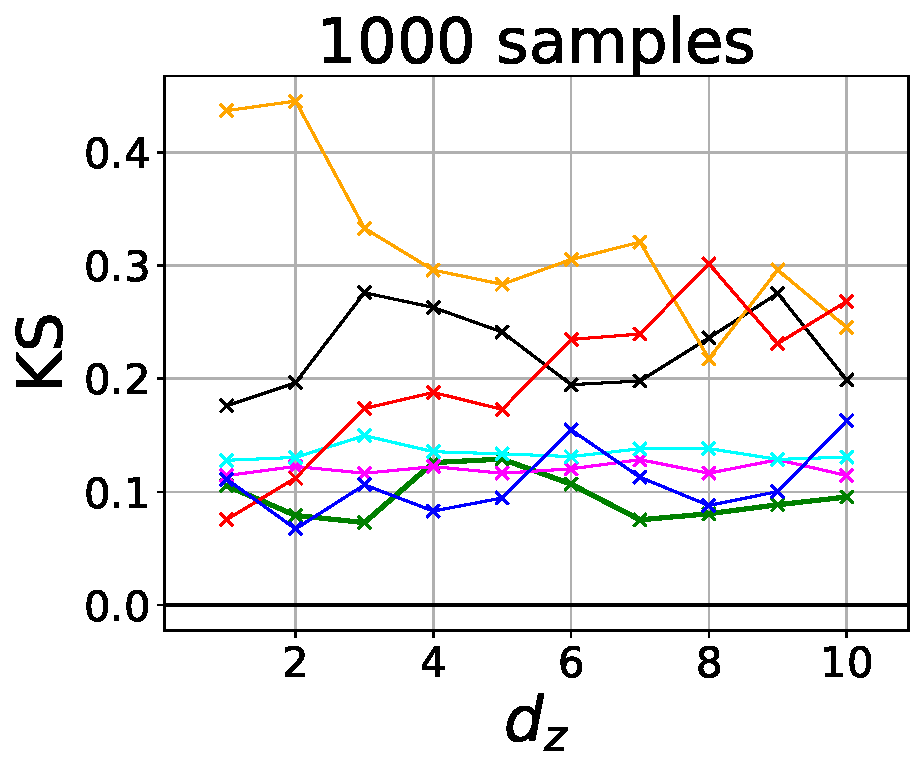
\includegraphics[height=2.3cm]{new_figures_lap/nsamples_fixed_1000_strobl_dim_1_10_ks.pdf}& 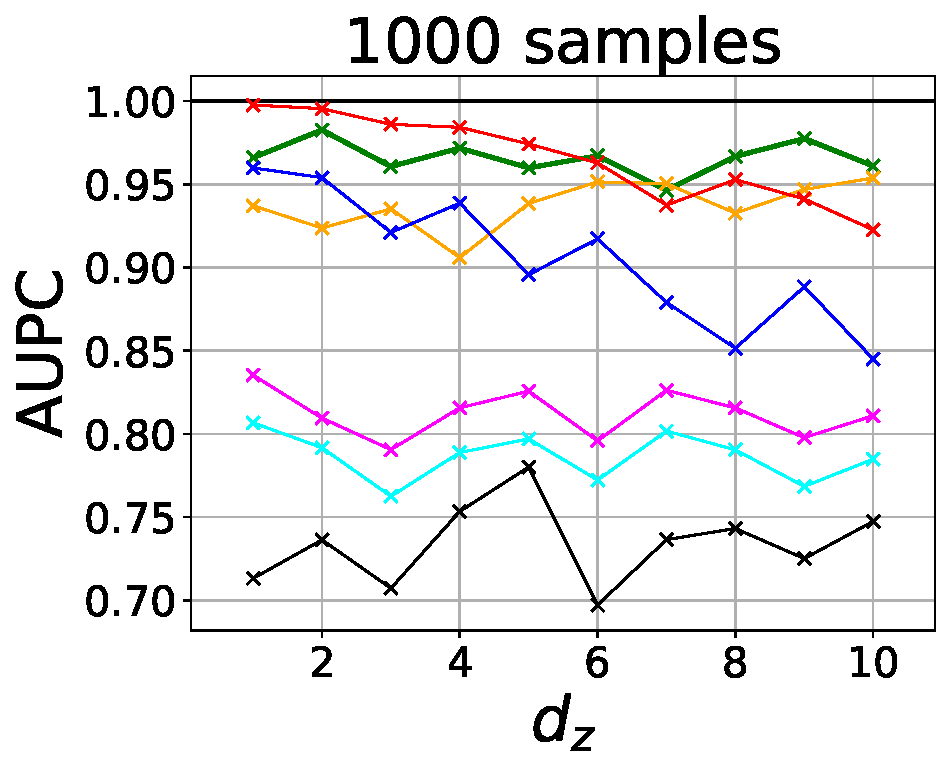
\includegraphics[height=2.3cm]{new_figures_lap/nsamples_fixed_1000_strobl_dim_1_10_aupc.pdf} & 
% 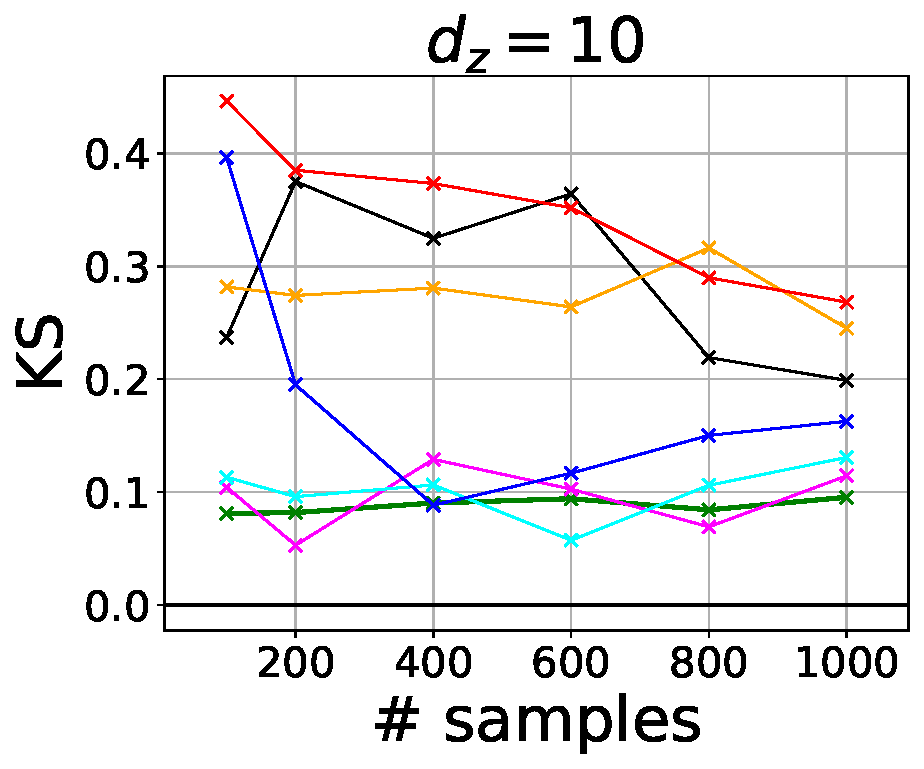
\includegraphics[height=2.3cm]{new_figures_lap/dim_fixed_10_strobl_ks.pdf}& 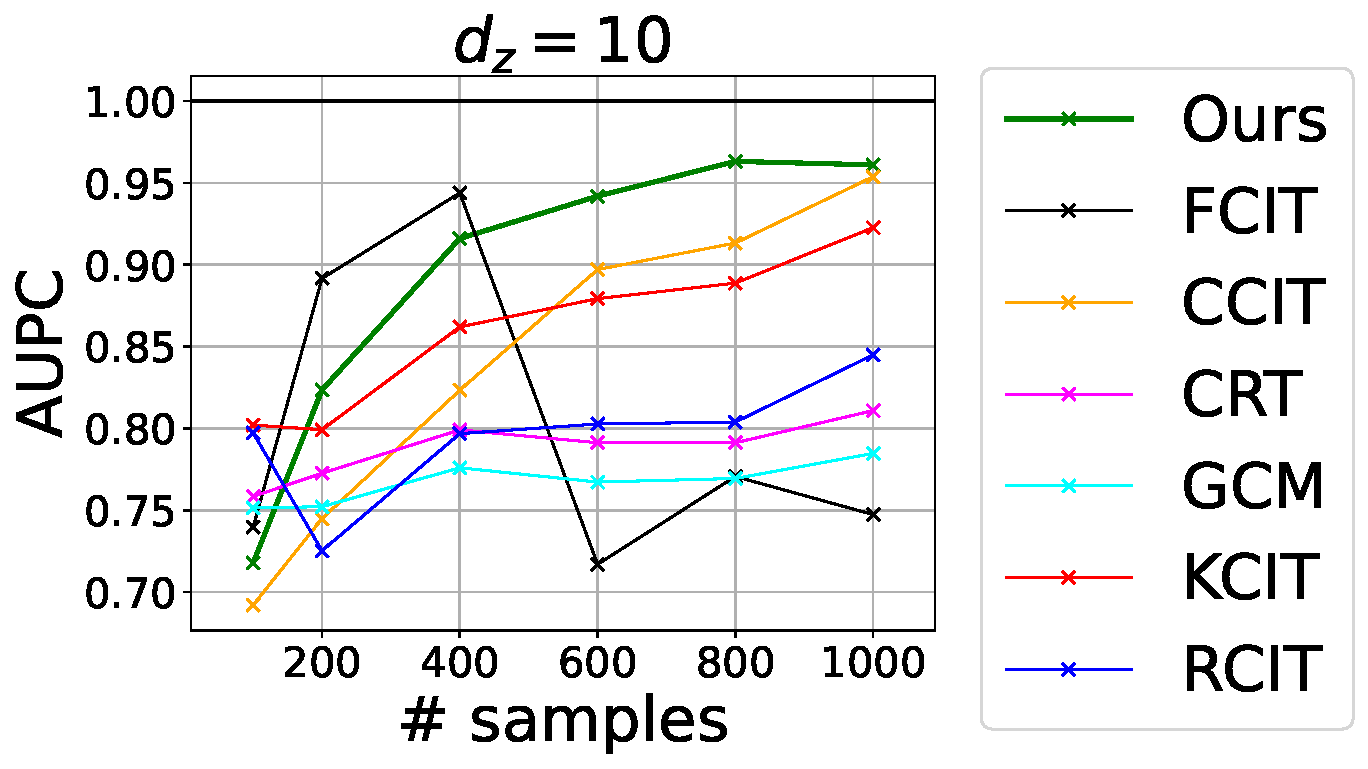
\includegraphics[height=2.3cm]{new_figures_lap/dim_fixed_10_strobl_aupc.pdf} 
% \end{tabular}
% \caption{Comparison of the KS statistic and the AUPC of our testing procedure with other SoTA tests on the two problems presented in Eq.~\eqref{exp-strobl-h0} and Eq.~\eqref{exp-strobl-h1}  with Laplace noises. Each point in the figures is obtained by repeating the experiment for 100 independent trials. (\emph{Left, middle-left}): the KS statistic and AUPC (respectively) obtained by each test when varying the dimension $d_z$ from 1 to 10; here, the number of samples $n$ is fixed and equals to $1000$. (\emph{Middle-right, right}): the KS and AUPC (respectively), obtained by each test when varying the number of samples $n$ from 100 to 1000; here, the dimension $d_z$ is fixed and equals to $10$.
% \label{fig-exp-strobl-ks-laplace}}
% \vspace{-0.3cm}
% \end{figure*}


\begin{figure*}[h]
\begin{tabular}{cccc} 
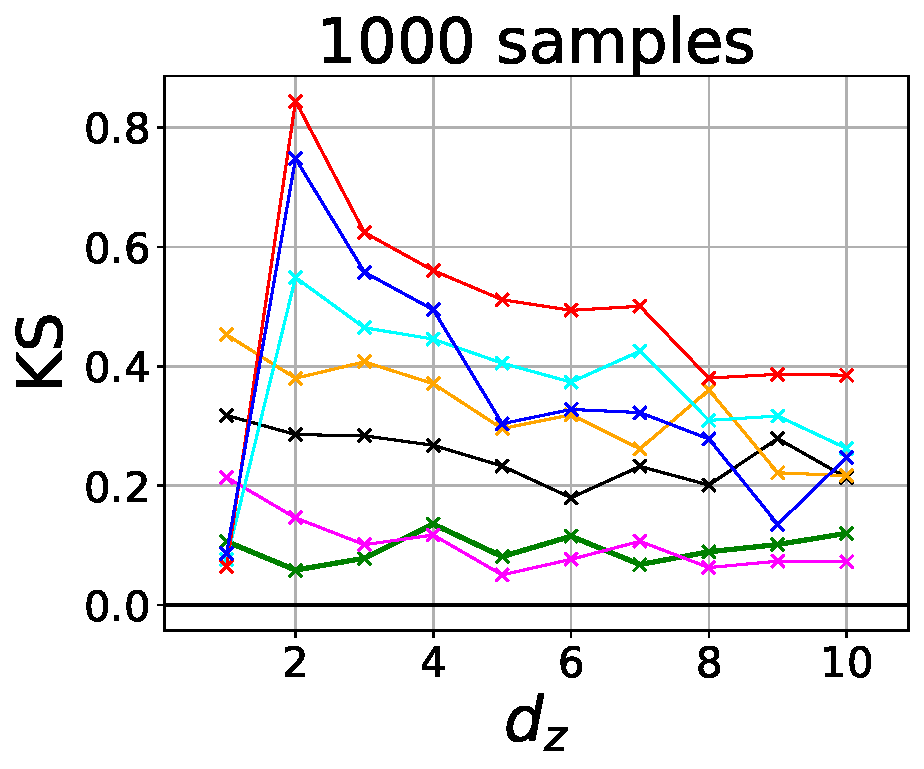
\includegraphics[height=2.3cm]{sections/appendix/independence_testing_kernel/new_figures_lap/nsamples_fixed_1000_li_dim_1_10_ks.pdf}& 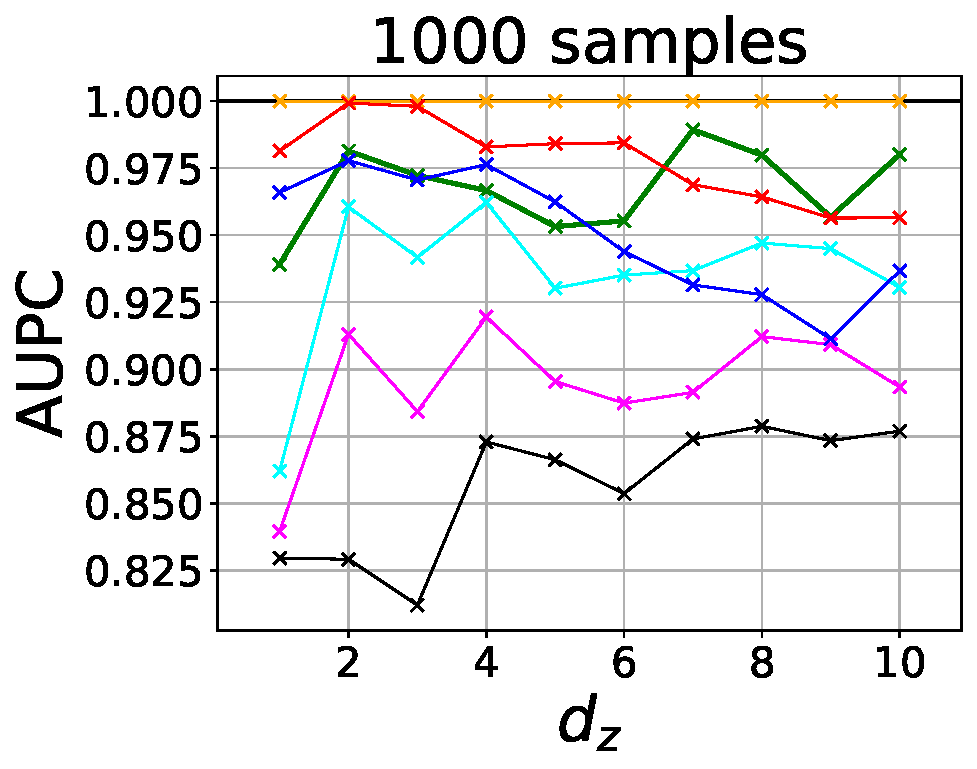
\includegraphics[height=2.3cm]{sections/appendix/independence_testing_kernel/new_figures_lap/nsamples_fixed_1000_li_dim_1_10_aupc.pdf} & 
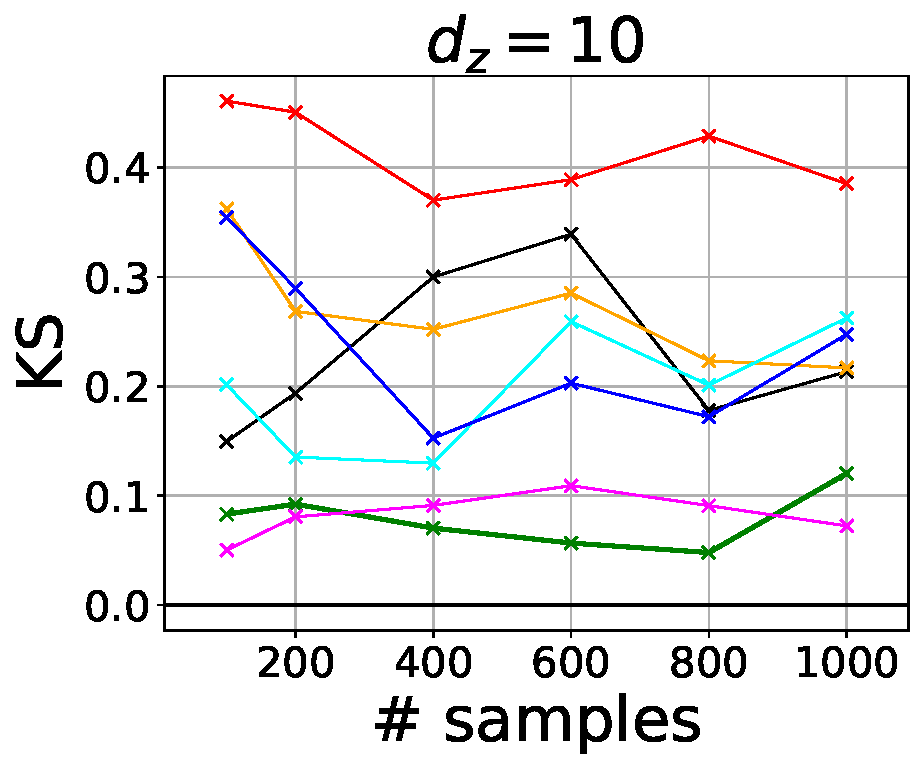
\includegraphics[height=2.3cm]{sections/appendix/independence_testing_kernel/new_figures_lap/dim_fixed_10_li_ks.pdf}& 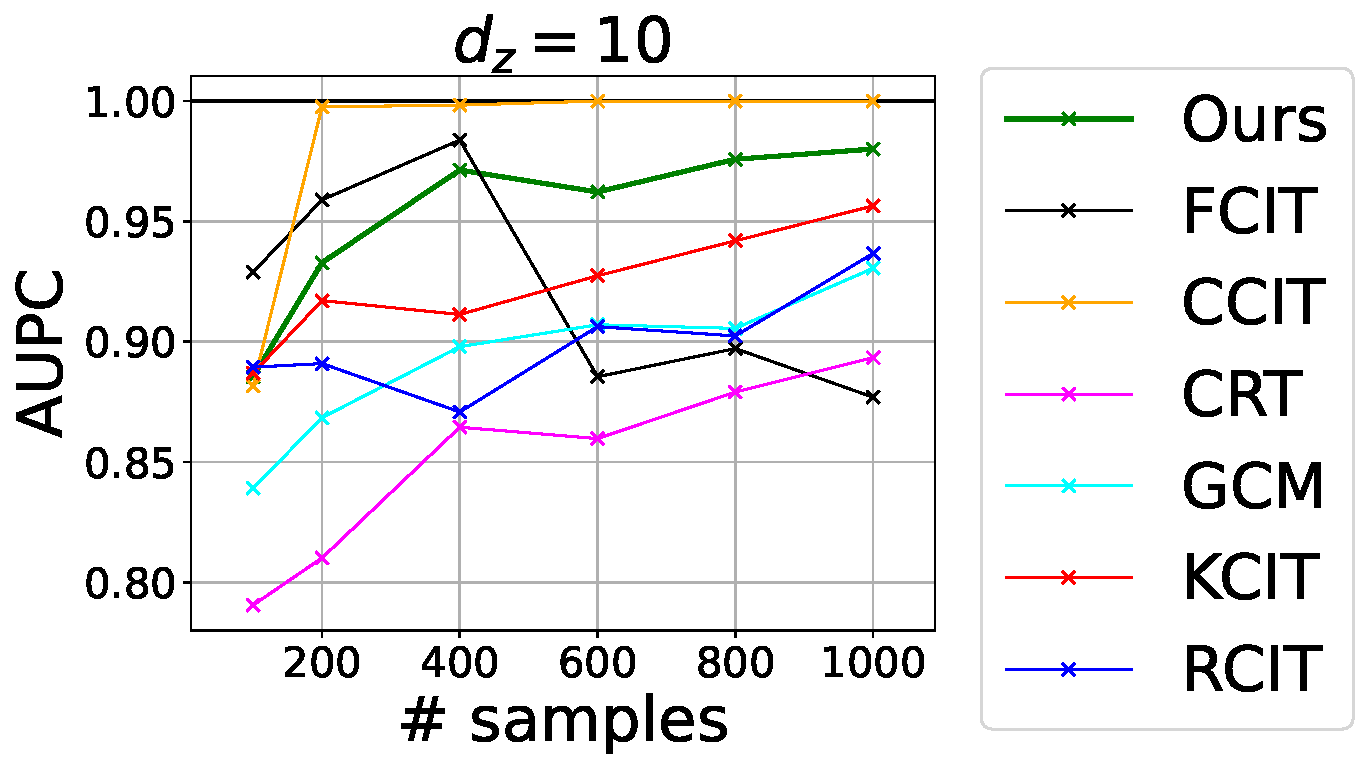
\includegraphics[height=2.3cm]{sections/appendix/independence_testing_kernel/new_figures_lap/dim_fixed_10_li_aupc.pdf} 
\end{tabular}
\caption{Comparison of the KS statistic and the AUPC of our testing procedure with other SoTA tests on the two problems presented in Eq.~\eqref{li-exp-h0} and Eq.~\eqref{li-exp-h1}  with Laplace noises. Each point in the figures is obtained by repeating the experiment for 100 independent trials. (\emph{Left, middle-left}): the KS statistic and AUPC (respectively) obtained by each test when varying the dimension $d_z$ from 1 to 10; here, the number of samples $n$ is fixed and equals to $1000$. (\emph{Middle-right, right}): the KS and AUPC (respectively), obtained by each test when varying the number of samples $n$ from 100 to 1000; here, the dimension $d_z$ is fixed and equals to $10$.
\label{fig-exp-li-ks-laplace}}
\vspace{-0.4cm}
\end{figure*}



\textbf{Effects of $p$, $J$ and $r$.} Our first experiment studies the effects of $p$ and $J$ on our proposed method. In addition we investigate the sensitivity of the method when varying the rank regression $r$ both in term of performance and time. To do so, we follow the synthetic experiment proposed in~\cite{strobl2019approximate}. To evaluate the type-I error, we generate data that follows the model:
\begin{align}
\label{exp-strobl-h0}
    X=f_1(\varepsilon_x), \ Y=f_2(\varepsilon_y),~\text{and Z}\sim\mathcal{N}(0_d,I_{d_z}),
\end{align}
where $Z$, $\varepsilon_x$, and $\varepsilon_y$ are samples from jointly independent standard Gaussian or Laplace distributions, and $f_1$ and $f_2$ are smooth
functions chosen uniformly from the set $\{(\cdot), (\cdot)^2, (\cdot)^3, \tanh(\cdot), \exp(-|\cdot|)\}$. To compare the power of the tests, we also consider the model:
\begin{align}
\label{exp-strobl-h1}
    X=f_1(\varepsilon_x +0.8\varepsilon_b), Y=f_2(\varepsilon_y+0.8\varepsilon_b),
\end{align}
where $\varepsilon_b$ is sampled from a standard Gaussian or Laplace distribution. In Figure~\ref{fig-exp-param}, we compare the KS statistic and the AUPC of our method when varying $p$ and $J$. That figure shows that (i) our method is robust to the choice of $p$, and (ii) the performances of the test do not necessarily increase as $J$ increases. In Figure~\ref{fig-rn-dependence} (see Appendix~\ref{sec-rank-rn}), we also show that the power of the test is not very sensible to the choice of the rank $r$, however, we observe that the type-I error decreases as the rank $r$ increases. Armed with theses observations, in the following experiments, we always set $p=2$, $J=5$ and $r=n$ for our method.


\textbf{Illustrations of our theoretical findings.} 
The following experiment confirms that validity of our theoretical results from Propositions~\ref{prop:oracle-law} and \ref{prop:norm-law}. For that purpose, we generate two synthetic data sets for which either $H_0$ or $H_1$ holds. Concretely, we define a first triplet $(X,Y,Z)$ as follows:
\begin{align}
\label{exp-illustration-h0}
X = \text{P}_1(Z) + \varepsilon_x,~~Y = \text{P}_1(Z) + \varepsilon_y.
\end{align}
Above, $\varepsilon_x$ and $\varepsilon_y$ follow two independent standard normal distributions, $Z\sim \mathcal{N}(0_{d_z},\Sigma)$ with $\Sigma\in\mathbb{R}^{d_z\times d_z}$. The covariance matrix $\Sigma$  is obtained by multiplying product of a random matrix whose entries are independent and follow standard normal distribution, by its transpose, and $\text{P}_1$ is a projection onto the first coordinate. As a result, in this case, we have that $X\perp Y \mid Z$. We also consider a modification of the above data generating function for which $H_1$ holds. This is done by adding a noise component $\varepsilon_b$ that is shared across $X$ and $Y$ as follows:
\begin{align}
\label{exp-illustration-h1}
X = \text{P}_1(Z) + \varepsilon_x + \varepsilon_b,~~ Y = \text{P}_1(Z) + \varepsilon_y + \varepsilon_b,
\end{align}
where $\varepsilon_b$ follows the standard normal distribution. Since we consider \emph{Gaussian kernels}, we can obtain an explicit formulation of $\mathbb{E}_{\ddot{X}}\left[k_{\mathcal{\ddot{X}}}(\mathbf{t}^{(1)}_j,\ddot{X})|Z=\cdot\right]$ and $\mathbb{E}_{Y}\left[k_{\mathcal{Y}}(t^{(2)}_j,Y)|Z=\cdot\right]$ for both data generation functions. See Appendix~\ref{sec-theoritical-findings} for more details. 
Consequently, we are able to compute both the normalized version of our oracle statistic $\widehat{\text{CI}}_{n,p}$ and our approximate normalized statistic $\widetilde{\text{NCI}}_{n,r,p}$. In Figure~\ref{fig-illustation-theory}, we show that both statistics manage to recover the asymptotic distribution under $H_0$, and reject the null hypothesis under $H_1$. In addition, we show that in the high dimensional setting, only our optimized version of $\widetilde{\text{NCI}}_{n,r,p}$---obtained by optimizing the hyperparameters involved in the RLS estimators of our statistic---manages to recover the asymptotic distribution under $H_0$.





\textbf{Comparisons with existing tests.} In our next experiments, we compare the performance of our method (implemented with the optimized version of our statistic) with state-of-the-art techniques for conditional independence testing. We first study the two data generating functions from \eqref{exp-strobl-h0} and \eqref{exp-strobl-h1}. For each of these problems, we consider two settings. In the first, we fix the dimension $d_z$ while varying the number of samples $n$. In the second, we fix the number of samples while varying the dimension of the problem. To evaluate the performance of the tests, we compare the type-I errors at level $\alpha=0.05$ under the first model~\eqref{exp-strobl-h0}, and, for second model~\eqref{exp-strobl-h1}, we evaluate the power of the test by presenting the type-II error. Figures~\ref{fig-exp-strobl-type} (Gaussian case) and \ref{fig-exp-strobl-laplace-supp} (Laplace case) demonstrate that our method consistently controls the type-I error and obtains a power similar to the best SoTA tests. In Figures~\ref{fig-exp-strobl-ks-supp} and \ref{fig-exp-strobl-ks-laplace-supp}, we also compare the KS statistic and the AUPC of the different tests, and obtain similar conclusions. In addition, we investigate the high dimensional regime and show in Figure~\ref{fig-exp-strobl-highdim-gaussian-supp} and \ref{fig-exp-strobl-highdim-laplace-supp} that our test is the only one which manages to control the type-I error while being competitive in term of power with other methods. See Appendix~\ref{sec-exp-storbl} for more details. 


We now conduct another series of experiments that build upon the synthetic data sets presented in~\citep{zhang2012kernel,li2020nonparametric,doran2014permutation,BellotS19}.
To compare type-I error rates, we generate simulated data for which $H_0$ is true:
\begin{align}
\label{li-exp-h0}
X=f_1\left(\bar{Z}+\varepsilon_x\right),Y=f_2\left(\bar{Z}+\varepsilon_y\right).
\end{align}
Above, $\bar{Z}$ is the average of $Z=(Z_1,\cdots,Z_{d_z})$, $\varepsilon_x$ and $\varepsilon_y$ are sampled independently from a standard Gaussian or Laplace distribution, and $f_1$ and $f_2$ are smooth
functions chosen uniformly from the set $\{(\cdot), (\cdot)^2, (\cdot)^3, \tanh(\cdot), \exp(-|\cdot|)\}$. To evaluate the power, we consider the following data generating function:
\begin{align}
\begin{aligned}
\label{li-exp-h1}
 X=f_1\left( \bar{Z}+\varepsilon_x\right)+\varepsilon_b,Y=f_2\left(\bar{Z}+\varepsilon_y\right)+\varepsilon_b,
\end{aligned}
\end{align}
where $\varepsilon_b$ is a standard Gaussian or Laplace distribution. 
% We now conduct another series of experiments that build upon the synthetic data sets presented in~\cite{strobl2019approximate}. To evaluate the type-I error, we generate data that follows the model:
% \begin{align}
% \label{exp-strobl-h0}
%     X=f_1(\varepsilon_x), \ Y=f_2(\varepsilon_y),~\text{and Z}\sim\mathcal{N}(0_d,I_{d_z}),
% \end{align}
% where $Z$,   $\varepsilon_x$, and $\varepsilon_y$ are samples from jointly independent standard Gaussian or Laplace distributions depending on the experiment, and $f_1$ and $f_2$ are smooth
% functions chosen uniformly from the set $\{(\cdot), (\cdot)^2, (\cdot)^3, \tanh(\cdot), \exp(-|\cdot|)\}$. To compare the power of the tests, we also consider the model:
% \begin{align}
% \label{exp-strobl-h1}
%     X=f_1(\varepsilon_x +0.8\varepsilon_b), Y=f_2(\varepsilon_y+0.8\varepsilon_b),
% \end{align}
% where $\varepsilon_b$ is sampled from a standard Gaussian or Laplace distribution depending on the experiment. 
As in the previous experiment, for each model, we study two settings by either fixing the dimension $d_z$, or the sample size $n$. In Figure~\ref{fig-exp-li-ks-laplace} (Laplace case) and~\ref{fig-exp-li-ks-gauss-supp} (Gaussian case), we compare the KS and the AUPC of our method with the SoTA tests and demonstrate that our procedure manages to be powerful while controlling the type-I error. In Figures~\ref{fig-exp-li-type-supp} and \ref{fig-exp-li-laplace-supp}, we also compare the type-I and type-II errors of the different tests, and obtain similar conclusions. In addition, we investigate the high dimensional regime and show in Figure~\ref{fig-exp-li-highdim-gauss-supp} and \ref{fig-exp-li-highdim-laplace-supp} that our test outperforms all the other proposed methods in most of the settings. See Appendix~\ref{sec-exp-li} for more details.



% \paragraph{Real world experiment} Finally we test our procedure on a real world dataset. We reproduced the experiment of~\citep{BellotS19}. We use the subset of the CCLE data~\citep{barretina2012cancer} relating to the drug PLX4720; the dataset is composed 474 cancer cell lines described by 466 genetic mutations. As the ground truth causal links are unknown, effectively evaluating conditional dependence on real data is difficult .









% \subsection{Illustrations of our theoretical findings}
% Here we aim at illustrating our theoretical results obtained in Proposition~\ref{prop:rls-law} to show the distribution of our statistics under the null hypothesis. As in \citep{zhang2012kernel,doran2014permutation,BellotS19}, we generate synthetic data that follows the post non-linear noise model. Concretely, we define the triplet $(X,Y,Z)$ as follows:
% \begin{align*}
%     H_0:~& X = f(A_fZ + \varepsilon_f),\quad Y = g(A_gZ + \varepsilon_g)
% \end{align*}
% where $A_{f}, A_g$ and $A_h$ are vectors that result in univariate $X$ and $Y$. The entries in the three vectors and the parameter $\beta$ are all drawn from the $\text{Uniform}$ distribution on the $[0,1]$ interval. The noise parameters $\varepsilon_f, \varepsilon_g$, and $\varepsilon_h$ are sampled from the normal distribution with a zero mean and variance of $0.025$. The choice of the non-linear functions $f$ and $g$ affect the complexity of the statistical test. We follow \citep{BellotS19} and consider the case where $f=g=tanh$. We draw the entries of $Z$ from $\mathcal{N}(0,1)$. The number of samples considered is $n=1000$ and the dimension of the problems are $d_1=d_2=d_3=1$. As we have access to a closed expression of the density of the $\chi^2(J)$, we consider only the case when $p=2$ and we repeat $1000$ times the experiment in order to obtain the density of our statistics. In Figure~\ref{fig-asymptotic}, we plot the results obtained. We see that our measures converge quickly towards the $\chi^2(J)$ for all $J$, both when applying our RLS-based statistic and its random features relaxation.


% \begin{figure}[!h]
% \begin{center}
% 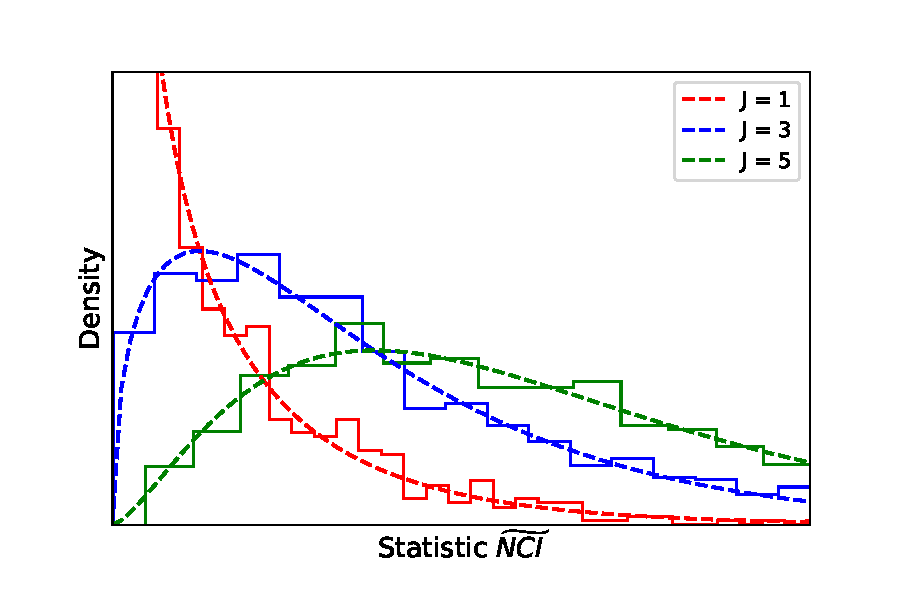
\includegraphics[width=0.45\textwidth]{figures/plot_density_2.pdf}
% 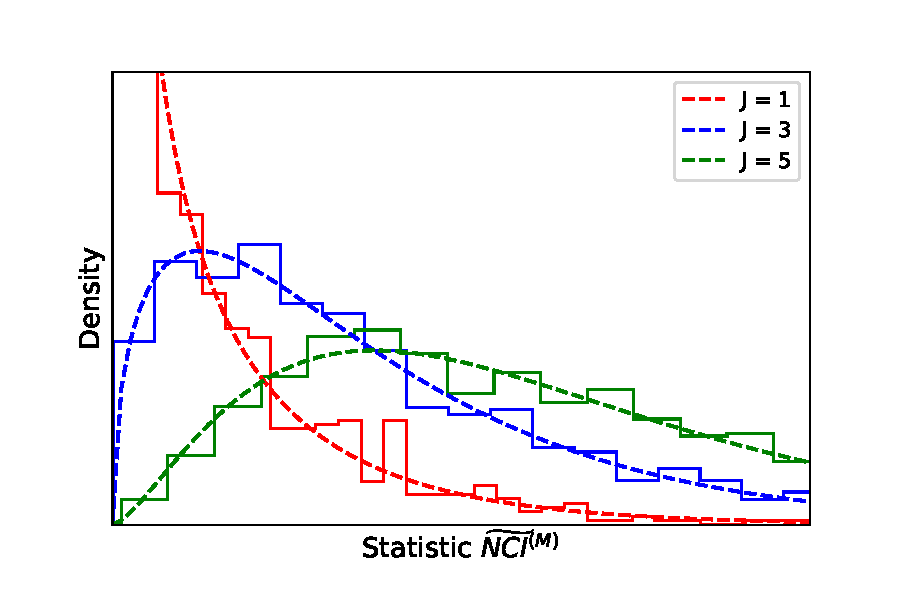
\includegraphics[width=0.45\textwidth]{figures/plot_density_rf_2.pdf}
% \caption{We show the distribution of our statistics for multiple choice of $J$. Here the number of random features is chosen to be $M=100$. Both statistics manage to reach the asymptotic regime of a the $\chi^2(J)$ distribution. \emph{(a)}: Distribution of the regularized least-squares based statistic $\widetilde{\text{NCI}}_{n,r,p}$ under the null hypothesis. \emph{(b)}: Distribution of the random features based statistic $\widetilde{\text{NCI}}^{(M)}_{n,r,p}$ under the null hypothesis. \label{fig-asymptotic}}
% \label{fig:couplings}
% \end{center}
% \vspace{-0.1cm}
% \end{figure}



% as well as the recently proposed conditional randomization test (CRT) \citep{candes2018panning}. The CRT is a powerful approach for conditional independence testing that allows the analyst to deploy any data-driven test statistic $T(\cdot)\in\mathbb{R}$---e.g., a summary statistic that builds upon a complex machine learning model---to examine the dependency structure of $X, Y$, and $Z$. The CRT test repeatedly generates dummy variables $\tilde{X}_i^k, \ 1 \leq i \leq n, \ 1 \leq k \leq K$ from the conditional null and compares the test statistic $T(\{Y_i\}_i,\{\tilde{X}_i\}_i,\{Z_i\}_i)$ to the one evaluated on the original data $T(\{Y_i\}_i,\{{X_i}\}_i,\{Z_i\}_i)$. The sampling from the conditional null is done by generating $\tilde{X}_i \sim P_{X \mid Z}(X \mid Z_i)$, and the p-value of the test is given by
% \begin{equation*}
%     p_{\text{CRT}} = \frac{1 + \sum_{i=1}^K \mathbf{1}\left\{t^* \leq T(\{Y_i\}_i,\{\tilde{X}_i^k\}_i,\{Z_i\}_i) \right\}}{K+1}.
% \end{equation*}
% Above, $t^* = T(\{Y_i\}_i,\{{X}\}_i,\{Z\}_i)$ is the statistic evaluated on the original data points.

% In practice, the conditional distribution $P_{X \mid Z}$---required to generate the dummy variables---is unknown. Following \citep{candes2018panning,BellotS19}, we use the observed data points to approximate the first two moments of this distribution. Importantly, the CRT may generate invalid p-values when provided with a poor approximation of $P_{X \mid Z}$. Indeed, recent methods, such as \citep{BellotS19, tansey2018holdout} attempt to move beyond the Gaussianity assumption and approximate $P_{X \mid Z}$ even for complex data sets.

% The choice of the test statistic affects the power of CRT. In our experiments, we examine several common scoring functions (see, e.g., \citep{BellotS19}), as listed below.
% \begin{itemize}
%     \item \textbf{CRT-Corr}: we set $T(\{Y_i\}_i,\{{X}\}_i,\{Z\}_i)$ to be the absolute value of the Pearson’s correlation coefficient between $\{X_i\}_i$ and $\{Y_i\}_i$.
%     \item \textbf{CRT-RDC}: we also examine the randomized dependence coefficient \citep{lopez2013randomized} as a measure of non-linear dependence between $\{X_i\}_i$ and $\{Y_i\}_i$.
 
%     \item \textbf{CRT-OLS}: this test statistic is obtained by (i) fitting an ordinary least squares model on the data, aiming to predict $\{Y_i\}_i$ from the pair $\{(X_i,Z_i)\}_i$, and (ii) returning the mean squared prediction error.
 
%     \item \textbf{CRT-KRidge}: in contrast to CRT-OLS, here we fit a kernel ridge regression model to the data, and then use the absolute value of the coefficient of determination (often denoted by $R^2$) as a summary statistic.
        
% \end{itemize}

% \subsection{Simulated data I}
% Here to test the the power of our method, we add to the previous setting a post nonlinear model where $H_1$ hold. More precisely we consider
% \begin{align*}
%     H_0:~& X = f(A_fZ + \varepsilon_f),\quad Y = f(A_gZ + \varepsilon_g) \\
%     H_1:~& Y=f(A_hZ + \beta X + \varepsilon_h),
% \end{align*}
% Moreover here $f$ is chosen among the following functions $\{x, x^2, \tanh{x}\}$. 

% % We compare our methods to KCIT, RCIT, CCIT, and GCIT.\footnote{We implemented KCIT and RCIT using the R package available at \url{https://github.com/ericstrobl/RCIT}. The software package of CCIT is from \url{https://github.com/rajatsen91/CCIT/blob/master/CCIT} and the one of GCIT is available at \url{https://github.com/alexisbellot/GCIT}. For all methods, we use the default set of hyper-parameters.} 


% In all experiments, we fix the number of samples $n$ to $600$ and increase the dimension of $Z$. Figure~\ref{fig:auc1}  compares the type-I error when testing $H_0$ at level $\alpha=0.05$ over 100 independent trials. As can be seen, all methods tend to control the type-I error, including our proposed tests. In Figure~\ref{fig:auc1} we compare the statistical power (higher is better) as a function of the dimension of $Z$. Observe how all the methods perform comparably well for in lower dimensions and depart as the dimensions increases. 

% \subsection{Simulated data II [This is the new data]}

% Following \citep{zhang2012kernel,doran2014permutation,BellotS19}, we generate synthetic data that follows the post non-linear noise model. Concretely, we define the triplet $(X,Y,Z)$ as follows:
% \begin{align*}
%     H_0:~& X = f(A_X Z + \varepsilon_x),\quad Y = f(A_Y Z + \varepsilon_y) \\
%     H_1:~& Y=f(A_Z Z + \beta X + \varepsilon_z),
% \end{align*}
% where $A_{X}, A_Y$ and $A_Z$ are vectors that result in univariate $X$ and $Y$, whose entries are drawn from the $\text{Uniform}(0,1)$ distribution. We set the dimension of $X$ to one and sample the parameter $\beta \in [0,1]$ from the uniform distribution as well. The noise parameters $\varepsilon_x, \varepsilon_y$, and $\varepsilon_z$ are sampled from a normal distribution with zero mean and variance that equals to $0.025$. 




% \begin{table}[]
% \centering
% \begin{tabular}{@{}ccc@{}}
% \toprule
% Setting & Distribution of $Z$                                                                        & Choice of $f$        \\ \midrule
% $H_0$: A  & \multirow{2}{*}{\begin{tabular}[c]{@{}c@{}}Gaussian\\ (mean 0, variance 1)\end{tabular}} & Identity: $f(x) = x$ \\
% $H_0$: B  &                                                                                          & Square: $f(x) = x^2$ \\ \midrule
% $H_0$: C  & \begin{tabular}[c]{@{}c@{}}Laplace\\ (location 0, scale 1)\end{tabular}                  & Identity: $f(x) = x$ \\ \bottomrule
% \end{tabular}
% \caption{Data generating mechanism under $H_0$.} \label{tab:data_H0}
% \end{table}

% The choice of the function $f$, the sampling distribution of the data, and the dimensions of the problem affect the complexity of test. In all experiments, we fix the number of samples $n$ to 600 and increase the dimension of $Z$ from 2 to 250. Table~\ref{tab:data_H0} summarizes three different settings that we examine when $H_0$ is true. 

% Figure ??? compares the type-I error of each method as a function of the dimension of $Z$. Here, we test the null hypothesis $H_0$ at level $\alpha=0.05$ by applying each test to 100 independent data sets. As can be seen, the tests we study tend to control the type-I error only when the dimension of 
% $Z$ is low, except the CRT that works well when the data follows the Gaussian distribution for which $f$ is the identity function. This is expected as we assume $X \mid Z$ to be Gaussian. When $Z$ follows the Laplace distribution, or when $f$ is the square function, the approximation we provide for the conditional distribution is poor, which, in turn, results in a violation of type-I error control. {\color{red} need to see the graphs}

% Next, we examine the power of the tests by generating data for which $H_1$ is true. We follow the same setting as described in Table~\ref{tab:data_H0}, except that now we also sampled $X$ from the same distribution of $Z$. In Figure ??? we plot the power of each test as a function of the dimension of $Z$. Observe how the ?????




% We compare our methods to KCIT, RCIT, CCIT, and GCIT.\footnote{We implemented KCIT and RCIT using the R package available at \url{https://github.com/ericstrobl/RCIT}. The software package of CCIT is from \url{https://github.com/rajatsen91/CCIT/blob/master/CCIT} and the one of GCIT is available at \url{https://github.com/alexisbellot/GCIT}. For all methods, we use the default set of hyper-parameters.} 


%  In Figure ??? we compare the statistical power (higher is better) as a function of the dimension of $Z$. Observe how all the methods perform comparably well for in lower dimensions and depart as the dimensions increases. ADD DETAILS WHEN GRAPHS WILL EXIST :)
    

% \subsection{Simulated data III}

% Herein, we generate synthetic data according to the following model:
% $$Y = f(X^{\top}\beta + \varepsilon ),$$
% where $X\in\mathbb{R}^{d}$ and the noise $\varepsilon \in\mathbb{R}$ is sampled independently from $\mathcal{N}(0,0.05)$. Above, the vector $X$ is generated by (i) independently sampling its entries from the standard Gaussian distribution, and (ii) applying the non-linear cosine function on each entry. We create the vector $\beta \in\mathbb{R}^{d}$ by assigning a non-zero value only in odd locations, where the magnitude of the $j$th non-zero is $1/j$. For example, for $d=7$ we have $\beta = [1, 0, 1/2, 0, 1/3, 0, 1/4]$. Under this construction, every odd coordinate $X_k \in \mathbb{R}$ is independent of $Y$ given $X_{-k} \in  \mathbb{R}^{d-1}$, where the latter is a vector that contains all the elements but the $k$th one. Analogously, every even coordinate $X_j$ is dependent of $Y$ given $X_{-j}$; here, as the index $j$ increases, the dependence is smaller and thus it is more challenging to detect that this variable departs from the null.




% \section{Discussions and conclusion}

% Our results on asymptotic distribution requires more assumptions than the results proposed by~\cite{zhang2012kernel}. Indeed, we need conditions to ensure the convergence rate of the RLS estimator. However, in~\citep{zhang2012kernel}, the proof of their asymptotic law requires assumptions to ours to hold. In~\citep{strobl1702approximate}, to prove their asymptotic distribution, the authors assume to have access to samples from the conditional mean, which is in practice impossible. In our work, by adding Assumptions~\ref{ass:spectrum}-\ref{ass:source}, we show we pr

% \begin{figure}
%     \centering
%     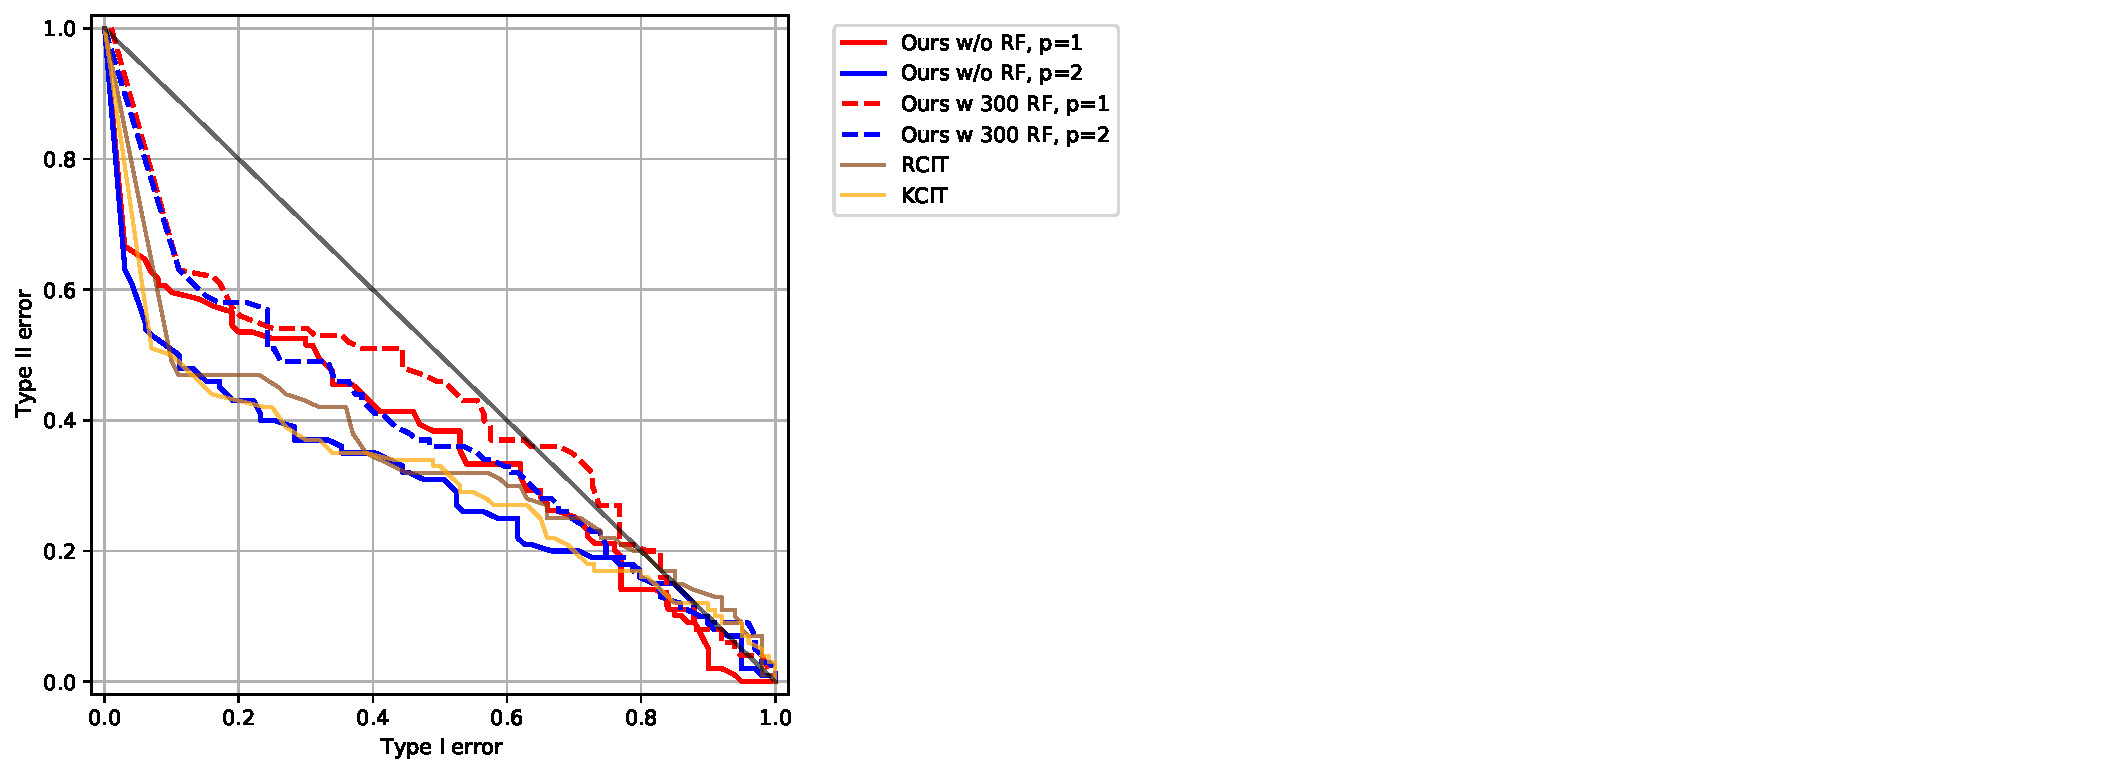
\includegraphics[width=0.85\textwidth]{figures/plots_v1_auc_5_True_square.pdf}
%     \caption{Area under curve comparing our approaches (Section~\ref{sec:42}) with KCIT and RCIT on a $5$ dimensional problem, with $f(x)=x^2$. The number of samples is fixed at $600$, and the results are averaged over $100$ runs. We chose $J=3$ and we optimized the positions of the $t_j$ and the parameters of the gaussian kernels. We fixed the rank of the RLS estimation to $r=300$.}
%     \label{fig:auc1}
% \end{figure}
% \begin{figure}
%     \centering
%     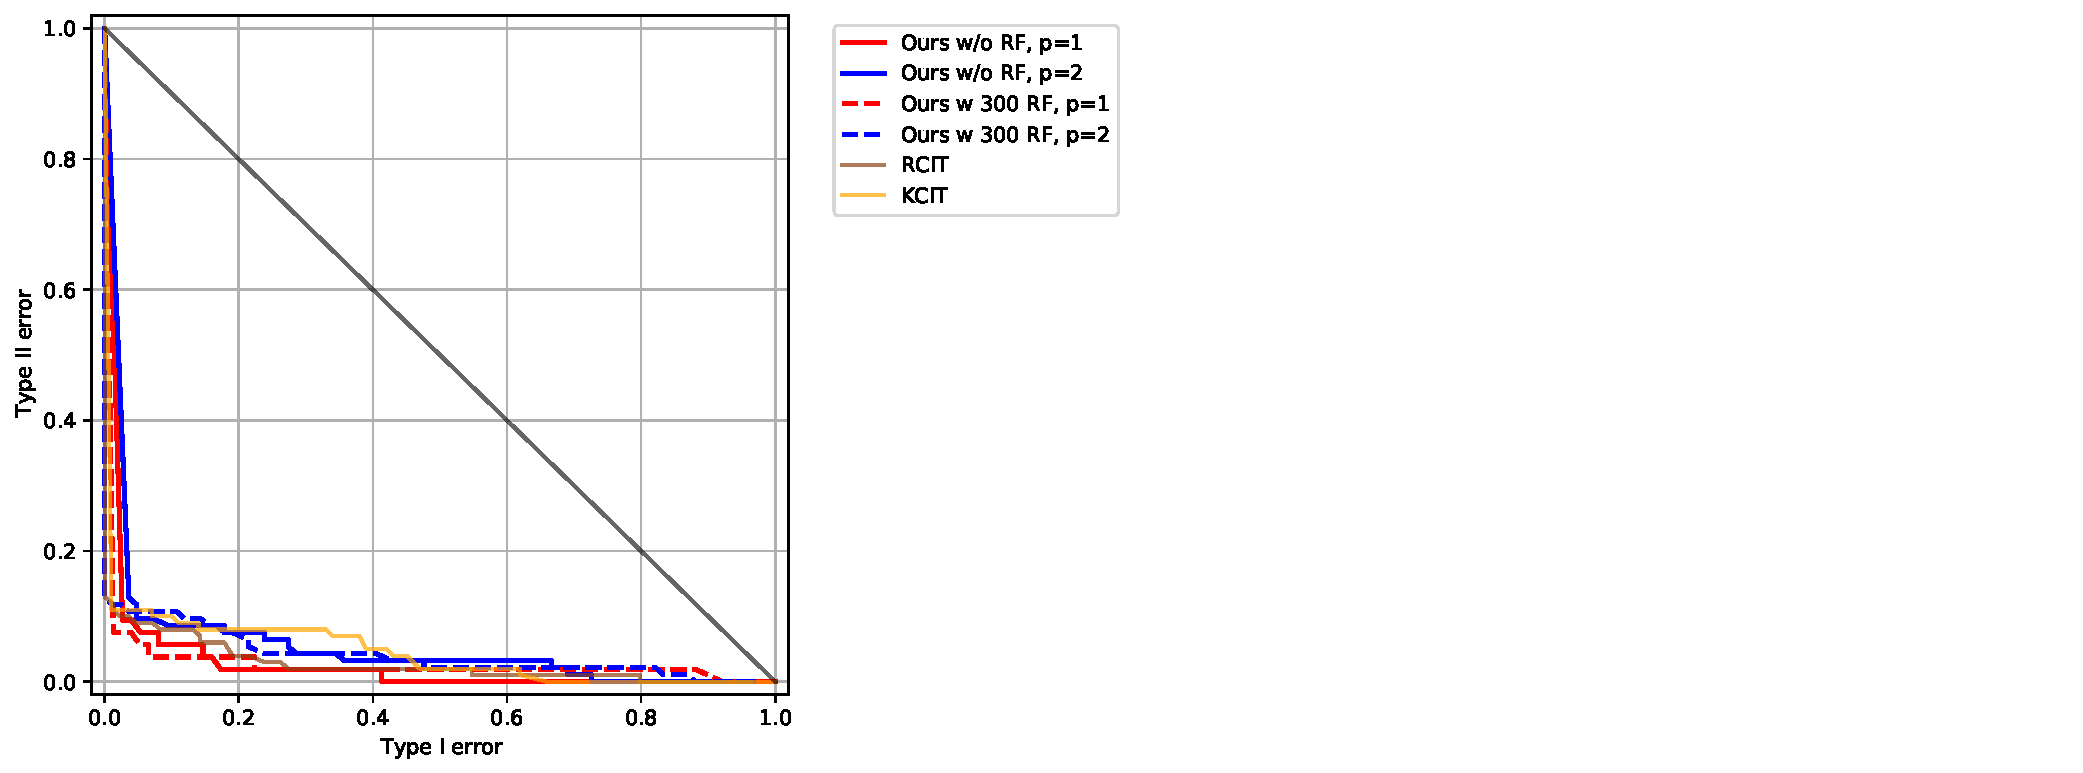
\includegraphics[width=0.85\textwidth]{figures/plots_v2_auc_2_False_gaussian_square.pdf}
%     \caption{Area under curve comparing our approaches (Section~\ref{sec:43}) with KCIT and RCIT on a $2$ dimensional problem, with $f(x)=x^2$. The number of samples is fixed at $600$, and the results are averaged over $100$ runs. We chose $J=3$, we did not optimize the positions of the $t_j$, neither the parameters of the gaussian kernels. We fixed the rank of the RLS estimation to $r=300$.}
%     \label{fig:auc2}
% \end{figure}


% \begin{figure*}
%     \centering
%     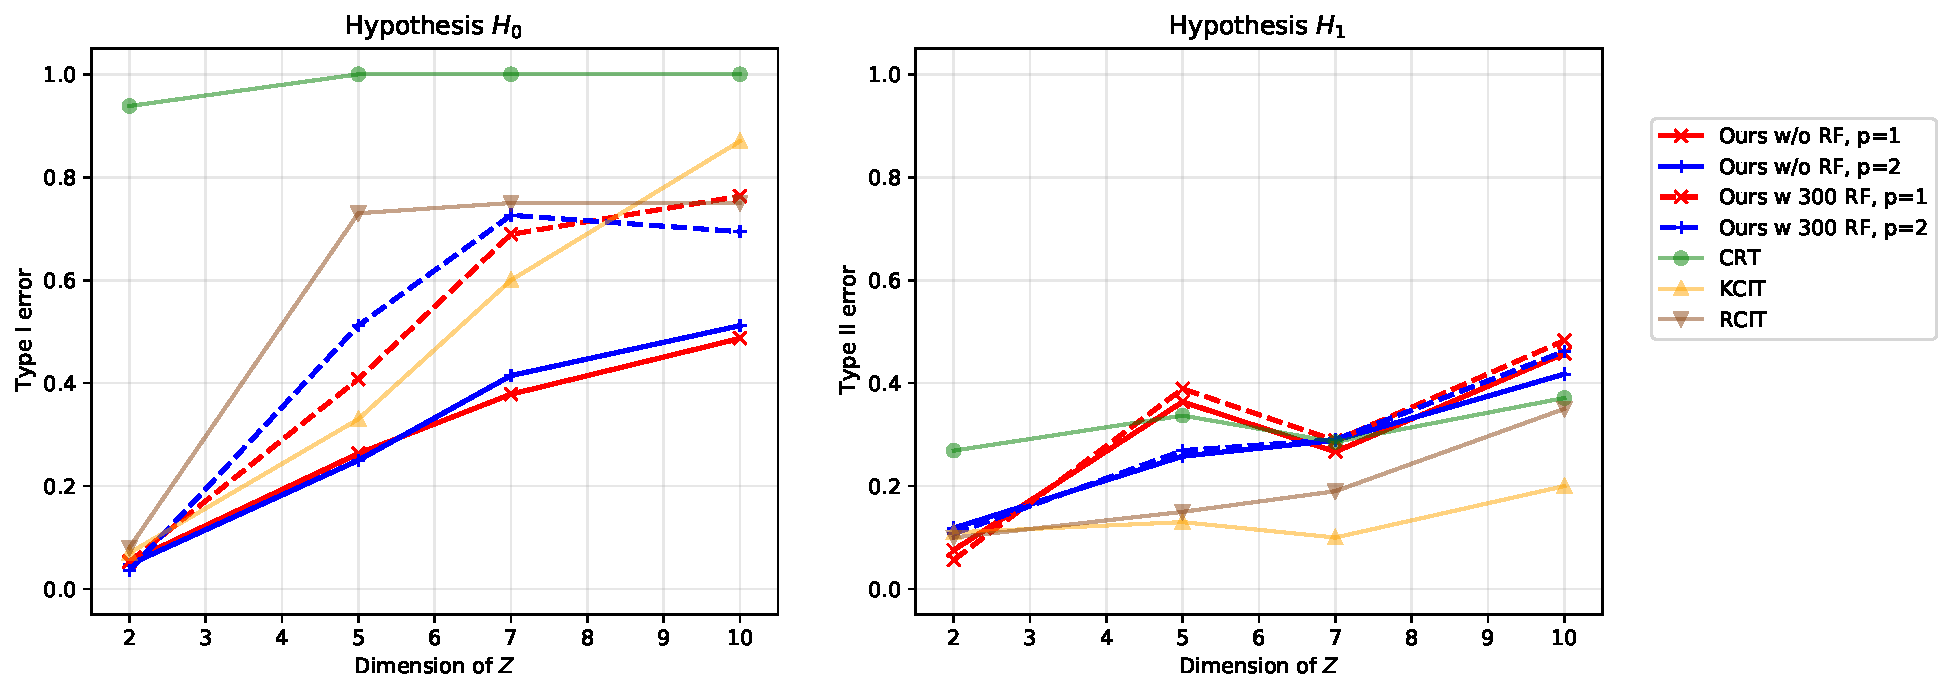
\includegraphics[width=0.9\textwidth]{figures/plots_v2_False_gaussian_square.pdf}
%     \caption{Comparison of our approach with RCIT, KCIT and CRT for various dimension of $Z$. On left, the problem is simulated from $H_0$ and we plotted the Type I error. On right from $H_1$ and we plotted the Type II error. The number of samples is fixed at $600$, and the results are averaged over $100$ runs. We chose $J=3$ , we did not optimize the positions of the $t_j$, neither the parameters of the gaussian kernels. We fixed the rank of the RLS estimation to $r=300$.}
%     \label{fig:type_error}
% \end{figure*}
\section{Conclusion}
We introduced a new kernel-based statistic for testing CI. We derived its asymptotic null distribution and designed a simple testing procedure that emerges from it. To our knowledge, we are the first article to propose an asymptotic test for CI with a tractable null distribution. Using various synthetic experiments, we demonstrated that our approach is competitive with other SoTA methods both in terms of type-I and type-II errors, even in the high dimensional setting.


% This work offers a new computationally efficient kernel-based test for conditional independence, supported by asymptotic theoretical guarantees. We show that comparing the $L^p$ distance between well chosen mean embeddings at a finite set of locations leads to a simple characterization of the conditional independence relation. Our method is flexible in the sense that the locations and the kernels used to embed the distributions can be chosen in order to maximize the power. 

% A first estimate of the metric can be obtained when one has access to observations from some specific conditional means. However, in practice, such samples are not available; we overcome this by estimating the unknown samples using regularized least-squares approximations of the conditional means. We obtain the asymptotic distribution of the resulting statistic and derive a consistent test from it. Furthermore, we reduce the computational complexity of the proposed method by considering random features expansions of kernels when fitting the regression models. We show that the choice of RLS estimators to estimate samples from the conditional means is valid in order to derive the asymptotic distribution of our statistic. However any generative method which allows to sample from the conditional means can be used to replace our RLS estimators: we leave this as an open question for further work.



% Our results on asymptotic distribution requires additional assumptions compared to the ones in~\cite{zhang2012kernel}. Indeed, we need conditions to ensure the convergence rate of the RLS estimator. However, in~\citep{zhang2012kernel}, the proof of their asymptotic law requires assumptions to ours to hold. In~\citep{strobl1702approximate}, to prove their asymptotic distribution, the authors assume to have access to samples from the conditional mean, which is in practice impossible. {\color{red}[sounds weird, check grammar.]} In our work, by adding Assumptions~\ref{ass:spectrum}-\ref{ass:source}, we show that the asymptotic law still holds with RLS estimate of the conditional expectation. 

% We proposed a new consistent test for conditional independence, for which we proved its asymptotic law. We compared it with several benchmark tests {\color{red}[sounds weird, need to improve the language also we need to see if we are indeed better and faster]}, showing our test is faster and more accurate than other methods. As further work, we plan to deploy our statistic in order to learn invariant representations {\color{red}[reference]}.
\section{Appendix: Proofs}
\subsection{On the Formulation of the Witness Function}
\label{form-witness}
Let $(\mathbf{t}_j)_{j=1}^J$ sampled independently from the $\Gamma$ distribution, then by definition of $d_{p,J}(\cdot,\cdot)$, we have that
\begin{align*}
\label{eq-dlp_J}
    d_{p,J}(P_{XZY},P_{\ddot{X}\otimes Y|Z}):=\left[\frac{1}{J}\sum_{j=1}^J \left|\mu_{P_{XZY},k_{\mathcal{\ddot{X}}}\cdot k_{\mathcal{Y}}}(\mathbf{t}_j)-\mu_{P_{\ddot{X}\otimes Y|Z},k_{\mathcal{\ddot{X}}}\cdot k_{\mathcal{Y}}}(\mathbf{t}_j)\right|^p\right]^{\frac{1}{p}},
\end{align*}
Moreover thanks to Assumption~\ref{assump-kernel}, we have that for any $(\mathbf{t}^{(1)},t^{(2)})\in\mathcal{\ddot{X}}\times\mathcal{Y}$ 
\begin{equation*}
    \mu_{P_{\ddot{X}\otimes Y|Z},k_{\mathcal{\ddot{X}}}\cdot k_{\mathcal{Y}}}(\mathbf{t}^{(1)},t^{(2)})=
    \mathbb{E}_{Z}\left[\mathbb{E}_{\ddot{X}}\left[k_{\mathcal{\ddot{X}}}(\mathbf{t}^{(1)},\ddot{X})|Z\right]
    \mathbb{E}_{Y}\left[k_{\mathcal{Y}}(t^{(2)},Y)|Z\right] \right]\; ,
\end{equation*}
and 
\begin{equation*}
    \mu_{P_{XZY},k_{\mathcal{\ddot{X}}}\cdot k_{\mathcal{Y}}}(\mathbf{t}^{(1)},t^{(2)})=
    \mathbb{E}\left[k_{\mathcal{\ddot{X}}}(\mathbf{t}^{(1)},\ddot{X})
 k_{\mathcal{Y}}(t^{(2)},Y) \right]\; .
\end{equation*}


Let us now introduce the following witness function
\begin{align*}
    \Delta(\mathbf{t}^{(1)},t^{(2)}) :=\mathbb{E}\left[\left(k_{\mathcal{\ddot{X}}}(\mathbf{t}^{(1)},\ddot{X})- \mathbb{E}_{\ddot{X}}\left[k_{\mathcal{\ddot{X}}}(\mathbf{t}^{(1)},\ddot{X})|Z\right]\right)\times\left(k_{\mathcal{Y}}(t^{(2)},Y)- \mathbb{E}_{Y}\left[k_{\mathcal{Y}}(t^{(2)},Y)|Z\right]\right)\right]\;.
\end{align*}
Therefore we obtain that

\begin{align*}
    \Delta(\mathbf{t}^{(1)},t^{(2)}) &=\mathbb{E}\left[k_{\mathcal{\ddot{X}}}(\mathbf{t}^{(1)},\ddot{X})(k_{\mathcal{Y}}(t^{(2)},Y)\right]\\ 
    &- \mathbb{E}\left[k_{\mathcal{\ddot{X}}}(\mathbf{t}^{(1)},\ddot{X})\mathbb{E}_{Y}\left[k_{\mathcal{Y}}(t^{(2)},Y)|Z\right]\right]\\
    &+ \mathbb{E}\left[\mathbb{E}_{\ddot{X}}\left[k_{\mathcal{\ddot{X}}}(\mathbf{t}^{(1)},\ddot{X})|Z\right] \mathbb{E}_{Y}\left[k_{\mathcal{Y}}(t^{(2)},Y)|Z\right] \right]\\
   &- \mathbb{E}\left[\mathbb{E}_{\ddot{X}}\left[k_{\mathcal{\ddot{X}}}(\mathbf{t}^{(1)},\ddot{X})|Z\right]k_{\mathcal{Y}}(t^{(2)},Y)\right]\;.
\end{align*}
Now remarks that
\begin{align*}
    \mathbb{E}\left[k_{\mathcal{\ddot{X}}}(\mathbf{t}^{(1)},\ddot{X})\mathbb{E}_{Y}\left[k_{\mathcal{Y}}(t^{(2)},Y)|Z\right]\right] &= \mathbb{E}\left[\mathbb{E}\left[k_{\mathcal{\ddot{X}}}(\mathbf{t}^{(1)},\ddot{X})\mathbb{E}_{Y}\left[k_{\mathcal{Y}}(t^{(2)},Y)|Z\right]\big|Z\right]\right]\\
    &=\mathbb{E}\left[\mathbb{E}_{Y}\left[k_{\mathcal{Y}}(t^{(2)},Y)|Z\right]  \mathbb{E}_{\ddot{X}}\left[k_{\mathcal{\ddot{X}}}(\mathbf{t}^{(1)},\ddot{X})|Z\right]\right]\;.
\end{align*}
Simiarly, we have that 
\begin{align*}
\mathbb{E}\left[\mathbb{E}_{\ddot{X}}\left[k_{\mathcal{\ddot{X}}}(\mathbf{t}^{(1)},\ddot{X})|Z\right]k_{\mathcal{Y}}(t^{(2)},Y)\right] = \mathbb{E}\left[\mathbb{E}_{Y}\left[k_{\mathcal{Y}}(t^{(2)},Y)|Z\right]  \mathbb{E}_{\ddot{X}}\left[k_{\mathcal{\ddot{X}}}(\mathbf{t}^{(1)},\ddot{X})|Z\right]\right]
\end{align*}
from which follows that 
\begin{align*}
    \Delta(\mathbf{t}^{(1)},t^{(2)}) & = \mathbb{E}\left[k_{\mathcal{\ddot{X}}}(\mathbf{t}^{(1)},\ddot{X})(k_{\mathcal{Y}}(t^{(2)},Y)\right] - \mathbb{E}\left[\mathbb{E}_{Y}\left[k_{\mathcal{Y}}(t^{(2)},Y)|Z\right]  \mathbb{E}_{\ddot{X}}\left[k_{\mathcal{\ddot{X}}}(\mathbf{t}^{(1)},\ddot{X})|Z\right]\right]\\
    &=  \mu_{P_{XZY},k_{\mathcal{\ddot{X}}}\cdot k_{\mathcal{Y}}}(\mathbf{t}^{(1)},t^{(2)}) - \mu_{P_{\ddot{X}\otimes Y|Z},k_{\mathcal{\ddot{X}}}\cdot k_{\mathcal{Y}}}(\mathbf{t}^{(1)},t^{(2)})\;.
\end{align*}


\subsection{Proof of Proposition~\lowercase{\ref{prop:rls-law}}}
\label{prv:rls-law}

\begin{proof} For all $j\in[J]$:
    
\begin{align}
  &\sqrt{n}\widetilde{\Delta}_{n,r}(\mathbf{t}^{(1)}_j,t^{(2)}_j)\\
  &= \sqrt{n}\frac{1}{n}\sum_{i=1}^n  \left(k_{\mathcal{\ddot{X}}}(\mathbf{t}^{(1)}_j,\ddot{x}_i)- h^{(1)}_{j,r}(z_i)\right)\left(k_{\mathcal{Y}}(t^{(2)}_j,y_i)- h^{(2)}_{j,r}(z_i)\right)\nonumber\\
  &= \sqrt{n}\Delta_{n}(\mathbf{t}^{(1)}_j,t^{(2)}_j)\label{eq:term-tcl}\\
  &+\sqrt{n} \frac1n\sum_{i=1}^n\left(k_{\mathcal{\ddot{X}}}(\mathbf{t}^{(1)}_j,\ddot{x}_i)-\mathbb{E}_{\ddot{X}}\left[k_{\mathcal{\ddot{X}}}(\mathbf{t}^{(1)}_j,\ddot{X})|Z=z_i\right]\right)\left(\mathbb{E}_{Y}\left[k_{\mathcal{Y}}(t^{(2)}_j,Y)|Z=z_i\right]- h^{(2)}_{j,r}(z_i)\right)\label{eq:term-cross1}\\
  &+\sqrt{n}\frac1n\sum_{i=1}^n\left(\mathbb{E}_{\ddot{X}}\left[k_{\mathcal{\ddot{X}}}(\mathbf{t}^{(1)}_j,\ddot{X})|Z=z_i\right]-h^{(1)}_{j,r}(z_i)\right)\left(k_{\mathcal{Y}}(t^{(2)}_j,y_i)-\mathbb{E}_{Y}\left[k_{\mathcal{Y}}(t^{(2)}_j,Y)|Z=z_i\right]\right)\label{eq:term-cross2}\\
  &+\sqrt{n}\frac1n\sum_{i=1}^n\left(\mathbb{E}_{\ddot{X}}\left[k_{\mathcal{\ddot{X}}}(\mathbf{t}^{(1)}_j,\ddot{X})|Z=z_i\right]-h^{(1)}_{j,r}(z_i)\right)\left(\mathbb{E}_{Y}\left[k_{\mathcal{Y}}(t^{(2)}_j,Y)|Z=z_i\right]-h^{(2)}_{j,r}(z_i)\right)\label{eq:term-cross3}
\end{align} 

Let us treat the four terms of this decomposition. The term~\eqref{eq:term-tcl} has been treated by Propostion~\ref{prop:oracle-law}, and satisfies, under the null hypothesis $H_0$
\begin{align*}
\sqrt{n}\Delta_{n}&(\mathbf{t}_j^{(1)},t_j^{(2)})\\
&\to_{n\to\infty} \mathcal{N}\left(0,\mathbb{E}\left[\left(k_{\mathcal{\ddot{X}}}(\mathbf{t}^{(1)}_j,\ddot{X})-\mathbb{E}_{\ddot{X}}\left[k_{\mathcal{\ddot{X}}}(\mathbf{t}^{(1)}_j,\ddot{X})|Z\right]\right)\left(k_{\mathcal{Y}}(t^{(2)}_j,Y)-\mathbb{E}_{Y}\left[k_{\mathcal{Y}}(t^{(2)}_j,Y)|Z\right]\right)\right]\right)
\end{align*}

Let us now show that the last term~\eqref{eq:term-cross3} converges towards $0$ in probability. Let us denote for all $j$, $e^{(1)}_{j}:z\to\mathbb{E}_{\ddot{X}}\left[k_{\mathcal{\ddot{X}}}(\mathbf{t}^{(1)}_j,\ddot{X})|Z=z\right] $ and $e^{(2)}_{j}:z\to\mathbb{E}_{Y}\left[k_{\mathcal{\ddot{X}}}(t^{(2)}_j,Y)|Z=z\right]$, both elements of $ H_{\mathcal{Z}}$ by Assumption~\ref{ass:source}. Then we have, for all $i\in[n]$:

\begin{align*}
   \left(e^{(1)}_{j}(z_i)-h^{(1)}_{j,r}(z_i)\right)\left(e^{(2)}_{j}(z_i)-h^{(2)}_{j,r}(z_i)\right)=\langle\left(e^{(1)}_{j}-h^{(1)}_{j,r}\right)\otimes\left(e^{(2)}_{j}-h^{(2)}_{j,r}\right), k_{\mathcal{Z}}(z_i,\cdot)\otimes k_{\mathcal{Z}}(z_i,\cdot)\rangle.
\end{align*}
Then we deduce, by denoting: $\mu_{ZZ} := \mathbb{E}\left[ k_{\mathcal{Z}}(Z,\cdot)k_{\mathcal{Z}}(Z,\cdot)\right]$ and $\hat{\mu}_{ZZ}:=\frac1n\sum_{i=1}^n k_{\mathcal{Z}}(z_i,\cdot)k_{\mathcal{Z}}(z_i,\cdot)$, that
\begin{align*}
    \frac1n\sum_{i=1}^n\left(\mathbb{E}_{\ddot{X}}\left[k_{\mathcal{\ddot{X}}}(\mathbf{t}^{(1)}_j,\ddot{X})|Z=z_i\right]-h^{(1)}_{j,r}(z_i)\right)\left(\mathbb{E}_{Y}\left[k_{\mathcal{Y}}(t^{(2)}_j,Y)|Z=z_i\right]-h^{(2)}_{j,r}(z_i)\right)\\
    = \langle\left(e^{(1)}_{j}-h^{(1)}_{j,r}\right)\otimes\left(e^{(2)}_{j}-h^{(2)}_{j,r}\right),\frac{1}{n}\sum_{i=1}^n k_{\mathcal{Z}}(z_i,\cdot)\otimes k_{\mathcal{Z}}(z_i,\cdot)\rangle\\
    =\langle\left(e^{(1)}_{j}-h^{(1)}_{j,r}\right)\otimes\left(e^{(2)}_{j}-h^{(2)}_{j,r}\right),\mu_{ZZ}\rangle+\langle\left(e^{(1)}_{j}-h^{(1)}_{j,r}\right)\otimes\left(e^{(2)}_{j}-h^{(2)}_{j,r}\right),\hat{\mu}_{ZZ}-\mu_{ZZ}\rangle\;.
\end{align*}
Then remarks that:
\begin{align*}
    \lvert\langle\left(e^{(1)}_{j}-h^{(1)}_{j,r}\right)\otimes\left(e^{(2)}_{j}-h^{(2)}_{j,r}\right),\mu_{ZZ}\rangle\rvert&=\lvert\mathbb{E}_Z\left[\left(e^{(1)}_{j}(Z)-h^{(1)}_{j,r}(Z)\right)\left(e^{(2)}_{j}(Z)-h^{(2)}_{j,r}(Z)\right)\right]\rvert\\
    &\leq \lVert e^{(1)}_{j}-h^{(1)}_{j,r}\rVert_{L^2(P_Z)} \lVert  e^{(2)}_{j}-h^{(2)}_{j,r}\rVert_{L^2(P_Z)} 
\end{align*}
Under the Assumptions~\ref{ass:spectrum}-\ref{ass:source}, for $\lambda_{r} = \frac{1}{r^{\beta+\gamma}}$, we have, using the results from~\cite{fischer2020sobolev}: $\lVert  e^{(1)}_{j}-h^{(1)}_{j,r}\rVert_{L^2(P_Z)}^2\leq \frac{C\tau^2}{r^{\frac{\beta}{\beta+\gamma}}}$ with probability $1-4e^{-\tau}$ and  $ \lVert e^{(2)}_{j}-h^{(2)}_{j,r}\rVert_{L^2(P_Z)}^2 \leq \frac{C\tau^2}{r^{\frac{\beta}{\beta+\gamma}}}$ with probability $1-4e^{-\tau}$, for some constant $C$ independent from $n$ and $\tau$. then by union bound, we deduce with probability $1-8e^{-\tau}$ we have:
\begin{align*}
    \sqrt{n}\lvert\langle\left(e^{(1)}_{j}-h^{(1)}_{j,r}\right)\otimes\left(e^{(2)}_{j}-h^{(2)}_{j,r}\right),\mu_{ZZ}\rangle\rvert\leq \sqrt{n}\frac{C^2\tau^4}{r^{\frac{\beta}{\beta+\gamma}}}
\end{align*}

Then, if $\sqrt{n}\in o(r^{\frac{\beta}{\beta+\gamma}})$, we have:
$ \sqrt{n}\lvert\langle\left(e^{(1)}_{j}-h^{(1)}_{j,r}\right)\otimes\left(e^{(2)}_{j}-h^{(2)}_{j,r}\right),\mu_{ZZ}\rangle\rvert\to 0$ in probability when $n\to\infty$. Moreover:
\begin{align*}
    \lvert \left(e^{(1)}_{j}-h^{(1)}_{j,r}\right)\otimes\left(e^{(2)}_{j}-h^{(2)}_{j,r}\right),\hat{\mu}_{ZZ}-\mu_{ZZ}\rangle\rvert\leq \lVert e^{(1)}_{j}-h^{(1)}_{j,r}\rVert_{ H_\mathcal{Z}} \lVert e^{(2)}_{j}-h^{(2)}_{j,r}\rVert_{ H_\mathcal{Z}}\lVert\hat{\mu}_{ZZ}-\mu_{ZZ}\rVert_{ H_\mathcal{Z}\otimes H_\mathcal{Z}}\; ,
\end{align*}
and by Markov inequality, $\lVert\hat{\mu}_{ZZ}-\mu_{ZZ}\rVert_{H_\mathcal{Z}\otimes H_\mathcal{Z}} \leq \sqrt{\frac{C'}{n\delta}}$ with probability $1-\delta$ for some constant $C'$. Moreover, under Assumption~\ref{ass:spectrum}-\ref{ass:source}, we have $\lVert e^{(1)}_{j}-h^{(1)}_{j,r}\rVert_{ H_\mathcal{Z}}\to 0$ and $\lVert e^{(2)}_{j}-h^{(2)}_{j,r}\rVert_{ H_\mathcal{Z}}\to 0$ in probability. Then, we deduce that $\sqrt{n}\lvert \langle\left(e^{(1)}_{j}-h^{(1)}_{j,r}\right)\otimes\left(e^{(2)}_{j}-h^{(2)}_{j,r}\right),\hat{\mu}_{ZZ}-\mu_{ZZ}\rangle\rvert\to 0$ in probability. Finally, the term~\eqref{eq:term-cross3} goes to $0$ in probability. 



The terms~\eqref{eq:term-cross1} and~\eqref{eq:term-cross2} are similar and can be treated the same way. We only focus on the term~\eqref{eq:term-cross1}. For all $i\in[n]$:
\begin{align*}
\lvert\frac1n\sum_{i=1}^n\left(k_{\mathcal{\ddot{X}}}(\mathbf{t}^{(1)}_j,\ddot{x}_i)-\mathbb{E}_{\ddot{X}}\left[k_{\mathcal{\ddot{X}}}(\mathbf{t}^{(1)}_j,\ddot{X})|Z=z_i\right]\right)\left(\mathbb{E}_{Y}\left[k_{\mathcal{Y}}(t^{(2)}_j,Y)|Z=z_i\right]- h^{(2)}_{j,r}(z_i)\right)\rvert\\
  =\lvert\frac1n\sum_{i=1}^n\langle k_{\mathcal{\ddot{X}}}(t^{(1)}_j,\cdot),k_{\mathcal{\ddot{X}}}(\ddot{x}_i,\cdot)-\mathbb{E}_{\ddot{X}}\left[k_{\mathcal{\ddot{X}}}(\ddot{X},\cdot)|Z=z_i\right]\rangle_{ H_\mathcal{\ddot{X}}}
  \langle e^{(2)}_{j}-h^{(2)}_{j,r},k_{\mathcal{Z}}(z_i,\cdot)\rangle_{ H_\mathcal{Z}}\rvert\\
  =\lvert\frac1n\sum_{i=1}^n\langle k_{\mathcal{\ddot{X}}}(t^{(1)},\cdot)\otimes \left(e^{(2)}_{j}-h^{(2)}_{j,r}\right),\left(k_{\mathcal{\ddot{X}}}(\ddot{x}_i,\cdot)-\mathbb{E}_{\ddot{X}}\left[k_{\mathcal{\ddot{X}}}(\ddot{X},\cdot)|Z=z_i\right]\right)\otimes k_{\mathcal{Z}}(z_i,\cdot)\rangle_{ H_\mathcal{\ddot{X}}\otimes H_\mathcal{Z}}\rvert\\
  =\lvert\langle k_{\mathcal{\ddot{X}}}(t^{(1)},\cdot)\otimes \left(e^{(2)}_{j}-h^{(2)}_{j,r}\right),\frac1n\sum_{i=1}^n\left(k_{\mathcal{\ddot{X}}}(\ddot{x}_i,\cdot)-\mathbb{E}_{\ddot{X}}\left[k_{\mathcal{\ddot{X}}}(\ddot{X},\cdot)|Z=z_i\right]\right)\otimes k_{\mathcal{Z}}(z_i,\cdot)\rangle_{ H_\mathcal{\ddot{X}}\otimes H_\mathcal{Z}}\rvert\\
  \leq \lVert k_{\mathcal{\ddot{X}}}(t^{(1)},\cdot)\rVert_{ H_\mathcal{\ddot{X}}}\lVert e^{(2)}_{j}-h^{(2)}_{j,r}\rVert_{H_\mathcal{Z}}\left(\lVert \hat{\mu}^1_{\ddot{X}Z}-\mu_{\ddot{X}Z}\rVert_{ H_\mathcal{\ddot{X}}\otimes H_\mathcal{Z}}+ \lVert\hat{\mu}^2_{\ddot{X}}-\mu_{\ddot{X}Z}\rVert_{ H_\mathcal{\ddot{X}}\otimes H_\mathcal{Z}}\right)
\end{align*}
where: $\hat{\mu}^1_{\ddot{X}Z} := \frac1n\sum_{i=1}^nk_{\mathcal{\ddot{X}}}(\ddot{x}_i,\cdot)\otimes k_{\mathcal{Z}}(z_i,\cdot)$, $\hat{\mu}^2_{\ddot{X}Z}:=\frac1n\sum_{i=1}^n\mathbb{E}_{\ddot{X}}\left[k_{\mathcal{\ddot{X}}}(\ddot{X},\cdot)|Z=z_i\right]\otimes k_{\mathcal{Z}}(z_i,\cdot)$, and $\mu_{\ddot{X}Z}:=\mathbb{E}\left[k_{\mathcal{Y}}(y,\cdot)k_{\mathcal{Z}}(z,\cdot)\right]$.

By the law of large numbers, we have: $\hat{\mu}^1_{\ddot{X}Z}$ and $\hat{\mu}^2_{\ddot{X}Z}$ converge almost surely towards $\mu_{\ddot{X}Z}$. Moreover by Markov inequality, $\lVert\hat{\mu}^1_{\ddot{X}Z}-\mu_{\ddot{X}Z}\rVert_{ H_\mathcal{\ddot{X}}\otimes H_\mathcal{Z}} \leq \sqrt{\frac{C}{n\delta}}$ with probability $1-\delta$, and  $\lVert\hat{\mu}^2_{\ddot{X}Z}-\mu_{\ddot{X}Z}\rVert_{ H_\mathcal{\ddot{X}}\otimes H_\mathcal{Z}} \leq \sqrt{\frac{C}{n\delta}}$ with probability $1-\delta$. Then with probability $1-2\delta$, $\sqrt{n}\left(\lVert\hat{\mu}^1_{\ddot{X}Z}-\mu_{\ddot{X}Z}\rVert_{ H_\mathcal{\ddot{X}}\otimes H_\mathcal{Z}}+\lVert\hat{\mu}^2_{\ddot{X}Z}-\mu_{\ddot{X}Z}\rVert_{ H_\mathcal{\ddot{X}}\otimes H_\mathcal{Z}} \right)\leq2\sqrt{\frac{C}{\delta}}$. Moreover, under Assumption~\ref{ass:spectrum}-\ref{ass:source}, using the results from~\cite{fischer2020sobolev}, we have that $\lVert e^{(2)}_{j}-h^{(2)}_{j,r}\rVert_{H_\mathcal{Z}}$ converges towards $0$ in probability. Then the term~\eqref{eq:term-cross1}
converges in probability towards $0$. The same reasoning holds for~\eqref{eq:term-cross2}. 

Finally, by Slutsky's Lemma:
\begin{align*}
    \sqrt{n}\widetilde{\Delta}_{n,r}&(\mathbf{t}^{(1)}_j,t^{(2)}_j)\\
    &\to_{n\to\infty} \mathcal{N}\left(0,\mathbb{E}\left[\left(k_{\mathcal{\ddot{X}}}(\mathbf{t}^{(1)}_j,\ddot{X})-\mathbb{E}_{\ddot{X}}\left[k_{\mathcal{\ddot{X}}}(\mathbf{t}^{(1)}_j,\ddot{X})|Z\right]\right)\left(k_{\mathcal{Y}}(t^{(2)}_j,Y)-\mathbb{E}_{Y}\left[k_{\mathcal{Y}}(t^{(2)}_j,Y)|Z\right]\right)\right]\right).
\end{align*}
Now we have:
\begin{align*}
    \widetilde{\mathbf{S}}_{n,r}=\left(\widetilde{\Delta}_{n,r}(\mathbf{t}^{(1)}_j,t^{(2)}_j)\right)_{j\in[J]}=\left(\Delta_{n}(\mathbf{t}^{(1)}_j,t^{(2)}_j)\right)_{j\in[J]}+ \left(\widetilde{\Delta}_{n,r}(\mathbf{t}^{(1)}_j,t^{(2)}_j)-\Delta_{n}(\mathbf{t}^{(1)}_j,t^{(2)}_j)\right)_{j\in[J]}
\end{align*}
 and  we have shown that $\sqrt{n}\left(\widetilde{\Delta}_{n,r_n}(\mathbf{t}^{(1)}_j,t^{(2)}_j)-\Delta_{n}(\mathbf{t}^{(1)}_j,t^{(2)}_j)\right)_{j\in[J]}$ goes to $0$ in probability. Then by Slutsky Lemma and Proposition~\ref{prop:oracle-law}, we get: $\widetilde{\mathbf{S}}_{n,r_n}\to\mathcal{N}\left(0,\bm{\Sigma}\right)$.%, under $H_0$ we have:
% \begin{align*}
%     \left(\mu_{\text{w},r}(\mathbf{t}^{(1)}_j,t^{(2)}_j)\right)_{j\in[J]}\to \mathcal{N}\left(0,\Sigma_J\right).
% \end{align*}
%with $\Sigma_J=\left(\mathbb{E}\left[\left(k_{\mathcal{\ddot{X}}}(\mathbf{t}_i^{(1)},\ddot{X})-\mathbb{E}_{\ddot{X}}\left[k_{\mathcal{\ddot{X}}}(\mathbf{t}_i^{(1)},\ddot{X})|Z\right]\right)\left(k_{\mathcal{Y}}(t_j^{(2)},Y)-\mathbb{E}_{Y}\left[k_{\mathcal{Y}}(t_j^{(2)},Y)|Z\right]\right)\right]\right)_{i,j\in[J]}$. Then by Slutsky Lemma, we get: $\hat{V}_n\to\mathcal{N}\left(0,\Sigma_J\right)$.

Let $r>0$. Under $H_1$, $\mathbf{\mathbf{S}}_{n,r_n}\to \mathbf{S}\neq 0$. Let consider a realization of $(\mathbf{t}^{(1)}_j,t_j^{(2)})_{j\in[J]}$ such that $\lVert \mathbf{S}\rVert_p\neq 0$. So $P(n^{p/2}\lVert \mathbf{S}_{n,r_n}\rVert_p\geq r)\to 1$ as $n\to\infty$ because $\lVert \mathbf{S}\rVert_p\neq 0$.
\end{proof}
\newpage
\subsection{Proof of Proposition~\lowercase{\ref{prop:norm-law}}}
\label{prv:norm-law}
\begin{proof}
First notice that:
\begin{align*}
  \bm{\widetilde{\Sigma}}_{n,r}&:=\frac{1}{n}\sum_{i=1}^n \widetilde{\mathbf{u}}_{i,r}\widetilde{\mathbf{u}}_{i,r}^T+\delta_n \text{Id}_J  \\
  &=  \bm{\widehat{\Sigma}}_{n}+\frac1n\sum_{i=1}^n \widehat{\mathbf{u}}_{i}\left(\widetilde{\mathbf{u}}_{i,r}-\widehat{\mathbf{u}}_{r}\right)^T+\frac1n\sum_{i=1}^n \left(\widetilde{\mathbf{u}}_{i,r}-\widehat{\mathbf{u}}_{r}\right)\widehat{\mathbf{u}}_{i}^T\\
  &+\frac1n\sum_{i=1}^n\left(\widetilde{\mathbf{u}}_{i,r}-\widehat{\mathbf{u}}_{r}\right) \left(\widetilde{\mathbf{u}}_{i,r}-\widehat{\mathbf{u}}_{r}\right)^T+\delta_n \text{Id}_J
\end{align*}

By the law of large numbers, we get that under $H_0$: $\bm{\widehat{\Sigma}}_{n}\to\bm{\Sigma}$. Moreover:
\begin{align*}
    \left[\frac1n\sum_{i=1}^n \widehat{\mathbf{u}}_{i}\left(\widetilde{\mathbf{u}}_{i,r}-\widehat{\mathbf{u}}_{r}\right)^T\right]_{kl} = \frac{1}{n}\sum_{i=1}^n\left(k_{\mathcal{Y}}(t_k^{(2)},y_i)-\mathbb{E}_{Y}\left[k_{\mathcal{Y}}(t_k^{(2)},Y)|Z=z_i\right]\right)\left(\mathbb{E}_{\ddot{X}}\left[k_{\mathcal{\ddot{X}}}(\mathbf{t}_l^{(1)},\ddot{X})|Z=z_i\right]-h^{(1)}_{l,r}(z_i)\right)
\end{align*}
which has been proven to converge in probability to $0$ in the proof of Proposition~\ref{prop:rls-law}. Then $\frac1n\sum_{i=1}^n \widehat{\mathbf{u}}_{i}\left(\widetilde{\mathbf{u}}_{i,r}-\widehat{\mathbf{u}}_{r}\right)^T$ converges in probability to $0$. Similarly $\frac1n\sum_{i=1}^n \left(\widetilde{\mathbf{u}}_{i,r}-\widehat{\mathbf{u}}_{r}\right)\widehat{\mathbf{u}}_{i}^T$ and  $\frac1n\sum_{i=1}^n\left(\widetilde{\mathbf{u}}_{i,r}-\widehat{\mathbf{u}}_{r}\right) \left(\widetilde{\mathbf{u}}_{i,r}-\widehat{\mathbf{u}}_{r}\right)^T$ also converge in probability to $0$. Then by Slutsky Lemma, $ \bm{\widetilde{\Sigma}}_{n,r}$ converges in probability to $\bm{\Sigma}$. By Slutsky's lemma (again) and by Propostion~\ref{prop:rls-law}, we have that:
$\bm{\widetilde{\Sigma}}_{n,r}^{-1}\bm{\widetilde{S}}_{n,r}$ converges to a standard gaussian distribution $\mathcal{N}(0,\text{Id})$. The second part of the proposition is the same than the proof of Proposition~\ref{prop:rls-law}.
\end{proof}
% Let denote the operator $R:\ddot{\mathcal{X}}\rightarrow\mathcal{Z}$ defined as:
% $R =\left(\Sigma^{k_\mathcal{Z},k_\mathcal{Z}}_{p_{ZZ}}\right)^{-1}\Sigma^{k_\mathcal{Z},k_{\ddot{\mathcal{X}}}}_{p_{Z\ddot{X}}}$. 
% Let denote $R_M$ defined using the approximated random features kernel spaces: $R_M =\left(\Sigma^{k_{\mathcal{Z},M},k_{\mathcal{Z},M}}_{p_{ZZ}}\right)^{-1}\Sigma^{k_{\mathcal{Z},M},k_{\ddot{\mathcal{X}},M}}_{p_{Z\ddot{X}}}$
% Let show that: for all $u,v$
% \begin{align*}
%     \langle R_M k_{\ddot{\mathcal{X}},M}(u,\cdot),k_{\mathcal{Z},M}(v,\cdot)\rangle_{ H_{\mathcal{Z},M}}\to_{M\to\infty}     \langle R k_{\ddot{\mathcal{X}}}(u,\cdot),k_{\mathcal{Z}}(v,\cdot)\rangle_{ H_\mathcal{Z}}\text{ in probability} 
% \end{align*}

% We have:
% \begin{align*}
%     \langle R k_{\ddot{\mathcal{X}}}(u,\cdot),k_{\mathcal{Z}}(v,\cdot)\rangle_{ H_{\mathcal{Z}}} =     \langle \left(\Sigma^{k_\mathcal{Z},k_\mathcal{Z}}_{p_{ZZ}}\right)^{-1/2}R k_{\ddot{\mathcal{X}}}(u,\cdot),\left(\Sigma^{k_\mathcal{Z},k_\mathcal{Z}}_{p_{ZZ}}\right)^{-1/2}k_{\mathcal{Z}}(v,\cdot)\rangle_{L^2(p_Z)}
% \end{align*}

% \begin{align*}
%     \langle R_M k_{\ddot{\mathcal{X}},M}(u,\cdot),k_{\mathcal{Z},M}(v,\cdot)\rangle_{ H_{\mathcal{Z},M}} =     \langle \left(\Sigma^{k_{\mathcal{Z},M},k_{\mathcal{Z},M}}_{p_{ZZ}}\right)^{-1/2}R_M k_{\ddot{\mathcal{X}},M}(u,\cdot),\left(\Sigma^{k_{\mathcal{Z},M},k_{\mathcal{Z},M}}_{p_{ZZ}}\right)^{-1/2}k_{\mathcal{Z},M}(v,\cdot)\rangle_{L^2(p_Z)} 
% \end{align*}

% One can notice that

% \begin{align*}
%     \Sigma^{k_{\mathcal{Z},M},k_{\mathcal{Z},M}}_{p_{ZZ}} = \frac1M \sum_{i=1}^M \xi_i
% \end{align*}
% where $\xi_i = \phi_{\theta_i}\otimes\phi_{\theta_i}$ are i.i.d. copies. And $\Sigma^{k_{\mathcal{Z},M},k_{\mathcal{Z},M}}_{p_{ZZ}} = \mathbb{E}(\xi_1)$. Then:
% \begin{align*}
%     \mathbb{P}\left[\lVert\Sigma^{k_{\mathcal{Z},M},k_{\mathcal{Z},M}}_{p_{ZZ}}- \Sigma^{k_{\mathcal{Z}},k_{\mathcal{Z}}}_{p_{ZZ}}\rVert_{HS(L^2(p_Z),L^2(p_Z))} \geq \epsilon\right]&\leq  \frac{\mathbb{E}\left[\lVert\Sigma^{k_{\mathcal{Z},M},k_{\mathcal{Z},M}}_{p_{ZZ}}- \Sigma^{k_{\mathcal{Z}},k_{\mathcal{Z}}}_{p_{ZZ}}\rVert_{HS(L^2(p_Z),L^2(p_Z))}^2 \right]}{\epsilon^2}\\
%     &\leq \frac{1}{M\epsilon}\mathbb{E}\left[\lVert \xi_1-\mathbb{E}(x_1)\rVert_{HS(L^2(p_Z),L^2(p_Z))}\right]
% \end{align*}
% Then we deduce:
% \begin{align*}
% \lVert\Sigma^{k_{\mathcal{Z},M},k_{\mathcal{Z},M}}_{p_{ZZ}}- \Sigma^{k_{\mathcal{Z}},k_{\mathcal{Z}}}_{p_{ZZ}}\rVert_{HS(L^2(p_Z),L^2(p_Z))} \to 0 \text{ in probability.}
% \end{align*}

% \begin{align*}
% \lVert\Sigma^{k_{\mathcal{Z},M},k_{\ddot{\mathcal{X}},M}}_{p_{Z\ddot{X}}}- \Sigma^{k_{\mathcal{Z}},k_{\ddot{\mathcal{X}}}}_{p_{Z\ddot{X}}}\rVert_{HS(L^2(p_{\ddot{X}}),L^2(p_Z))} \to 0 \text{ in probability.}
% \end{align*}

% Then one can show that:

% \begin{align*}
% \lVert\left(\Sigma^{k_{\mathcal{Z},M},k_{\mathcal{Z},M}}_{p_{ZZ}}\right)^{-1/2}- \left(\Sigma^{k_{\mathcal{Z}},k_{\mathcal{Z}}}_{p_{ZZ}}\right)^{-1/2} \rVert_{HS(L^2(p_Z),L^2(p_Z))}\to 0 \text{ in probability.}
% \end{align*}

% \begin{align*}
% \lVert \left(\Sigma^{k_{\mathcal{Z},M},k_{\mathcal{Z},M}}_{p_{ZZ}}\right)^{-1/2}R_M- \left(\Sigma^{k_{\mathcal{Z}},k_{\mathcal{Z}}}_{p_{ZZ}}\right)^{-1/2} R\rVert_{HS(L^2(p_{\ddot{X}}),L^2(p_Z))} \to 0 \text{ in probability.}
% \end{align*}
% Moreover since $k_{\ddot{\mathcal{X}},M}$ converges uniformly in probability towards $k_{\ddot{\mathcal{X}}}$ on the compact $\ddot{\mathcal{X}}$. The same argument holds for $k_{\mathcal{Z},M}$. Then:
% \begin{align*}
%     \lVert k_{\ddot{\mathcal{X}},M}(v,\cdot)-k_{\ddot{\mathcal{X}}}(v,\cdot)\rVert_{L^2(p_{\ddot{\mathcal{X}}})}\to 0\text{ in probability}
% \end{align*}
% \begin{align*}
%     \lVert k_{\mathcal{Z}}(u,\cdot)-k_{\mathcal{Z}}(u,\cdot)\rVert_{L^2(p_{\mathcal{Z}})}\to 0\text{ in probability}
% \end{align*}
% Then:

% \begin{align*}
%   \lvert \langle R_M k_{\ddot{\mathcal{X}},M}(u,\cdot),k_{\mathcal{Z},M}(v,\cdot)\rangle_{ H_{\mathcal{Z},M}}-    \langle R k_{\ddot{\mathcal{X}}}(u,\cdot),k_{\ddot{\mathcal{X}}}(v,\cdot)\rangle_{ H_\mathcal{Z}}\rvert\\
%   \leq \lVert \left(\Sigma^{k_{\mathcal{Z},M},k_{\mathcal{Z},M}}_{p_{ZZ}}\right)^{-1/2}R_M- \left(\Sigma^{k_{\mathcal{Z}},k_{\mathcal{Z}}}_{p_{ZZ}}\right)^{-1/2} R\rVert_{HS(L^2(p_{\ddot{X}}),L^2(p_Z))} \lVert k_{\ddot{\mathcal{X}},M}(u,\cdot)\rVert_{L^2(p_{\ddot{X}})} \lVert k_{\mathcal{Z},M}(v,\cdot)\rVert_{L^2(p_{Z})} \lVert\left(\Sigma^{k_{\mathcal{Z},M},k_{\mathcal{Z},M}}_{p_{ZZ}}\right)^{-1/2}\rVert_{HS(L^2(p_{Z}),L^2(p_Z))} \\
%   +\lVert\left(\Sigma^{k_{\mathcal{Z},M},k_{\mathcal{Z},M}}_{p_{ZZ}}\right)^{-1/2}- \left(\Sigma^{k_{\mathcal{Z}},k_{\mathcal{Z}}}_{p_{ZZ}}\right)^{-1/2} \rVert_{HS(L^2(p_{Z}),L^2(p_Z))}\lVert k_{\ddot{\mathcal{X}},M}(u,\cdot)\rVert_{L^2(p_{\ddot{X}})} \lVert k_{\mathcal{Z},M}(v,\cdot)\rVert_{L^2(p_{Z})} \lVert\left(\Sigma^{k_{\mathcal{Z}},k_{\mathcal{Z}}}_{p_{ZZ}}\right)^{-1/2} R\rVert_{HS(L^2(p_{\ddot{X}}),L^2(p_Z))} \\
%   +\lVert k_{\ddot{\mathcal{X}},M}(u,\cdot)- k_{\ddot{\mathcal{X}}}(u,\cdot)\rVert_{L^2(p_{\ddot{X}})}\lVert\left(\Sigma^{k_{\mathcal{Z}},k_{\mathcal{Z}}}_{p_{ZZ}}\right)^{-1/2} \rVert_{HS(L^2(p_{Z}),L^2(p_Z))}\lVert k_{\mathcal{Z},M}(v,\cdot)\rVert_{L^2(p_Z)} \lVert\left(\Sigma^{k_{\mathcal{Z}},k_{\mathcal{Z}}}_{p_{ZZ}}\right)^{-1/2} R\rVert_{HS(L^2(p_{\ddot{X}}),L^2(p_Z))}\\
%   +\lVert k_{\mathcal{Z},M}(v,\cdot)- k_{\mathcal{Z}}(v,\cdot)\rVert_{L^2(p_{Z})}\lVert\left(\Sigma^{k_{\mathcal{Z}},k_{\mathcal{Z}}}_{p_{ZZ}}\right)^{-1/2} \rVert_{HS(L^2(p_{Z}),L^2(p_Z))} \lVert k_{\ddot{\mathcal{X}}}(u,\cdot)\rVert_{L^2(p_{\ddot{X}})} \lVert\left(\Sigma^{k_{\mathcal{Z}},k_{\mathcal{Z}}}_{p_{ZZ}}\right)^{-1/2} R\rVert_{HS(L^2(p_{\ddot{X}}),L^2(p_Z))}
% \end{align*}

% Finally we have shown that for all $u,v$:
% \begin{align*}
%     \langle R_M k_{\ddot{\mathcal{X}},M}(u,\cdot),k_{\mathcal{Z},M}(v,\cdot)\rangle_{ H_{\mathcal{Z},M}}\to_{M\to\infty}     \langle R k_{\ddot{\mathcal{X}}}(u,\cdot),k_{\mathcal{Z}}(v,\cdot)\rangle_{ H_\mathcal{Z}}\text{ in probability} 
% \end{align*}

% \section{A note on finding }
% \label{sec-theoritical-findings}

\section{Appendix: Additional Experiments}
\subsection{A note on the computation of Oracle statistic in Figure~\ref{fig-illustation-theory}}
\label{sec-theoritical-findings}

To compute the oracle statistic we needed to compute exactly the conditional expectation implied in our statistic. In the case of gaussian kernels and gaussian distributed data for $Z$, the computation of this conditional expectation is reduced to the computation of moment-generating function of a non-centered $\chi^2$ distribution.

\newpage
\subsection{Choice of the rank regression $r$}
\label{sec-rank-rn}
In this experiment, we show the effect of the rank regression $r$ on the performances of our proposed method. For that purpose, in Figure~\ref{fig-rn-dependence}, we consider the two problems presented in~\eqref{exp-strobl-h0} and~\eqref{exp-strobl-h1}  with Gaussian noises and show the type-I and type-II when varying the ratio $r/n$ for multiple sample size $n$. We observe that the rank $r$ does not affect the power of the method, however we observe that the type-I error decreases as the ratio increases. Therefore the rank $r$ allows in practice to deal with the tradeoff between the computational time and the control of the type-I error.

\begin{figure*}[ht]
\begin{tabular}{cccc} 
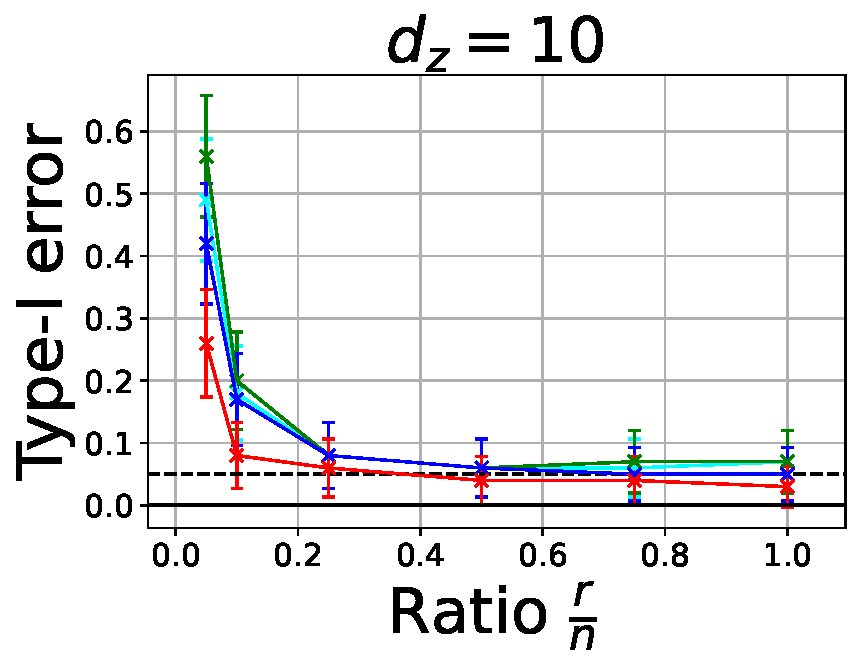
\includegraphics[height=3cm]{sections/appendix/independence_testing_kernel/figures_r_n/fig_ours_r_n_typeI.pdf}& 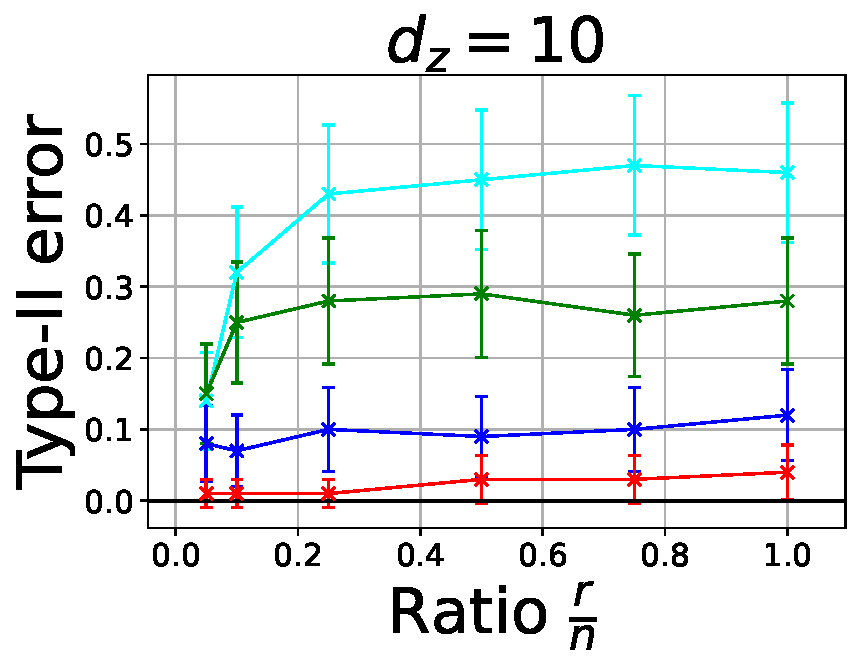
\includegraphics[height=3cm]{sections/appendix/independence_testing_kernel/figures_r_n/fig_ours_r_n_typeII.pdf}&
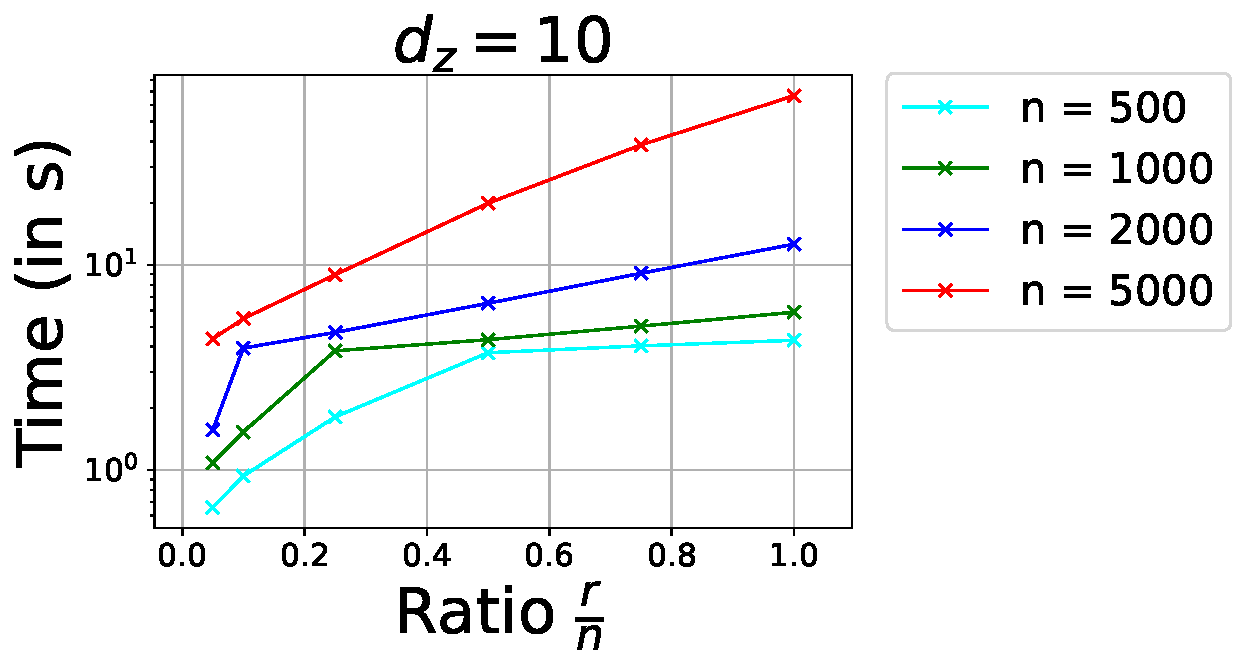
\includegraphics[height=3cm]{sections/appendix/independence_testing_kernel/figures_r_n/fig_ours_r_n_time.pdf}\\
\end{tabular}
\caption{Comparison of the type-I error at level $\alpha=0.05$ (dashed line) and the type-II error (lower is better) of our test procedure with other SoTA tests on the two problems presented in~\eqref{exp-strobl-h0} and~\eqref{exp-strobl-h1}  with Gaussian noises. Each point in the figures is obtained by repeating the experiment for 100 independent trials. (\emph{Left, Middle}): type-I and type-II errors obtained by each test when varying the ratio regression rank/total number of samples for different number of samples. (\emph{Right}): time in seconds (log-scale) to compute the statistic  when varying the ratio regression rank/total number of samples for different number of samples.
\label{fig-rn-dependence}}
\vspace{-0.5cm}
\end{figure*}





\newpage
\subsection{Additional experiments on Problems~\eqref{exp-strobl-h0} and~\eqref{exp-strobl-h1}}
\label{sec-exp-storbl}
\vspace{-0.2cm}
\subsubsection{Gaussian Case}
\vspace{-0.4cm}
% In this section, we provide an additional comparison of the KS statistic and the AUPC obtained by the different tests when the data is generated from the models defined in Eq.~\eqref{exp-strobl-h0} and Eq.~\eqref{exp-strobl-h1}, respectively, focusing on a high dimensional setting. Figure~\ref{fig-exp-li-ks-dim} demonstrates that, in most cases, our method indeed outperforms the existing tests both in terms of the KS and AUPC performance metrics.

\begin{figure*}[h]
\begin{tabular}{cccc} 
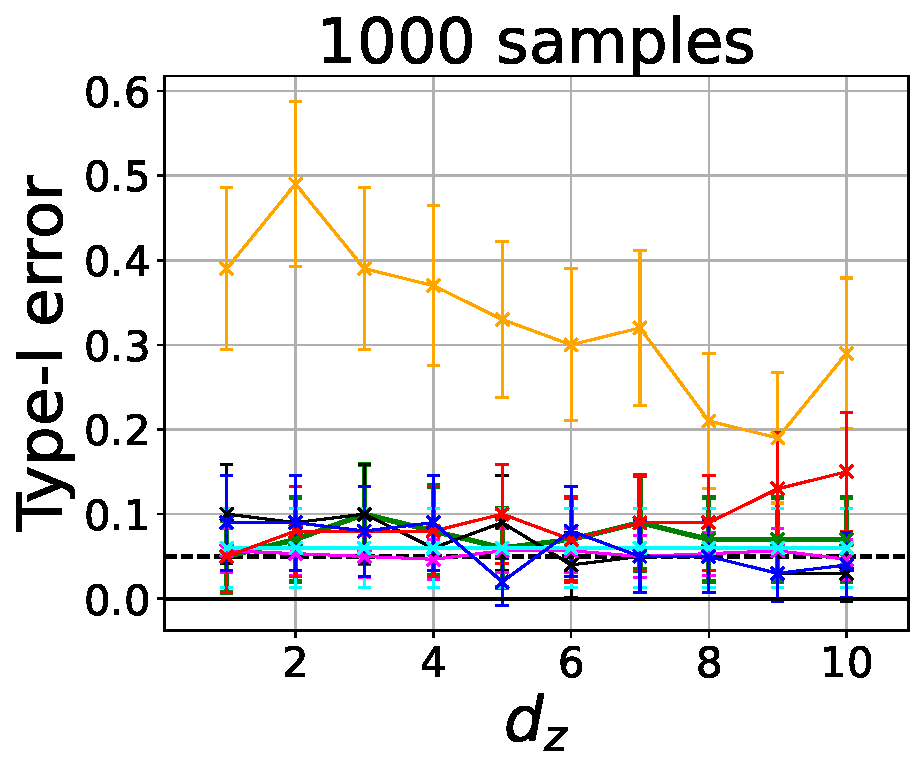
\includegraphics[height=2.2cm]{sections/appendix/independence_testing_kernel/figures_strobl_gaussian/nsamples_fixed_1000_strobl_dim_1_10_typeI.pdf}& 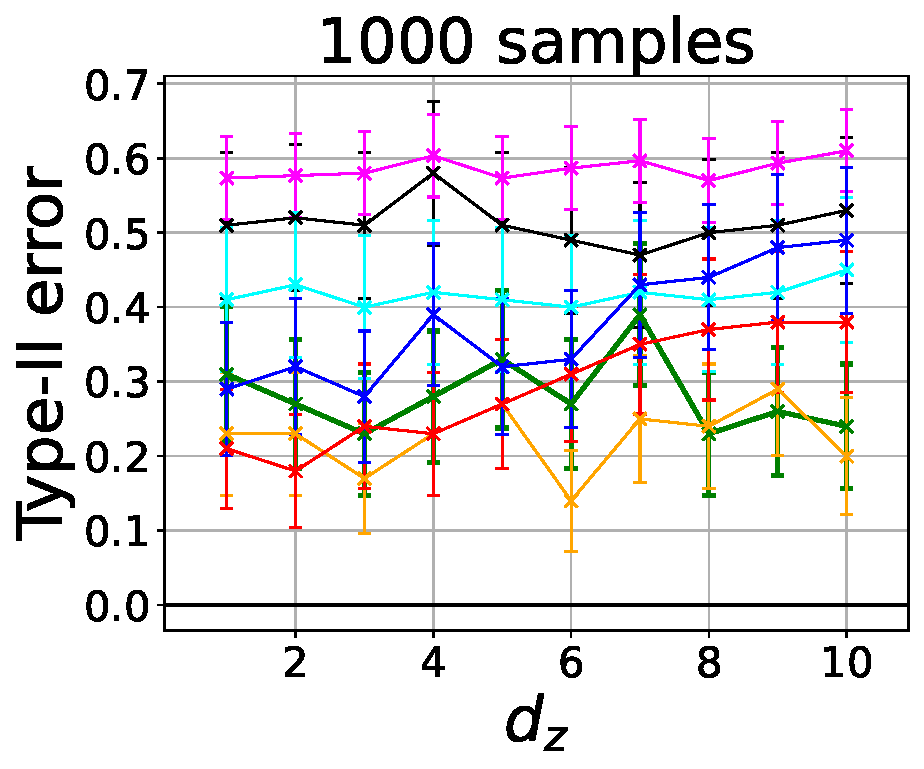
\includegraphics[height=2.2cm]{sections/appendix/independence_testing_kernel/figures_strobl_gaussian/nsamples_fixed_1000_strobl_dim_1_10_typeII.pdf} & 
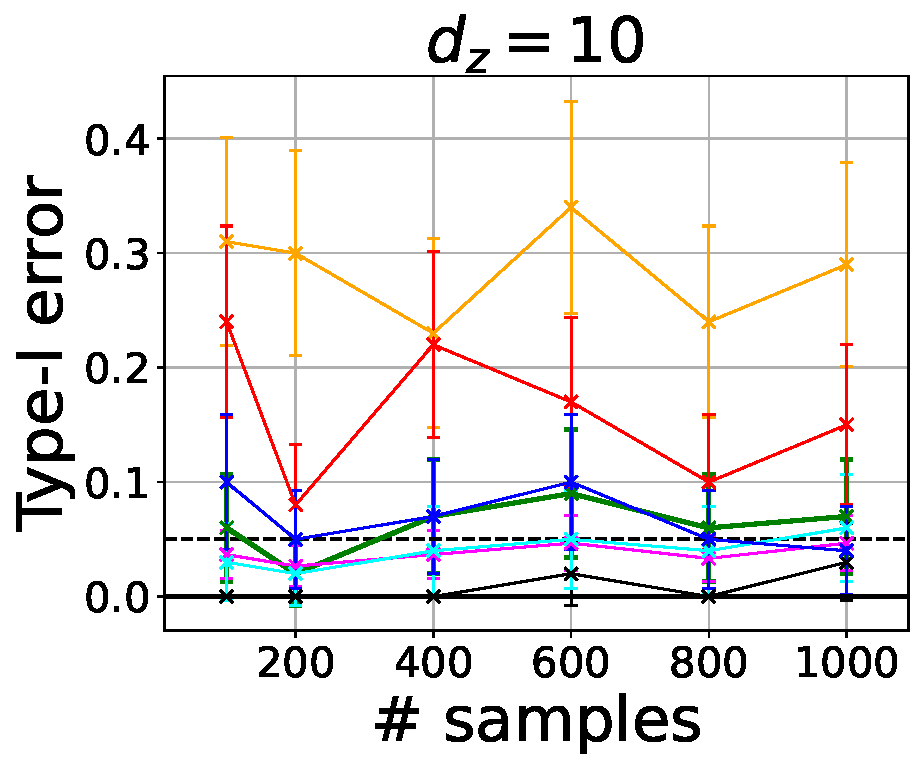
\includegraphics[height=2.2cm]{sections/appendix/independence_testing_kernel/figures_strobl_gaussian/dim_fixed_10_strobl_typeI.pdf}& 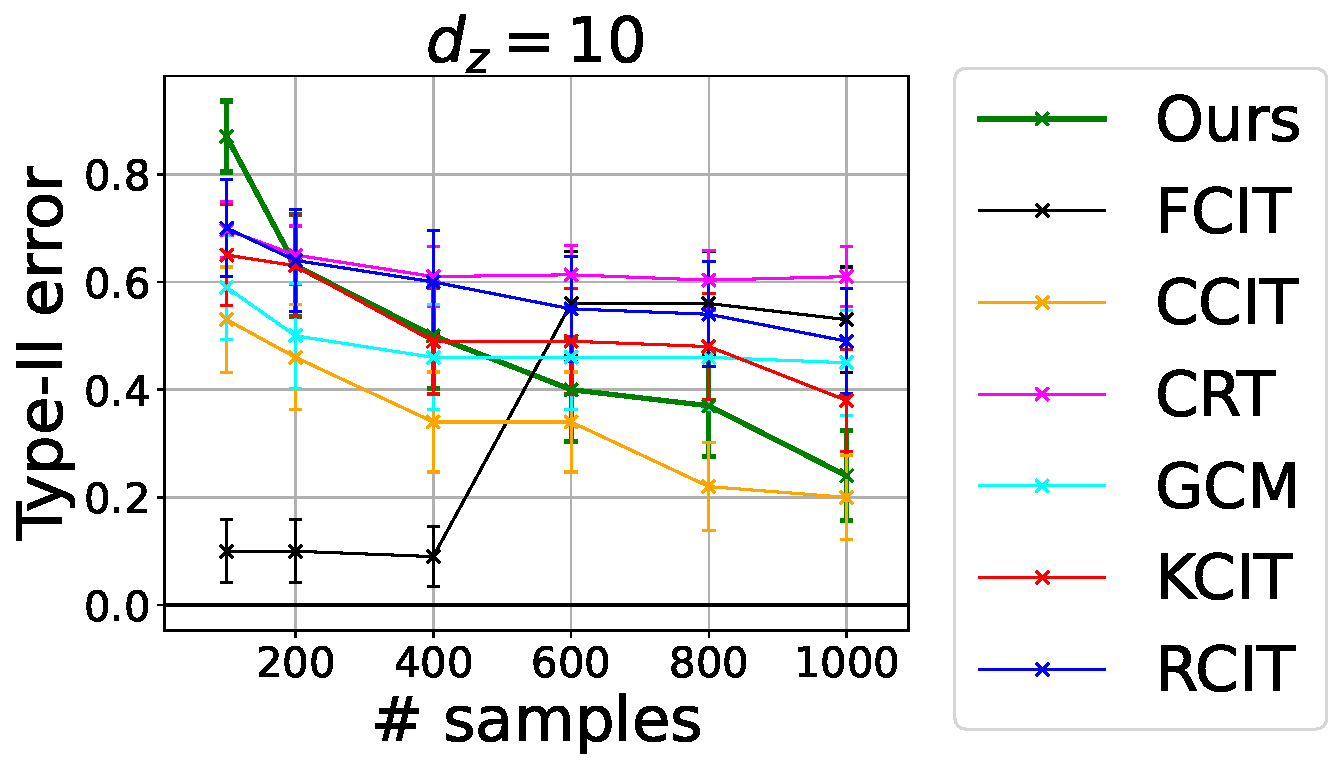
\includegraphics[height=2.2cm]{sections/appendix/independence_testing_kernel/figures_strobl_gaussian/dim_fixed_10_strobl_typeII.pdf}
\end{tabular}
\caption{Comparison of the type-I error at level $\alpha=0.05$ (dashed line) and the type-II error (lower is better) of our test procedure with other SoTA tests on the two problems presented in~\eqref{exp-strobl-h0} and~\eqref{exp-strobl-h1}  with Gaussian noises. Each point in the figures is obtained by repeating the experiment for 100 independent trials. (\emph{Left, middle-left}): type-I and type-II errors obtained by each test when varying the dimension $d_z$ from 1 to 10; here, the number of samples $n$ is fixed and equals to $1000$. (\emph{Middle-right, right}): type-I and type-II errors obtained by each test when varying the number of samples $n$ from 100 to 1000; the dimension $d_z$ is fixed and equals $10$. 
\label{fig-exp-strobl-type-supp}}
\vspace{-0.5cm}
\end{figure*}




\begin{figure*}[ht]
\begin{tabular}{cccc} 
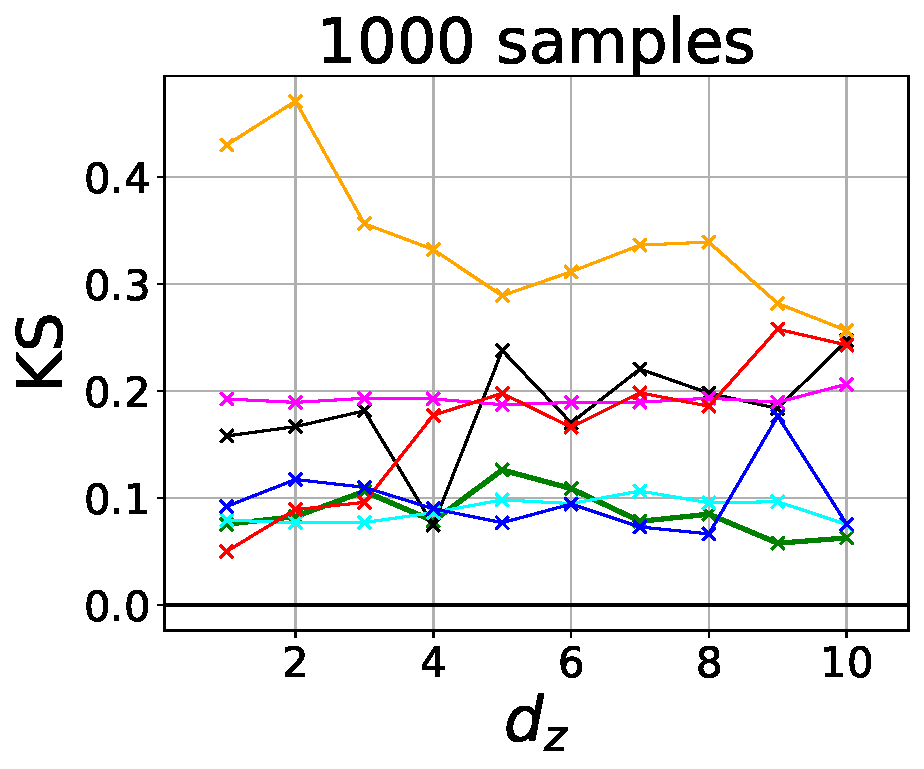
\includegraphics[height=2.2cm]{sections/appendix/independence_testing_kernel/new_figures/nsamples_fixed_1000_strobl_dim_1_10_ks.pdf}& 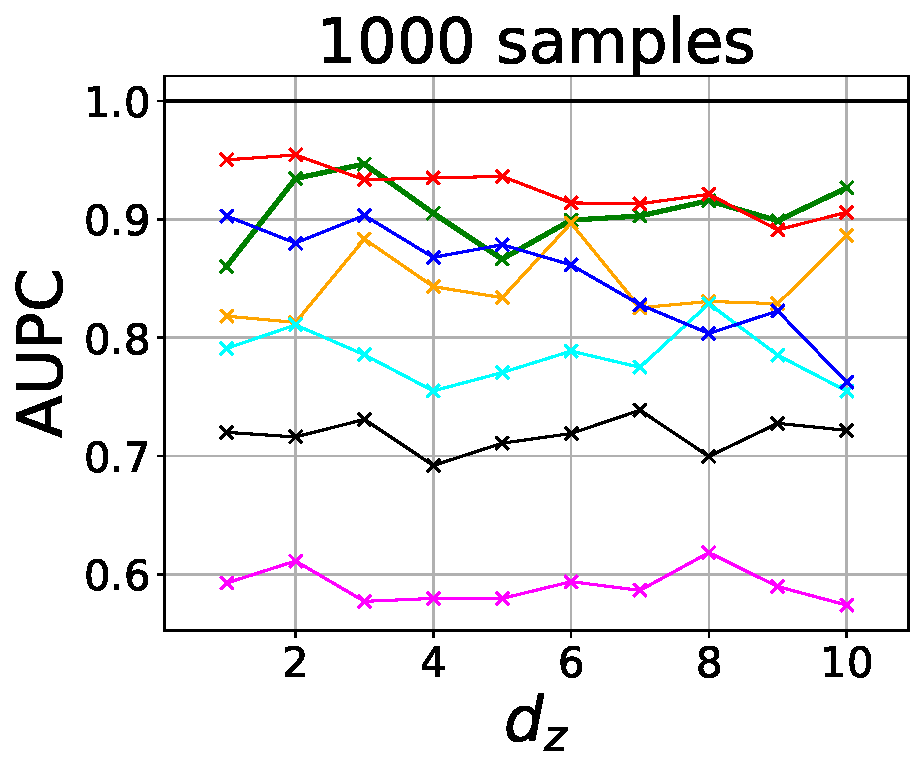
\includegraphics[height=2.2cm]{sections/appendix/independence_testing_kernel/new_figures/nsamples_fixed_1000_strobl_dim_1_10_aupc.pdf} & 
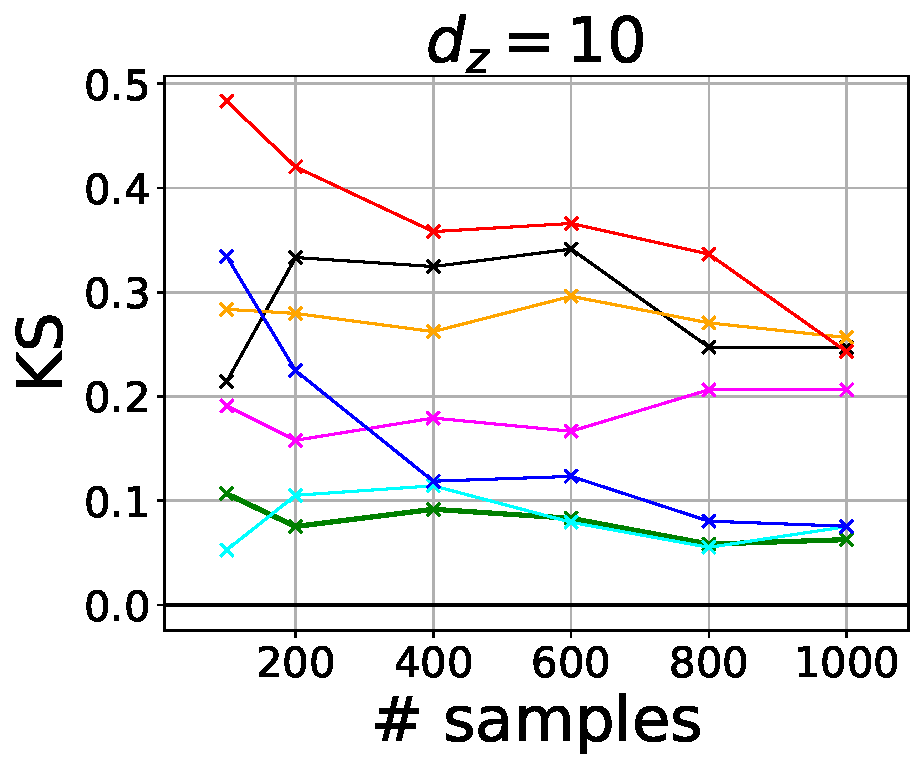
\includegraphics[height=2.2cm]{sections/appendix/independence_testing_kernel/new_figures/dim_fixed_10_strobl_ks.pdf}& 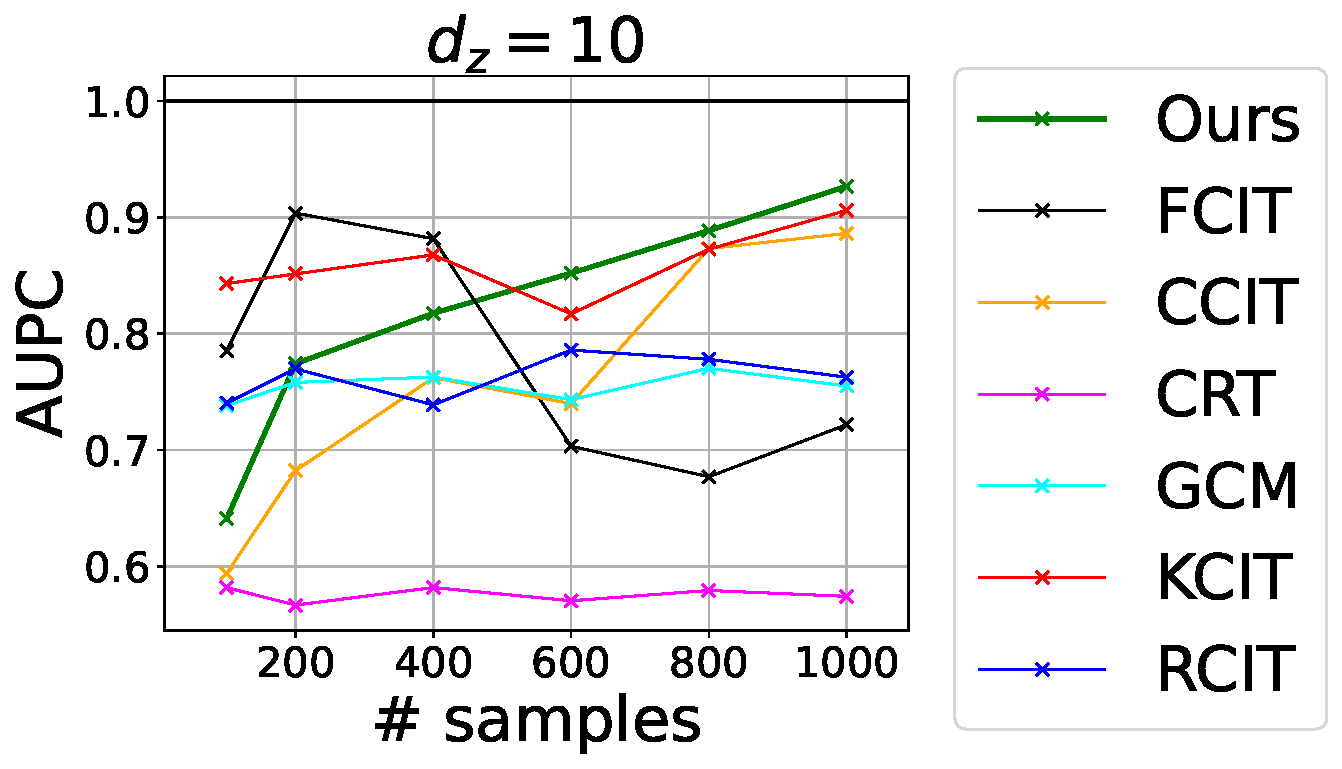
\includegraphics[height=2.2cm]{sections/appendix/independence_testing_kernel/new_figures/dim_fixed_10_strobl_aupc.pdf} 
\end{tabular}
\caption{Comparison of the KS statistic (lower is better) and the AUPC (higher is better) of our testing procedure with other SoTA tests on the two problems presented in~\eqref{exp-strobl-h0} and~\eqref{exp-strobl-h1}  with Gaussian noises. Each point in the figures is obtained by repeating the experiment forx 100 independent trials. (\emph{Left, middle-left}): the KS and AUPC obtained by each test when varying the dimension $d_z$ from 1 to 10, while fixing the number of samples $n$ to $1000$. (\emph{Middle-right, right}): the KS and AUPC obtained by each test when varying the number of samples $n$ from 100 to 1000, while fixing the dimension $d_z$ to $10$. 
\label{fig-exp-strobl-ks-supp}}
\vspace{-0.5cm}
\end{figure*}




\begin{figure*}[h]
\begin{tabular}{cccc} 
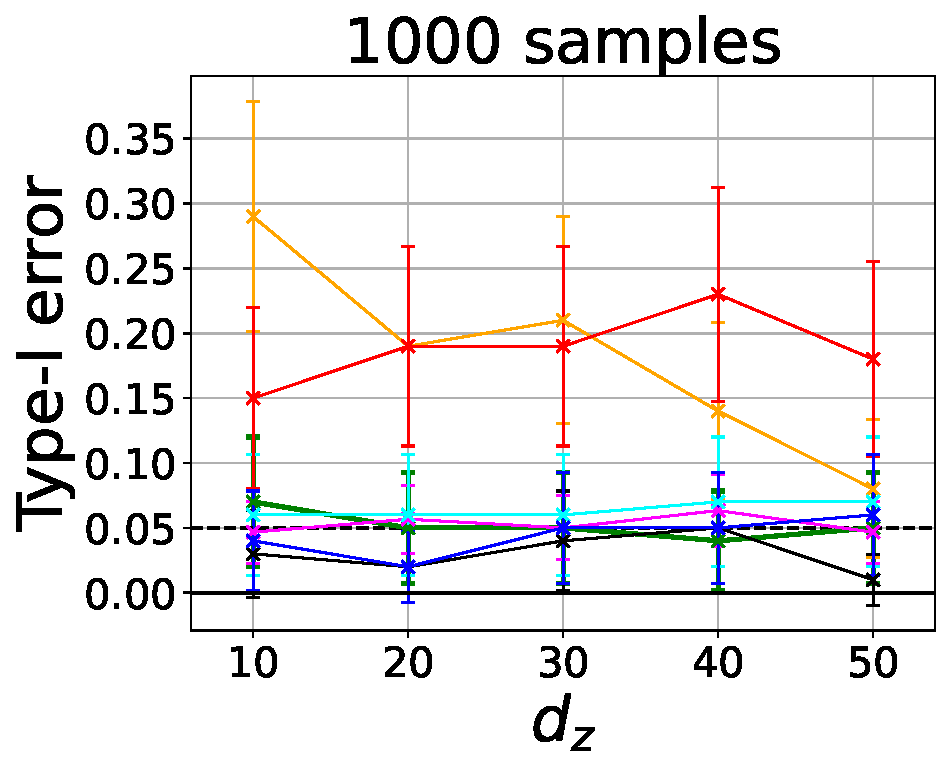
\includegraphics[height=2.2cm]{sections/appendix/independence_testing_kernel/figures_strobl_highdim_gaussian/nsamples_fixed_1000_strobl_dim_10_50_typeI.pdf}& 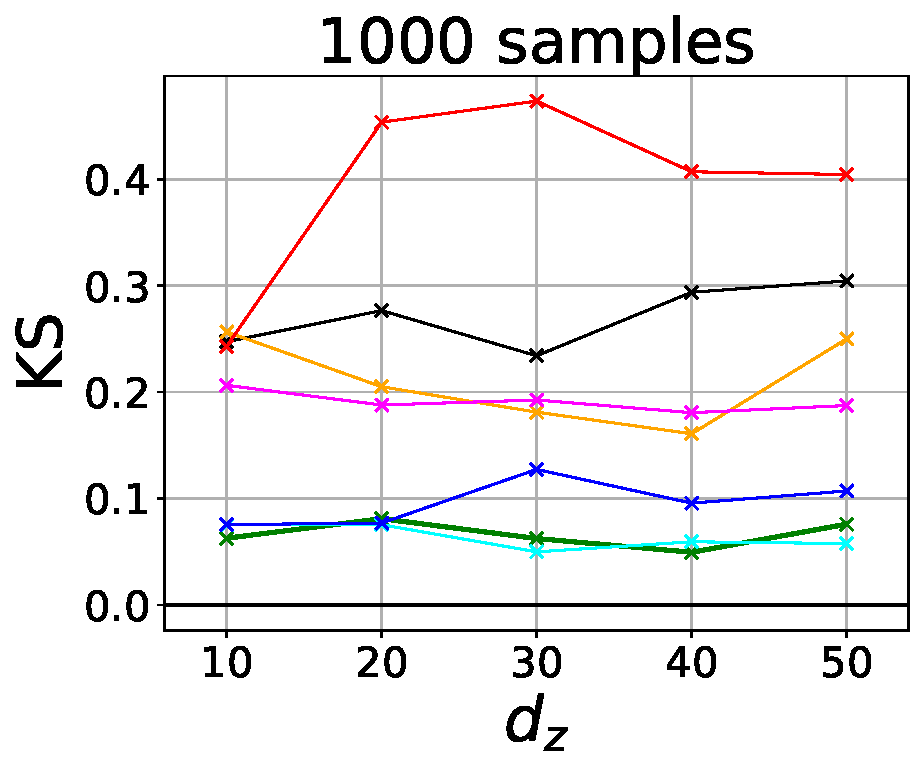
\includegraphics[height=2.2cm]{sections/appendix/independence_testing_kernel/figures_strobl_highdim_gaussian/nsamples_fixed_1000_strobl_dim_10_50_ks.pdf} & 
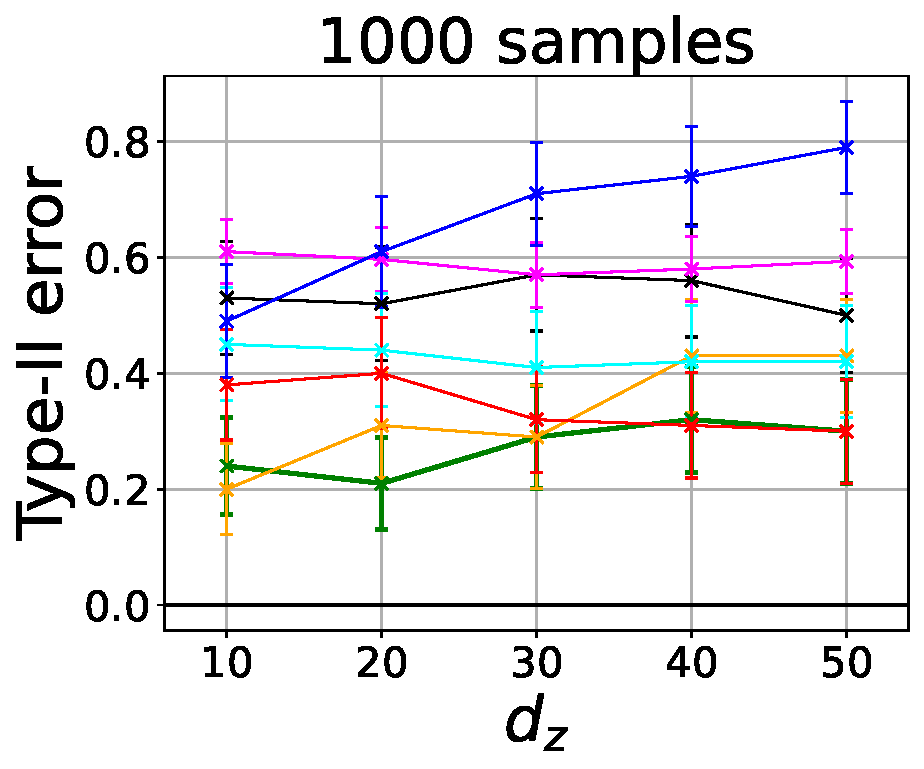
\includegraphics[height=2.2cm]{sections/appendix/independence_testing_kernel/figures_strobl_highdim_gaussian/nsamples_fixed_1000_strobl_dim_10_50_typeII.pdf}& 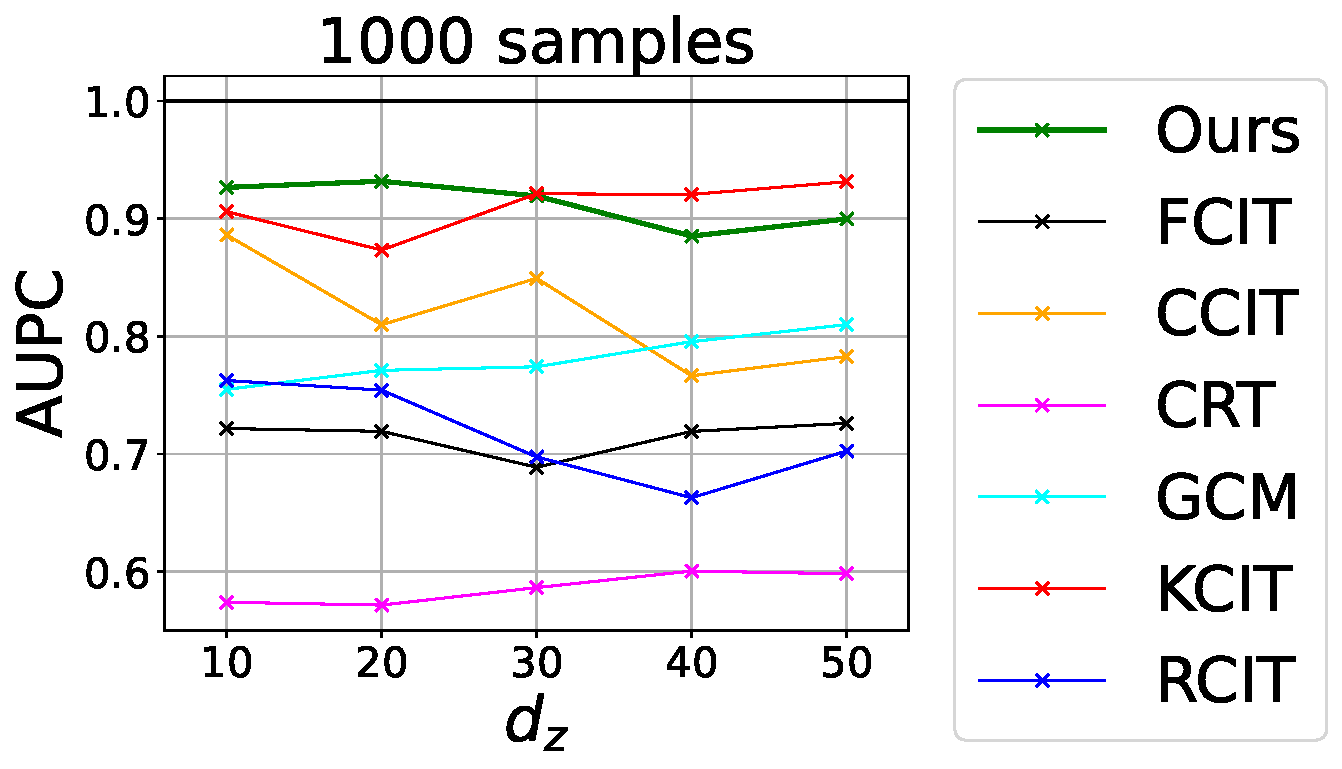
\includegraphics[height=2.2cm]{sections/appendix/independence_testing_kernel/figures_strobl_highdim_gaussian/nsamples_fixed_1000_strobl_dim_10_50_aupc.pdf}
\end{tabular}
\caption{Comparison of the type-I error at level $\alpha=0.05$ (dashed line), type-II error (lower is better), KS statistic and the AUPC of our testing procedure with other SoTA tests on the two problems presented in Eq.~\eqref{exp-strobl-h0} and Eq.~\eqref{exp-strobl-h1} with Gaussian noises. Each point in the figures is obtained by repeating the experiment for 100 independent trials. In each plot the dimension $d_z$ is varying from 10 to 50; here, the number of samples $n$ is fixed and equals to $1000$. 
\label{fig-exp-strobl-highdim-gaussian-supp}}
\vspace{-0.6cm}
\end{figure*}











\newpage


\subsubsection{Laplace Case}
\vspace{-0.4cm}






\begin{figure*}[htb]
\begin{tabular}{cccc} 
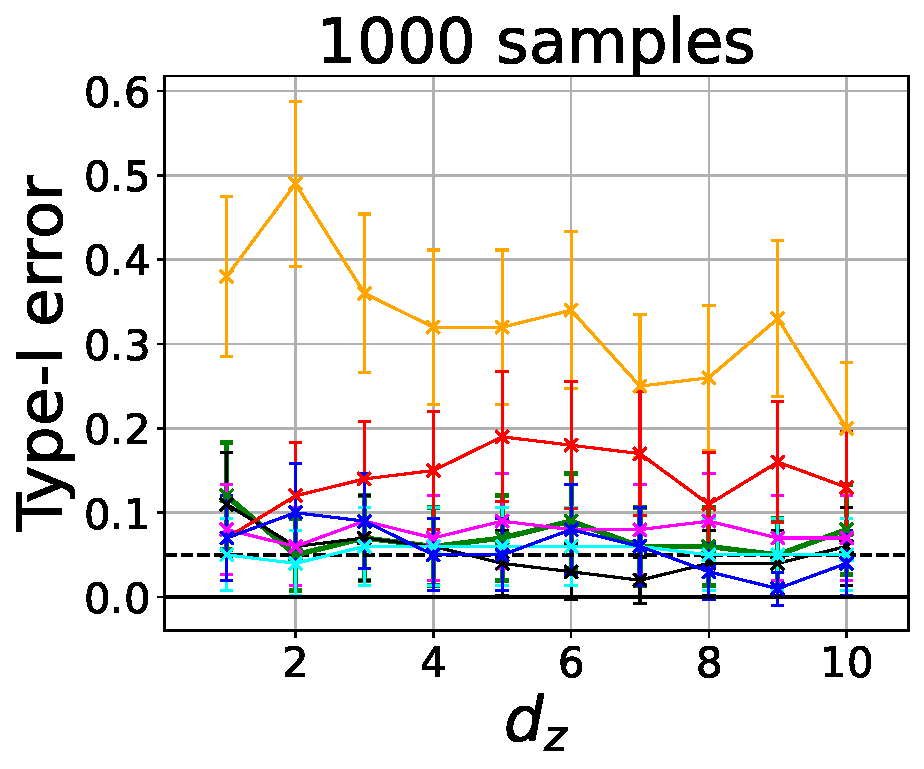
\includegraphics[height=2.2cm]{sections/appendix/independence_testing_kernel/new_figures_lap/nsamples_fixed_1000_strobl_dim_1_10_typeI.pdf}& 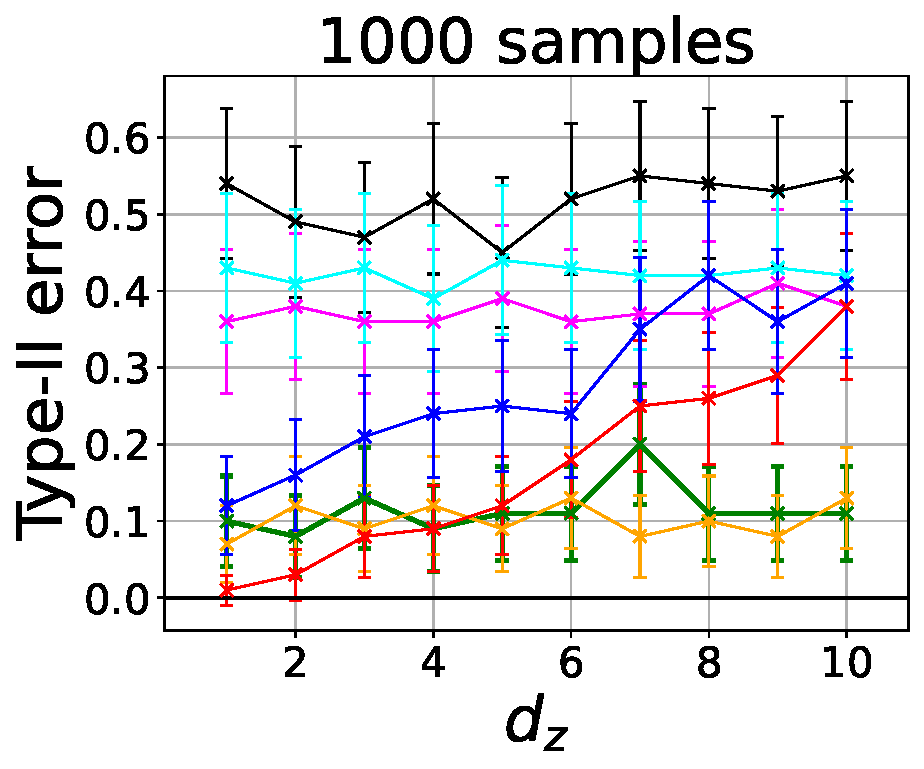
\includegraphics[height=2.2cm]{sections/appendix/independence_testing_kernel/new_figures_lap/nsamples_fixed_1000_strobl_dim_1_10_typeII.pdf} & 
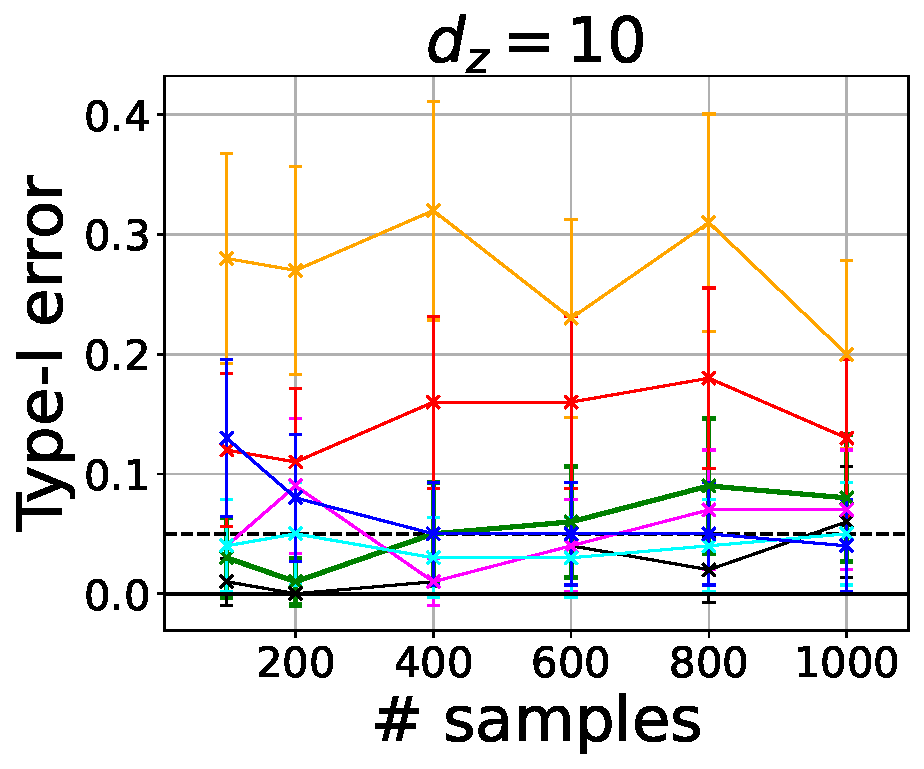
\includegraphics[height=2.2cm]{sections/appendix/independence_testing_kernel/new_figures_lap/dim_fixed_10_strobl_typeI.pdf}& 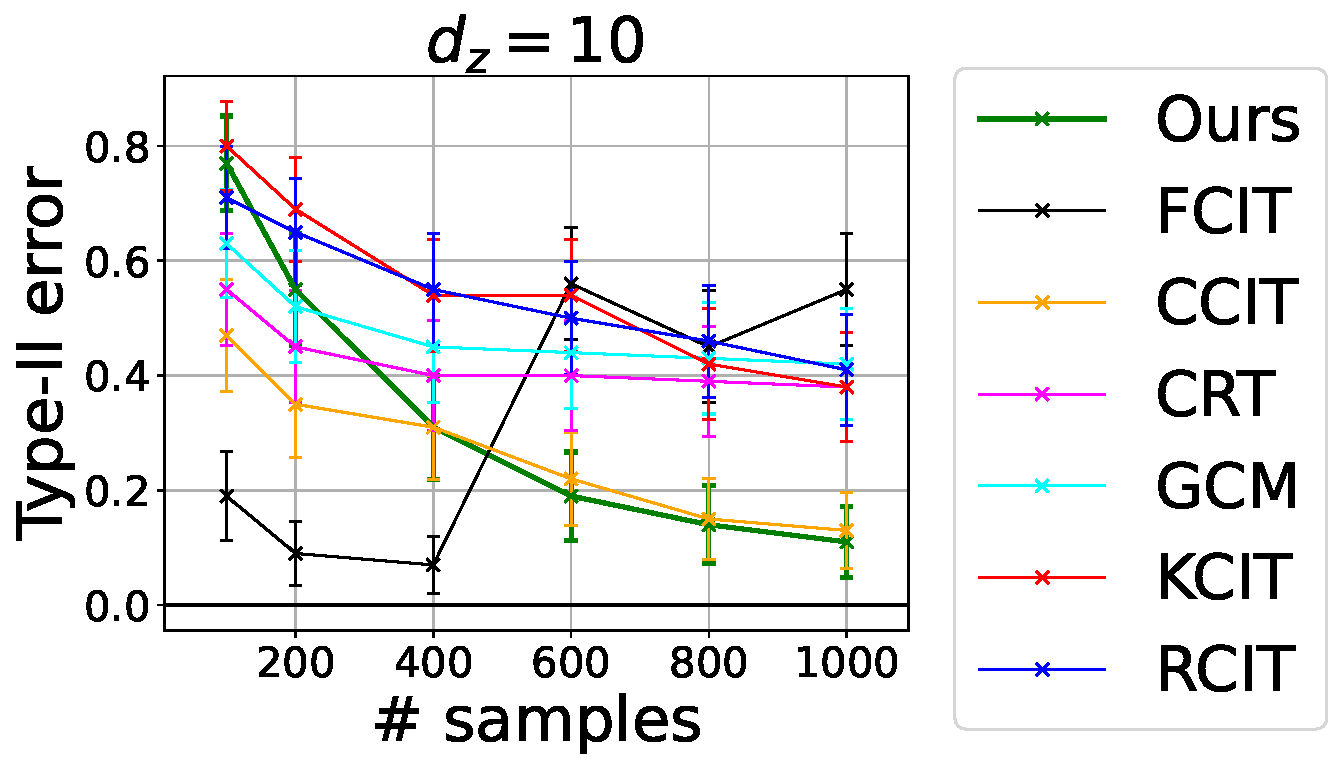
\includegraphics[height=2.2cm]{sections/appendix/independence_testing_kernel/new_figures_lap/dim_fixed_10_strobl_typeII.pdf} 
\end{tabular}
\caption{Comparison of the type-I error at level $\alpha=0.05$ (dashed line) and the type-II error (lower is better) of our test procedure with other SoTA tests on the two problems presented in~\eqref{exp-strobl-h0} and~\eqref{exp-strobl-h1} with Laplace noises. Each point in the figures is obtained by repeating the experiment for 100 independent trials. (\emph{Left, middle-left}): type-I and type-II errors obtained by each test when varying the dimension $d_z$ from 1 to 10; here, the number of samples $n$ is fixed and equals to $1000$. (\emph{Middle-right, right}): type-I and type-II errors obtained by each test when varying the number of samples $n$ from 100 to 1000; here, the dimension $d_z$ is fixed and equals to $10$.
\label{fig-exp-strobl-laplace-supp}}
\vspace{-0.5cm}
\end{figure*}




\begin{figure*}[htb]
\begin{tabular}{cccc} 
\includegraphics[height=2.2cm]{sections/appendix/independence_testing_kernel/new_figures_lap/nsamples_fixed_1000_strobl_dim_1_10_ks.pdf}& \includegraphics[height=2.2cm]{sections/appendix/independence_testing_kernel/new_figures_lap/nsamples_fixed_1000_strobl_dim_1_10_aupc.pdf} & 
\includegraphics[height=2.2cm]{sections/appendix/independence_testing_kernel/new_figures_lap/dim_fixed_10_strobl_ks.pdf}& \includegraphics[height=2.2cm]{sections/appendix/independence_testing_kernel/new_figures_lap/dim_fixed_10_strobl_aupc.pdf} 
\end{tabular}
\caption{Comparison of the KS statistic and the AUPC of our testing procedure with other SoTA tests on the two problems presented in Eq.~\eqref{exp-strobl-h0} and Eq.~\eqref{exp-strobl-h1}  with Laplace noises. Each point in the figures is obtained by repeating the experiment for 100 independent trials. (\emph{Left, middle-left}): the KS statistic and AUPC (respectively) obtained by each test when varying the dimension $d_z$ from 1 to 10; here, the number of samples $n$ is fixed and equals to $1000$. (\emph{Middle-right, right}): the KS and AUPC (respectively), obtained by each test when varying the number of samples $n$ from 100 to 1000; here, the dimension $d_z$ is fixed and equals to $10$.
\label{fig-exp-strobl-ks-laplace-supp}}
\vspace{-0.5cm}
\end{figure*}


\begin{figure*}[ht]
\begin{tabular}{cccc} 
\includegraphics[height=2.2cm]{sections/appendix/independence_testing_kernel/figures_strobl_highdim_lap/nsamples_fixed_1000_strobl_dim_10_50_typeI.pdf}& \includegraphics[height=2.2cm]{sections/appendix/independence_testing_kernel/figures_strobl_highdim_lap/nsamples_fixed_1000_strobl_dim_10_50_ks.pdf} & 
\includegraphics[height=2.2cm]{sections/appendix/independence_testing_kernel/figures_strobl_highdim_lap/nsamples_fixed_1000_strobl_dim_10_50_typeII.pdf}& \includegraphics[height=2.2cm]{sections/appendix/independence_testing_kernel/figures_strobl_highdim_lap/nsamples_fixed_1000_strobl_dim_10_50_aupc.pdf}
\end{tabular}
\caption{Comparison of the type-I error at level $\alpha=0.05$ (dashed line), type-II error (lower is better), KS statistic and the AUPC of our testing procedure with other SoTA tests on the two problems presented in Eq.~\eqref{exp-strobl-h0} and Eq.~\eqref{exp-strobl-h1} with Laplace noises. Each point in the figures is obtained by repeating the experiment for 100 independent trials. In each plot the dimension $d_z$ is varying from 10 to 50; here, the number of samples $n$ is fixed and equals to $1000$.
\label{fig-exp-strobl-highdim-laplace-supp}}
\vspace{-0.8cm}
\end{figure*}


\newpage
\subsection{Additional experiments on Problems~\eqref{li-exp-h0} and~\eqref{li-exp-h1}}
\label{sec-exp-li}
\vspace{-0.2cm}
\subsubsection{Gaussian Case}
\vspace{-0.4cm}


% Figure~\ref{fig-exp-li-ks-gauss} compares the KS statistic and the AUPC obtained by different testing procedures in the exact same setting considered in Figure~\ref{fig-exp-li}. Following that figure, one can see that our method outperforms the other tests both in terms of type-I error and power. In addition, Figure~\ref{fig-exp-li-ks-highdim} presets the results obtained in a high dimensional regime, showing that our method tends to outperform the existing tests in most cases.


\begin{figure*}[htb]
\begin{tabular}{cccc} 
\includegraphics[height=2.2cm]{sections/appendix/independence_testing_kernel/new_figures/nsamples_fixed_1000_li_dim_1_10_typeI.pdf}& \includegraphics[height=2.2cm]{sections/appendix/independence_testing_kernel/new_figures/nsamples_fixed_1000_li_dim_1_10_typeII.pdf} & 
\includegraphics[height=2.2cm]{sections/appendix/independence_testing_kernel/new_figures/dim_fixed_10_li_typeI.pdf}& \includegraphics[height=2.2cm]{sections/appendix/independence_testing_kernel/new_figures/dim_fixed_10_li_typeII.pdf} 
\end{tabular}
\caption{Comparison of the type-I error at level $\alpha=0.05$ (dashed line) and the type-II error (lower is better) of our test procedure with other SoTA tests on the two problems presented in~\eqref{li-exp-h0} and~\eqref{li-exp-h1}  with Gaussian noises. Each point in the figures is obtained by repeating the experiment for 100 independent trials. (\emph{Left, middle-left}): type-I and type-II errors obtained by each test when varying the dimension $d_z$ from 1 to 10; here, the number of samples $n$ is fixed and equals to $1000$. (\emph{Middle-right, right}): type-I and type-II errors obtained by each test when varying the number of samples $n$ from 100 to 1000; here, the dimension $d_z$ is fixed and equals to $10$. 
\label{fig-exp-li-type-supp}}
\vspace{-0.5cm}
\end{figure*}


\begin{figure*}[ht]
\begin{tabular}{cccc} 
\includegraphics[height=2.2cm]{sections/appendix/independence_testing_kernel/figures_supp_mat/nsamples_fixed_1000_li_dim_1_10_ks.pdf}& \includegraphics[height=2.2cm]{sections/appendix/independence_testing_kernel/figures_supp_mat/nsamples_fixed_1000_li_dim_1_10_aupc.pdf} & 
\includegraphics[height=2.2cm]{sections/appendix/independence_testing_kernel/figures_supp_mat/dim_fixed_10_li_ks.pdf}& \includegraphics[height=2.2cm]{sections/appendix/independence_testing_kernel/figures_supp_mat/dim_fixed_10_li_aupc.pdf}
\end{tabular}
\caption{Comparison of the KS statistic and the AUPC of our testing procedure with other SoTA tests on the two problems presented in Eq.~\eqref{li-exp-h0} and Eq.~\eqref{li-exp-h1} with Gaussian noises. Each point in the figures is obtained by repeating the experiment for 100 independent trials. (\emph{Left, middle-left}): the KS statistic and AUPC (respectively) obtained by each test when varying the dimension $d_z$ from 1 to 10; here, the number of samples $n$ is fixed and equals to $1000$. (\emph{Middle-right, right}): the KS and AUPC (respectively), obtained by each test when varying the number of samples $n$ from 100 to 1000; the dimension $d_z$ is fixed and equals $10$.
\label{fig-exp-li-ks-gauss-supp}}
\vspace{-0.8cm}
\end{figure*}


\begin{figure*}[ht]
\begin{tabular}{cccc} 
\includegraphics[height=2.2cm]{sections/appendix/independence_testing_kernel/figures_li_highdim/nsamples_fixed_1000_li_dim_10_50_typeI.pdf}& \includegraphics[height=2.2cm]{sections/appendix/independence_testing_kernel/figures_li_highdim/nsamples_fixed_1000_li_dim_10_50_ks.pdf} & 
\includegraphics[height=2.2cm]{sections/appendix/independence_testing_kernel/figures_li_highdim/nsamples_fixed_1000_li_dim_10_50_typeII.pdf}& \includegraphics[height=2.2cm]{sections/appendix/independence_testing_kernel/figures_li_highdim/nsamples_fixed_1000_li_dim_10_50_aupc.pdf}
\end{tabular}
\caption{Comparison of the type-I error at level $\alpha=0.05$ (dashed line), type-II error (lower is better), KS statistic and the AUPC of our testing procedure with other SoTA tests on the two problems presented in Eq.~\eqref{li-exp-h0} and Eq.~\eqref{li-exp-h1} with Gaussian noises. Each point in the figures is obtained by repeating the experiment for 100 independent trials. In each plot the dimension $d_z$ is varying from 10 to 50; here, the number of samples $n$ is fixed and equals to $1000$. 
\label{fig-exp-li-highdim-gauss-supp}}
\vspace{-0.8cm}
\end{figure*}


\newpage
\subsubsection{Laplace Case}
\vspace{-0.4cm}
\begin{figure*}[h]
\begin{tabular}{cccc} 
\includegraphics[height=2.2cm]{sections/appendix/independence_testing_kernel/new_figures_lap/nsamples_fixed_1000_li_dim_1_10_typeI.pdf}& \includegraphics[height=2.2cm]{sections/appendix/independence_testing_kernel/new_figures_lap/nsamples_fixed_1000_li_dim_1_10_typeII.pdf} & 
\includegraphics[height=2.2cm]{sections/appendix/independence_testing_kernel/new_figures_lap/dim_fixed_10_li_typeI.pdf}& \includegraphics[height=2.2cm]{sections/appendix/independence_testing_kernel/new_figures_lap/dim_fixed_10_li_typeII.pdf} 
\end{tabular}
\caption{Comparison of the type-I error at level $\alpha=0.05$ (dashed line) and the type-II error (lower is better) of our test procedure with other SoTA tests on the two problems presented in~\eqref{li-exp-h0} and~\eqref{li-exp-h1}  with Laplace noises. Each point in the figures is obtained by repeating the experiment for 100 independent trials. (\emph{Left, middle-left}): type-I and type-II errors obtained by each test when varying the dimension $d_z$ from 1 to 10; here, the number of samples $n$ is fixed and equals to $1000$. (\emph{Middle-right, right}): type-I and type-II errors obtained by each test when varying the number of samples $n$ from 100 to 1000; the dimension $d_z$ is fixed and equals $10$. 
\label{fig-exp-li-laplace-supp}}
\vspace{-0.5cm}
\end{figure*}

\begin{figure*}[h]
\begin{tabular}{cccc} 
\includegraphics[height=2.2cm]{sections/appendix/independence_testing_kernel/new_figures_lap/nsamples_fixed_1000_li_dim_1_10_ks.pdf}& \includegraphics[height=2.2cm]{sections/appendix/independence_testing_kernel/new_figures_lap/nsamples_fixed_1000_li_dim_1_10_aupc.pdf} & 
\includegraphics[height=2.2cm]{sections/appendix/independence_testing_kernel/new_figures_lap/dim_fixed_10_li_ks.pdf}& \includegraphics[height=2.2cm]{sections/appendix/independence_testing_kernel/new_figures_lap/dim_fixed_10_li_aupc.pdf} 
\end{tabular}
\caption{Comparison of the KS statistic and the AUPC of our testing procedure with other SoTA tests on the two problems presented in Eq.~\eqref{li-exp-h0} and Eq.~\eqref{li-exp-h1}  with Laplace noises. Each point in the figures is obtained by repeating the experiment for 100 independent trials. (\emph{Left, middle-left}): the KS statistic and AUPC (respectively) obtained by each test when varying the dimension $d_z$ from 1 to 10; here, the number of samples $n$ is fixed and equals to $1000$. (\emph{Middle-right, right}): the KS and AUPC (respectively), obtained by each test when varying the number of samples $n$ from 100 to 1000; the dimension $d_z$ is fixed and equals $10$.
\label{fig-exp-li-ks-laplace-supp}}
\vspace{-0.5cm}
\end{figure*}


\begin{figure*}[h]
\begin{tabular}{cccc} 
\includegraphics[height=2.2cm]{sections/appendix/independence_testing_kernel/figures_li_highdim_lap/nsamples_fixed_1000_li_dim_10_50_typeI.pdf}& \includegraphics[height=2.2cm]{sections/appendix/independence_testing_kernel/figures_li_highdim_lap/nsamples_fixed_1000_li_dim_10_50_ks.pdf} & 
\includegraphics[height=2.2cm]{sections/appendix/independence_testing_kernel/figures_li_highdim_lap/nsamples_fixed_1000_li_dim_10_50_typeII.pdf}& \includegraphics[height=2.2cm]{sections/appendix/independence_testing_kernel/figures_li_highdim_lap/nsamples_fixed_1000_li_dim_10_50_aupc.pdf}
\end{tabular}
\caption{Comparison of the type-I error at level $\alpha=0.05$ (dashed line), type-II error (lower is better), KS statistic and the AUPC of our testing procedure with other SoTA tests on the two problems presented in Eq.~\eqref{li-exp-h0} and Eq.~\eqref{li-exp-h1} with Laplace noises. Each point in the figures is obtained by repeating the experiment for 100 independent trials. In each plot the dimension $d_z$ is varying from 10 to 50; here, the number of samples $n$ is fixed and equals to $1000$. 
\label{fig-exp-li-highdim-laplace-supp}}
\vspace{-0.8cm}
\end{figure*}










% \subsection{Additional experiments on Problems~\eqref{exp-strobl-h0} and~\eqref{exp-strobl-h1}}
% \label{sec-exp-storbl}

% \subsubsection{Gaussian Case}
% % In this section, we provide an additional comparison of the KS statistic and the AUPC obtained by the different tests when the data is generated from the models defined in Eq.~\eqref{exp-strobl-h0} and Eq.~\eqref{exp-strobl-h1}, respectively, focusing on a high dimensional setting. Figure~\ref{fig-exp-li-ks-dim} demonstrates that, in most cases, our method indeed outperforms the existing tests both in terms of the KS and AUPC performance metrics.


% \begin{figure*}[h]
% \begin{tabular}{cccc} 
% \includegraphics[height=2.2cm]{figures_strobl_gaussian/nsamples_fixed_1000_strobl_dim_1_10_typeI.pdf}& \includegraphics[height=2.2cm]{figures_strobl_gaussian/nsamples_fixed_1000_strobl_dim_1_10_typeII.pdf} & 
% \includegraphics[height=2.2cm]{figures_strobl_gaussian/dim_fixed_10_strobl_typeI.pdf}& \includegraphics[height=2.2cm]{figures_strobl_gaussian/dim_fixed_10_strobl_typeII.pdf}
% \end{tabular}
% \caption{Comparison of the type-I error at level $\alpha=0.05$ (dashed line) and the type-II error (lower is better) of our test procedure with other SoTA tests on the two problems presented in~\eqref{exp-strobl-h0} and~\eqref{exp-strobl-h1}  with Gaussian noises. Each point in the figures is obtained by repeating the experiment for 100 independent trials. (\emph{Left, middle-left}): type-I and type-II errors obtained by each test when varying the dimension $d_z$ from 1 to 10; here, the number of samples $n$ is fixed and equals to $1000$. (\emph{Middle-right, right}): type-I and type-II errors obtained by each test when varying the number of samples $n$ from 100 to 1000; here, the dimension $d_z$ is fixed and equals to $10$. 
% \label{fig-exp-strobl-type-supp}}
% \vspace{-0.5cm}
% \end{figure*}




% \begin{figure*}[ht]
% \begin{tabular}{cccc} 
% \includegraphics[height=2.2cm]{new_figures/nsamples_fixed_1000_strobl_dim_1_10_ks.pdf}& \includegraphics[height=2.2cm]{new_figures/nsamples_fixed_1000_strobl_dim_1_10_aupc.pdf} & 
% \includegraphics[height=2.2cm]{new_figures/dim_fixed_10_strobl_ks.pdf}& \includegraphics[height=2.2cm]{new_figures/dim_fixed_10_strobl_aupc.pdf} 
% \end{tabular}
% \caption{Comparison of the KS statistic (lower is better) and the AUPC (higher is better) of our testing procedure with other SoTA tests on the two problems presented in~\eqref{exp-strobl-h0} and~\eqref{exp-strobl-h1}  with Gaussian noises. Each point in the figures is obtained by repeating the experiment for 100 independent trials. (\emph{Left, middle-left}): the KS and AUPC obtained by each test when varying the dimension $d_z$ from 1 to 10, while fixing the number of samples $n$ to $1000$. (\emph{Middle-right, right}): the KS and AUPC obtained by each test when varying the number of samples $n$ from 100 to 1000, while fixing the dimension $d_z$ to $10$. These experiments show that our method outperforms other tests both in term of KS and AUPC in most of the settings.
% \label{fig-exp-strobl-supp}}
% \vspace{-0.5cm}
% \end{figure*}




% \begin{figure*}[h]
% \begin{tabular}{cccc} 
% \includegraphics[height=2.2cm]{figures_strobl_highdim_gaussian/nsamples_fixed_1000_strobl_dim_10_50_typeI.pdf}& \includegraphics[height=2.2cm]{figures_strobl_highdim_gaussian/nsamples_fixed_1000_strobl_dim_10_50_ks.pdf} & 
% \includegraphics[height=2.2cm]{figures_strobl_highdim_gaussian/nsamples_fixed_1000_strobl_dim_10_50_typeII.pdf}& \includegraphics[height=2.2cm]{figures_strobl_highdim_gaussian/nsamples_fixed_1000_strobl_dim_10_50_aupc.pdf}
% \end{tabular}
% \caption{Comparison of the type-I error at level $\alpha=0.05$ (dashed line), type-II error (lower is better), KS statistic and the AUPC of our testing procedure with other SoTA tests on the two problems presented in Eq.~\eqref{exp-strobl-h0} and Eq.~\eqref{exp-strobl-h1} with Gaussian noises. Each point in the figures is obtained by repeating the experiment for 100 independent trials. In each plot the dimension $d_z$ is varying from 10 to 50; here, the number of samples $n$ is fixed and equals to $1000$. 
% \label{fig-exp-strobl-highdim-gaussian-supp}}
% \vspace{-0.5cm}
% \end{figure*}









% \newpage


% \subsubsection{Laplace Case}







% \begin{figure*}[htb]
% \begin{tabular}{cccc} 
% \includegraphics[height=2.2cm]{new_figures_lap/nsamples_fixed_1000_strobl_dim_1_10_typeI.pdf}& \includegraphics[height=2.2cm]{new_figures_lap/nsamples_fixed_1000_strobl_dim_1_10_typeII.pdf} & 
% \includegraphics[height=2.2cm]{new_figures_lap/dim_fixed_10_strobl_typeI.pdf}& \includegraphics[height=2.2cm]{new_figures_lap/dim_fixed_10_strobl_typeII.pdf} 
% \end{tabular}
% \caption{Comparison of the type-I error at level $\alpha=0.05$ (dashed line) and the type-II error (lower is better) of our test procedure with other SoTA tests on the two problems presented in~\eqref{exp-strobl-h0} and~\eqref{exp-strobl-h1} with Laplace noises. Each point in the figures is obtained by repeating the experiment for 100 independent trials. (\emph{Left, middle-left}): type-I and type-II errors obtained by each test when varying the dimension $d_z$ from 1 to 10; here, the number of samples $n$ is fixed and equals to $1000$. (\emph{Middle-right, right}): type-I and type-II errors obtained by each test when varying the number of samples $n$ from 100 to 1000; here, the dimension $d_z$ is fixed and equals to $10$.
% \label{fig-exp-strobl-laplace-supp}}
% \vspace{-0.5cm}
% \end{figure*}




% \begin{figure*}[htb]
% \begin{tabular}{cccc} 
% \includegraphics[height=2.2cm]{new_figures_lap/nsamples_fixed_1000_strobl_dim_1_10_ks.pdf}& \includegraphics[height=2.2cm]{new_figures_lap/nsamples_fixed_1000_strobl_dim_1_10_aupc.pdf} & 
% \includegraphics[height=2.2cm]{new_figures_lap/dim_fixed_10_strobl_ks.pdf}& \includegraphics[height=2.2cm]{new_figures_lap/dim_fixed_10_strobl_aupc.pdf} 
% \end{tabular}
% \caption{Comparison of the KS statistic and the AUPC of our testing procedure with other SoTA tests on the two problems presented in Eq.~\eqref{exp-strobl-h0} and Eq.~\eqref{exp-strobl-h1}  with Laplace noises. Each point in the figures is obtained by repeating the experiment for 100 independent trials. (\emph{Left, middle-left}): the KS statistic and AUPC (respectively) obtained by each test when varying the dimension $d_z$ from 1 to 10; here, the number of samples $n$ is fixed and equals to $1000$. (\emph{Middle-right, right}): the KS and AUPC (respectively), obtained by each test when varying the number of samples $n$ from 100 to 1000; here, the dimension $d_z$ is fixed and equals to $10$.
% \label{fig-exp-strobl-ks-laplace-supp}}
% \vspace{-0.5cm}
% \end{figure*}


% \begin{figure*}[ht]
% \begin{tabular}{cccc} 
% \includegraphics[height=2.2cm]{figures_strobl_highdim_lap/nsamples_fixed_1000_strobl_dim_10_50_typeI.pdf}& \includegraphics[height=2.2cm]{figures_strobl_highdim_lap/nsamples_fixed_1000_strobl_dim_10_50_ks.pdf} & 
% \includegraphics[height=2.2cm]{figures_strobl_highdim_lap/nsamples_fixed_1000_strobl_dim_10_50_typeII.pdf}& \includegraphics[height=2.2cm]{figures_strobl_highdim_lap/nsamples_fixed_1000_strobl_dim_10_50_aupc.pdf}
% \end{tabular}
% \caption{Comparison of the type-I error at level $\alpha=0.05$ (dashed line), type-II error (lower is better), KS statistic and the AUPC of our testing procedure with other SoTA tests on the two problems presented in Eq.~\eqref{exp-strobl-h0} and Eq.~\eqref{exp-strobl-h1} with Laplace noises. Each point in the figures is obtained by repeating the experiment for 100 independent trials. In each plot the dimension $d_z$ is varying from 10 to 50; here, the number of samples $n$ is fixed and equals to $1000$.
% \label{fig-exp-strobl-highdim-laplace-supp}}
% \vspace{-0.5cm}
% \end{figure*} 



% This document was modified from the file originally made available by
% Pat Langley and Andrea Danyluk for ICML-2K. This version was created
% by Iain Murray in 2018, and modified by Alexandre Bouchard in
% 2019 and 2021 and by Csaba Szepesvari, Gang Niu and Sivan Sabato in 2022. 
% Previous contributors include Dan Roy, Lise Getoor and Tobias
% Scheffer, which was slightly modified from the 2010 version by
% Thorsten Joachims & Johannes Fuernkranz, slightly modified from the
% 2009 version by Kiri Wagstaff and Sam Roweis's 2008 version, which is
% slightly modified from Prasad Tadepalli's 2007 version which is a
% lightly changed version of the previous year's version by Andrew
% Moore, which was in turn edited from those of Kristian Kersting and
% Codrina Lauth. Alex Smola contributed to the algorithmic style files.
